\documentclass[11pt,letterpaper]{article}
\usepackage[margin=1in]{geometry}
\usepackage[utf8]{inputenc}
\usepackage[T1]{fontenc}
\usepackage{lmodern}
\usepackage{amsmath,amssymb,amsthm,mathtools}
\usepackage{enumitem}
\usepackage{booktabs}
\usepackage{xcolor}
\usepackage[colorlinks=true,linkcolor=blue!50!black,citecolor=green!35!black,urlcolor=blue!60!black]{hyperref}
\usepackage{url}
\usepackage{tikz}
\usepackage{microtype}
\setlength{\emergencystretch}{3em}

\newtheorem{theorem}{Theorem}[section]
\newtheorem{lemma}[theorem]{Lemma}
\newtheorem{corollary}[theorem]{Corollary}
\newtheorem{proposition}[theorem]{Proposition}
\newtheorem{conjecture}[theorem]{Conjecture}
\newtheorem{fact}[theorem]{Fact}
\newtheorem{question}[theorem]{Question}
\theoremstyle{definition}
\newtheorem{definition}[theorem]{Definition}
\newtheorem{remark}[theorem]{Remark}
\newtheorem{example}[theorem]{Example}

\newenvironment{restate}[1]{\par\medskip\noindent\textbf{#1 (restated).}\ \itshape}{\par\medskip}

\newcommand{\R}{\mathbb{R}}
\newcommand{\Z}{\mathbb{Z}}
\newcommand{\FF}{\mathbb{F}}
\newcommand{\E}{\mathbb{E}}
\newcommand{\cF}{\mathcal{F}}
\newcommand{\cG}{\mathcal{G}}
\newcommand{\cE}{\mathcal{E}}
\newcommand{\cube}[1]{\{\pm1\}^{#1}}
\DeclareMathOperator{\disc}{disc}
\DeclareMathOperator{\dist}{dist}
\DeclareMathOperator{\Index}{Index}
\newcommand{\flip}{\mathrm{flip}}
\newcommand{\RP}{\mathbb{R}\mathrm{P}}
\newcommand{\hG}{\widehat{G}}

\title{Sparse Discrepancy Beyond Additive Functions:\\ Acyclic, Bounded-Degree and Degenerate Sparsity Patterns}
\author{Zijian Zeng\\ UCSI University\\ \texttt{1002266693@ucsiuniversity.edu.my}}
\date{}

\begin{document}
\maketitle

\begin{abstract}
Hollender, Manurangsi, Meka and Suksompong recently initiated the study of discrepancy for
non-additive set functions: given $1$-Lipschitz functions $f_1,\dots,f_n$ on the subsets of a
ground set of $m$ items, two-colour the items so that every $f_i$ takes nearly the same value on
the two colour classes. They asked for an analogue of the Beck--Fiala theorem: if every item is
relevant to at most $t$ of the functions, is the discrepancy bounded by a function of $t$ alone?
This is open even for $t=2$, where the sparsity pattern is a multigraph whose parallel classes of
items (\emph{bundles}) may be arbitrarily large.

For $t=2$ we give bounds that depend only on the sparsity pattern, and neither on the number of
functions nor on the bundle sizes. Our main result is that the discrepancy is at most $\max(2,d)$, where $d$ is the degeneracy of the
pattern, and at most $p+1$, where $p$ is its pseudoarboricity, independently of the number of
functions and items, the vertex degrees and the bundle sizes. Hence families whose pattern is
$2$-degenerate (for example outerplanar or series--parallel) have discrepancy at most $2$, which is
tight, and every proper minor-closed class of patterns has bounded discrepancy. Refinements of the
method give the bound $2$ for wheels, $3$ for planar patterns, and $\lceil n/2\rceil$ for every
$2$-sparse family of $n\ge3$ functions ($\lfloor n/2\rfloor$ with a computer-assisted base case).
The proof deletes the functions one at a time. When a function is deleted, each
of its neighbours receives a local constraint of the same type on its remaining items: either one
level lower (a \emph{hub-transfer lemma}), or, for as many neighbours as the level of the deleted
function, with no loss at all (a \emph{near-loop transfer}). Both rest on dichotomy and separation
statements for sets that block all antipodal paths, respectively all \emph{near-loops}, in the Hamming
cube, which we prove on the coned $2$-skeleton of the cube using its simple connectivity and the
Borsuk--Ulam theorem for a two-cut necklace sphere mapped into it.

For general $t$, if the bundle hypergraph is Berge-acyclic, the discrepancy is at most
$\mathcal{K}_t$, the worst-case discrepancy of $t$ arbitrary $1$-Lipschitz functions, and this is
tight; if every function meets at most $\Delta$ shared bundles, it is at most
$t\Delta\max(1,2^{\Delta-2})$. We also determine $\mathcal{K}_1,\dots,\mathcal{K}_6=1,2,2,3,3,4$ (the
upper bounds for $n\ge3$ are computer-assisted, in exact arithmetic), and show $\mathcal{K}_8\ge5$. The
same computer-assisted method, run at a threshold just below an integer, shows that every $2$-sparse
family of at most six functions has discrepancy at most $2$, and that eight functions give at most
$3$. The question remains open for $t=2$ on every pattern class of unbounded degeneracy, already for complete
graphs with single-item bundles. For $n$ functions, a weighted union bound gives
$\sqrt{2\ln(2t)\,n}$ for every $t$-sparse family, which is below $1.666\sqrt n$ for $t=2$ with arbitrary
bundle sizes, and a deterministic rounding gives $\sqrt{2n}+O(1)$ for single-item bundles. These
results, and exhaustive SAT computations, support the conjecture that every $2$-sparse family has
discrepancy at most $2$.
\end{abstract}

\section{Introduction}\label{sec:intro}

\paragraph{Discrepancy.}
In combinatorial discrepancy one colours the elements of a ground set red and blue so that every
set of a given set system is split as evenly as possible. Two classical results frame the area.
Spencer's theorem~\cite{Spe85} bounds the discrepancy of any $n$ sets by $O(\sqrt n)$,
independently of the number of elements. The Beck--Fiala theorem~\cite{BF81} is a statement about
\emph{sparse} systems: if every element lies in at most $t$ sets, then the discrepancy is at most
$2t-1$, independently of both the number of sets and the number of elements. Improving the
Beck--Fiala bound to $O(\sqrt t)$ is a central open problem. Banaszczyk~\cite{Ban98} proved
$O(\sqrt{t\log n})$, and Bansal and Jiang~\cite{BJ25,BJ26} recently made substantial progress. The
proofs of these results are \emph{additive} at heart. The Beck--Fiala proof iteratively rounds an
extreme point of a linear system with few tight constraints. Spencer's theorem and its
algorithmic versions~\cite{Ban10,LM15} rely on the partial colouring method of Beck~\cite{Bec81}
and on the triangle inequality to combine partial colourings.

\paragraph{Discrepancy beyond additive functions.}
Hollender, Manurangsi, Meka and Suksompong~\cite{HMMS25} and, independently, Dupr\'e la Tour and
Fujii~\cite{DF25} initiated the study of discrepancy for \emph{non-additive} functions. Let
$f_1,\dots,f_n\colon 2^{[m]}\to\R$ be set functions on $m$ items that are \emph{$1$-Lipschitz}:
adding or removing one item changes each value by at most $1$. Following~\cite{HMMS25}, the
discrepancy of the family $\cF=\{f_1,\dots,f_n\}$ is
\[
  \disc(\cF)\;=\;\min_{\chi\colon[m]\to[2]}\ \max_{i\in[n]}\ \bigl|f_i(\chi^{-1}(1))-f_i(\chi^{-1}(2))\bigr| .
\]
Additive functions $f(S)=\sum_{j\in S}a_j$ with $|a_j|\le1$ are the classical case. The
motivation comes from fair division. A \emph{consensus halving} splits a set of goods into two
parts that every agent values equally. When the goods are indivisible, one asks for a split that
is fair up to a small number of goods, and the agents' valuations need not be additive. The main
theorem of~\cite{HMMS25} (also proved in~\cite{DF25}) states that every $1$-Lipschitz family of
$n$ functions has discrepancy $O(\sqrt{n\log n})$; precisely, $\disc(\cF)<\sqrt{2n(1+\ln
2n)}$~\cite[Theorem~8]{HMMS25}. As a consequence, a consensus halving up to $O(\sqrt{n\log n})$
goods exists for $n$ agents with monotone valuations~\cite[Theorem~3]{HMMS25}. Since partial
colouring and linear algebra are unavailable, the proof is topological. A consensus-halving
theorem for non-additive valuations~\cite{SS03} (a Borsuk--Ulam type statement) yields a
fractional colouring with at most $n$ fractional items on which all multilinear extensions are
balanced~\cite[Lemma~9]{HMMS25}, and randomized rounding finishes the proof.

\paragraph{The sparse question.}
An item is \emph{relevant} to $f$ if it affects the value of $f$, and $\cF$ is
\emph{$t$-sparse} if every item is relevant to at most $t$ functions. Hollender, Manurangsi, Meka
and Suksompong asked for a non-additive Beck--Fiala theorem.

\begin{question}[{\cite[Question~14]{HMMS25}}]\label{q:14}
Let $\cF$ be a $t$-sparse family of $1$-Lipschitz functions. Is $\disc(\cF)=O_t(1)$?
\end{question}

They note that the question is open even for $t=2$, and they prove the bound
$O((mt)^{1/3}\log^{1/3}(mt))$~\cite[Theorem~15]{HMMS25}. The difficulty is twofold. First, the
iterated-rounding and partial-colouring arguments behind the Beck--Fiala theorem have no analogue
for non-additive functions. Second, the topological lemma of~\cite{HMMS25} controls only the
\emph{total} number of fractional items, which is $n$, while a single sparse function may read all
of them.

The case $t=2$ already contains the essence of the problem. View the functions as the vertices
of a multigraph and every item relevant to two functions as an edge between them; items relevant
to one function are \emph{private}. For additive functions (counting functions of stars),
alternating colours along an Euler tour gives discrepancy at most $2$. For arbitrary $1$-Lipschitz
functions on the edges at each vertex, no such argument is known. Each vertex may read its edges
through an arbitrary non-additive function, and the parallel classes of edges (which we call
\emph{bundles}) may be arbitrarily large.

Several natural approaches fail already for $t=2$. Fixing items to break all cycles costs the
sizes of the fixed bundles (Corollary~\ref{cor:B}). The fractional point of~\cite{HMMS25} has up to
$n$ fractional items, and when the pattern is a complete graph a single function may read all of
them. A topological statement with one cut per bundle is false already for cycles
(Proposition~\ref{prop:torus-informal}). Finally, local constraints cannot all be held at the
tightest level: for two functions sharing a bundle of two items, the constraints $|x_1+x_2|\le1$
and $|x_1-x_2|\le1$ each meet every antipodal path of the square $\cube2$, but they have no common
solution. Our arguments therefore track, for every function, how much slack its constraint has
left, and spend this slack carefully along an ordering of the pattern.

\subsection{Our results}\label{sec:results}

Our main result is Theorem~\ref{thm:F}: for $t=2$ the discrepancy is at most $\max(2,d)$ for
patterns of degeneracy $d$, and at most the pseudoarboricity plus one, with no dependence on the bundle
sizes. More generally, we make progress on
Question~\ref{q:14} by identifying structural conditions on the
\emph{sparsity pattern} under which the discrepancy is bounded by a function of $t$ and the
pattern, independently of $n$, $m$ and the sizes of the bundles (the exceptions are
Theorems~\ref{thm:dense} and~\ref{thm:sqrtnew}, bounds of order $\sqrt n$ for dense patterns, and the
bounds for $n$ functions in Theorem~\ref{thm:F}(d) and Theorem~\ref{thm:leveledsmall}). Informally:
\begin{enumerate}[label=(\arabic*),itemsep=1pt]
\item For $t=2$, vertex degrees and bundle sizes are irrelevant: the discrepancy is at most
$\max(2,d)$ for patterns of degeneracy $d\ge1$, which is tight for $d\le2$, and at most $p+1$ for
pseudoarboricity $p$; so it is at most $2$, which is tight, for $2$-degenerate patterns (cycles,
cacti, outerplanar and series--parallel patterns), and it is bounded on every proper minor-closed
class. Refinements give at most $2$ for wheels, $3$ for planar patterns and $\lceil n/2\rceil$ for
$n\ge3$ functions ($\lfloor n/2\rfloor$ with a computer-assisted base case).
For $n$ functions it is at most $1.666\sqrt n$ for arbitrary bundles and $\sqrt{2n}+O(1)$ for
single-item bundles, and at most $2$ if $n\le6$ (computer-assisted). For $d\ge3$ the only lower
bound we know is $2$. Question~\ref{q:14} for $t=2$ remains open on every pattern class of unbounded
degeneracy, already for complete graphs with single-item bundles.
\item For \emph{acyclic} sparsity patterns the answer to Question~\ref{q:14} is positive, with the
best possible bound $\mathcal{K}_t=O(\sqrt{t\log t})$, where $\mathcal{K}_t$ is the worst discrepancy of $t$
arbitrary functions. We show $\mathcal{K}_2=\mathcal{K}_3=2$, $\mathcal{K}_4=\mathcal{K}_5=3$ and $\mathcal{K}_6=4$
(computer-assisted for $n\ge3$), so for $t\le3$ the bound is $2$. Cyclic
patterns can exceed $\mathcal{K}_t$, but every $2$-sparse family with at most six functions has discrepancy at
most $2$ (computer-assisted).
\item For patterns in which every function meets \emph{few bundles}, the answer is positive, with a
bound depending only on $t$ and the number of bundles per function.
\item The two mechanisms combine: heavy functions can be eliminated when they have few ports in
each of their lobes.
\item Exhaustive computations on small instances suggest that every family with $t=2$ has
discrepancy at most $2$.
\end{enumerate}
We now make these statements precise; Table~\ref{tab:summary} summarizes them.

\paragraph{Bundles.}
For a nonempty set $S$ of functions, the \emph{bundle} $B_S$ is the set of items whose set of
relevant functions is \emph{exactly} $S$. The \emph{bundle hypergraph} $H(\cF)$ has the functions
as vertices and a hyperedge $S$ for every $S$ with $|S|\ge2$ and $B_S\ne\emptyset$. The family is
$t$-sparse if and only if all hyperedges have size at most $t$. For $t=2$, $H(\cF)$ is the simple
graph underlying the item multigraph. The sizes $|B_S|$ are unrestricted; they are the
``multiplicities'' of the hyperedges.

\paragraph{Small families.}
Let $\mathcal{K}_n$ be the supremum of $\disc(\cF)$ over all families of $n$ arbitrary $1$-Lipschitz
functions, with any number of items. By~\cite[Theorem~8]{HMMS25}, $\mathcal{K}_n<\sqrt{2n(1+\ln 2n)}$, and
a Hadamard matrix shows $\mathcal{K}_n\ge\sqrt{n/2}$ (Lemma~\ref{lem:Kbounds}). The constant $\mathcal{K}_t$ is the
natural benchmark for $t$-sparse families: a single bundle shared by $t$ functions is $t$-sparse.

\begin{theorem}\label{thm:Kn}
$\mathcal{K}_1=1$, $\mathcal{K}_2=\mathcal{K}_3=2$ and $\mathcal{K}_4=3$. The upper bounds $\mathcal{K}_3\le2$ and $\mathcal{K}_4\le3$ are
computer-assisted; the computations use exact arithmetic.
\end{theorem}

The same method shows that sparsity helps already for few functions: every $2$-sparse family of at
most five functions has discrepancy at most $2$ (Theorem~\ref{thm:H}). Run at a threshold just below
the next integer, which suffices by an integrality argument (Lemma~\ref{lem:integrality}), the method
gives more: every $2$-sparse family of at most six functions has discrepancy at most $2$, and
$\mathcal{K}_5=3$, $\mathcal{K}_6=4$, while additive examples from covering codes give $\mathcal{K}_8\ge5$
(Theorem~\ref{thm:six}). Hence a $2$-sparse family of discrepancy greater than $2$, if one exists, has
at least seven functions, and every $2$-sparse family whose blocks have at most six vertices (for
example $K_6$, $K_{3,3}$ or the octahedron with arbitrary bundle sizes) has discrepancy at most $2$. Combined with the near-loop transfer below, every
$2$-sparse family of $n\ge4$ functions has discrepancy at most $\lfloor n/2\rfloor$
(Theorem~\ref{thm:F}(d)).

\paragraph{Acyclic patterns.}
A hypergraph is \emph{Berge-acyclic} if its bipartite incidence graph (vertices versus hyperedges)
is a forest~\cite{Ber89}. For $t=2$, this means that the simple graph underlying the item
multigraph is a forest; the edge multiplicities and private items are arbitrary.

\begin{theorem}\label{thm:A}
If $\cF$ is $t$-sparse and $H(\cF)$ is Berge-acyclic, then $\disc(\cF)\le \mathcal{K}_t$. This is tight:
for every $\varepsilon>0$ there is such a family (with a single hyperedge) whose discrepancy
exceeds $\mathcal{K}_t-\varepsilon$.
\end{theorem}

\begin{corollary}\label{cor:A}
If $\cF$ is $t$-sparse and $H(\cF)$ is Berge-acyclic, then $\disc(\cF)<\sqrt{2t(1+\ln 2t)}$. If
$t\in\{2,3\}$, then $\disc(\cF)\le2$, and this is tight.
\end{corollary}

Acyclicity cannot simply be dropped from Theorem~\ref{thm:A}: there is a $3$-sparse family of four
additive functions on four items with discrepancy $3>\mathcal{K}_3$ (Proposition~\ref{prop:t3}).

Discrepancy can also be traded against fixing items. The following corollary bounds the price
of breaking all cycles.

\begin{corollary}\label{cor:B}
Let $\cF$ be $t$-sparse and let $F$ be a set of items such that the bundle hypergraph of the
items outside $F$ (with their original relevance sets) is Berge-acyclic. Then
$\disc(\cF)\le \mathcal{K}_t+\max_i|F\cap R(f_i)|$. In particular, for $t=2$, if $F$ is a union of bundles
whose removal leaves a forest, then $\disc(\cF)\le 2+\max_i|F\cap R(f_i)|$.
\end{corollary}

\paragraph{Bounded bundle-degree.}
For a function $v$ let $d_v$ be the number of hyperedges of $H(\cF)$ containing $v$, and let
$\Delta=\max_vd_v$. Functions that share no item with another function have discrepancy at most
$\mathcal{K}_1=1$ on their own and do not interact with the rest, so we ignore them. Thus $d_v\ge1$.

\begin{theorem}\label{thm:C}
Let $\cF$ be $t$-sparse. For a hyperedge $e$ of $H(\cF)$ put
$k_e=\sum_{v\in e}\max(1,2^{d_v-2})$. Then
\[
  \disc(\cF)\ \le\ \max_v\sum_{e\ni v}k_e\ \le\ t\,\Delta\max(1,2^{\Delta-2}) .
\]
In particular, if $t=2$ and $\Delta\ge2$, then $\disc(\cF)\le\Delta2^{\Delta-1}$. If $t=2$ and the
simple graph underlying the item multigraph is a cycle, with arbitrary bundle sizes and private
items, then $\disc(\cF)\le4$.
\end{theorem}

Theorem~\ref{thm:C} is proved with one necklace sphere per bundle, in the spirit of the
multidimensional necklace splitting of de Longueville and \v{Z}ivaljevi\'c~\cite{dLZ08}, and a
Fadell--Husseini index computation. The step specific to our setting is a \emph{parity
decomposition} of the test map into characters of $(\Z_2)^{\text{bundles}}$
(Section~\ref{sec:overview}), a device familiar from the Gr\"unbaum--Hadwiger--Ramos
problem~\cite{Ram96,BFHZ18}. The argument needs at least two cuts per bundle, and
this cannot be improved within the approach:

\begin{proposition}[informal; see Proposition~\ref{prop:torus}]\label{prop:torus-informal}
The ``one cut per bundle'' version of the topological statement behind Theorem~\ref{thm:C} is
false already for cycles.
\end{proposition}

\paragraph{Combining the two mechanisms: bounded block-degree.}
Fix $\Delta\ge2$ and call a function \emph{heavy} if it lies in more than $\Delta$ hyperedges of
$H(\cF)$. For a function $v$, delete $v$ from every hyperedge of $H(\cF)$. The \emph{lobes} of $v$ are
the connected components of the resulting hypergraph that share a hyperedge with $v$, and the
\emph{ports} of a lobe are the hyperedges containing $v$ and meeting it. For $t=2$ the lobes of $v$
correspond to the blocks of the simple graph $H(\cF)$ containing $v$, and the number of ports of a
lobe is the degree of $v$ inside the corresponding block (Lemma~\ref{lem:blocks}). Here the blocks
are the maximal $2$-connected subgraphs and the bridges.

\begin{theorem}\label{thm:D}
Let $\Delta\ge2$ and let $\cF$ be $t$-sparse. If every heavy function has at most $\Delta$ ports in
each of its lobes, then $\disc(\cF)\le t\Delta\max(1,2^{\Delta-2})$. In particular, for $t=2$: if
every block of the simple graph underlying the item multigraph has maximum degree at most $\Delta$,
then $\disc(\cF)\le\Delta2^{\Delta-1}$. Every $2$-sparse family whose underlying simple graph is a
\emph{cactus} (every block is an edge or a cycle), with arbitrary degrees and bundle sizes, has
discrepancy at most $4$.
\end{theorem}

For $t=2$ the bounds of Theorems~\ref{thm:C} and~\ref{thm:D} are superseded by Theorem~\ref{thm:F} below;
they matter for $t\ge3$. Theorem~\ref{thm:D} contains Theorem~\ref{thm:C} (no heavy functions), up to the finer bound
stated there. It contains Theorem~\ref{thm:A} with the constant $2t$ in place of $\mathcal{K}_t$: in a
Berge-acyclic pattern every lobe has a single port. For $t=2$ it covers every pattern in which no
function of degree larger than $\Delta$ lies on a cycle (Corollary~\ref{cor:heavyoffcycle}). Heavy
functions are eliminated one at a time by a \emph{closing-function} reduction, which combines the
tree argument behind Theorem~\ref{thm:A} with the topological Theorem~\ref{thm:C}.

\paragraph{Degenerate patterns for $t=2$: hub transfer and near-loops.}
The closing-function reduction fails at a function of large degree inside a block, such as the
hub of a wheel: the closing function is then as heavy as the function it replaces. For $t=2$ we
overcome this obstacle whenever the pattern is sparse in the sense of degeneracy. Recall that a
graph is \emph{$d$-degenerate} if its vertices can be ordered so that each has at most $d$
neighbours that come later; the \emph{degeneracy} $\operatorname{dgn}(G)$ is the least such $d$.
Planar graphs are $5$-degenerate, graphs of treewidth $k$ are $k$-degenerate, and graphs of
maximum degree $\Delta$ are $\Delta$-degenerate.

\begin{theorem}\label{thm:F}
Let $\cF$ be $2$-sparse, let $H=H(\cF)$ be the simple graph underlying the item multigraph, let
$d=\operatorname{dgn}(H)$, and let $p(H)=\max_{H'}\lceil|E(H')|/|V(H')|\rceil$ (over nonempty subgraphs
$H'$) be its pseudoarboricity. Then, whatever the vertex degrees, bundle sizes and private items,
\[
  \disc(\cF)\le\max(2,d)\quad(d\ge1),\qquad\disc(\cF)\le1\quad(d=0),\qquad\disc(\cF)\le p(H)+1 .
\]
The first two bounds are tight for $d\le2$. Moreover:
\begin{enumerate}[label=(\alph*),itemsep=0pt]
\item planar patterns have $\disc(\cF)\le3$, patterns of treewidth $k$ have $\disc(\cF)\le\max(2,k)$, and
$K_r$-minor-free patterns have $\disc(\cF)=O(r\sqrt{\log r})$;
\item $2$-degenerate patterns, among them cycles, cacti, outerplanar and series--parallel patterns,
planar patterns of girth at least $6$, and patterns obtained by subdividing every edge, as well as
wheels, have $\disc(\cF)\le2$, which is tight; subgraphs of $K_{q,n}$ have $\disc(\cF)\le\max(2,q)$;
\item if every block has maximum degree at most $\Delta\ge2$, in particular if every function has at most
$\Delta$ distinct neighbours, then $\disc(\cF)\le\lceil\Delta/2\rceil+1$; if the functions with more than
$\Delta$ distinct neighbours form an independent set, then $\disc(\cF)\le\max(2,\Delta)$;
\item every $2$-sparse family of $n\ge3$ functions has $\disc(\cF)\le\lceil n/2\rceil$, and
$\disc(\cF)\le\lfloor n/2\rfloor$ if $n\ge4$.
\end{enumerate}
Only the second bound in~(d) uses the computer-assisted Theorem~\ref{thm:H}.
\end{theorem}

For dense patterns, where the degeneracy is large, a deterministic rounding of the fractional point
of~\cite{HMMS25} removes the logarithm from their bound when bundles are thin.

\begin{theorem}\label{thm:dense}
Let $\cF$ be $2$-sparse with $n$ functions, any two of which share at most $s$ items. Then
$\disc(\cF)\le1+2\lceil\sqrt{sn/2}\,\rceil$. In particular, every $2$-sparse family whose item
multigraph is simple, for example the complete graph $K_n$ with single-item bundles, has
$\disc(\cF)\le\sqrt{2n}+3$, compared with $\sqrt{2n(1+\ln2n)}$ for arbitrary
families~\cite{HMMS25}, an improvement for large $n$. For $t$-sparse families the bound is $1+2s\sqrt{t(t-1)n}$.
\end{theorem}

For arbitrary bundle sizes, a union bound weighted by the number of fractional items of each function
gives $\disc(\cF)\le\sqrt{2\ln(2t)\,n}$ for every $t$-sparse family, so less than $1.666\sqrt n$ for $t=2$
(Theorem~\ref{thm:sqrtnew}).

For $t=2$, Theorem~\ref{thm:F} supersedes the bounds of Theorems~\ref{thm:C} and~\ref{thm:D}: it
gives $2$ instead of $4$ for cycles and cacti, and $\lceil\Delta/2\rceil+1$ instead of $\Delta2^{\Delta-1}$ when
every block has maximum degree at most $\Delta$. Those theorems remain the relevant ones for
$t\ge3$. The key new ingredients are two transfer lemmas. When a function $h$ is deleted, each of its
neighbours receives a new local constraint of the same type as before, such that every solution of
the smaller instance extends to $h$. The \emph{hub-transfer lemma} (Lemma~\ref{lem:hub}) asks the
neighbour to leave room for a $1$-loop of the shared bundle and costs it one level, which is optimal
for this demand (Remark~\ref{rem:hublimits}); on its own it gives $d+1$
(Theorem~\ref{thm:Finst}). The \emph{near-loop transfer} (Corollary~\ref{cor:neartransfer}) asks only
for a \emph{near-loop}, a path with steps of length at most $2$ that ends within distance $1$ of the
antipode of its start, and costs nothing; a deleted function of level $\ell$ tolerates this weaker
demand from up to $\ell$ neighbours (Lemma~\ref{lem:cheap}). Charging every edge to one of its
endpoints along an ordering or an orientation gives Theorem~\ref{thm:F}. The
hub-transfer lemma only uses that the items of $h$ are shared pairwise, so for every $t$ high-degree functions
whose items are shared pairwise can be deleted from patterns covered by Theorems~\ref{thm:A}
and~\ref{thm:C} (Corollary~\ref{cor:pairwise}). The method relies on pairwise sharing: we show that a
natural extension to items read by three functions fails with unbounded loss
(Remark~\ref{rem:hublimits}).

The hub-transfer lemma reduces to two statements about a single Hamming cube, which may be of
independent interest. Call $B\subseteq\cube S$ \emph{thick} if every path along the edges of the
cube from a vertex $z$ to its antipode $-z$ meets $B$.

\begin{theorem}[antipodal blocking sets; Lemmas~\ref{lem:dichotomy} and~\ref{lem:thicksep}]\label{thm:thick-intro}
Let $|S|\ge3$.
\begin{enumerate}[label=(\alph*),itemsep=0pt]
\item Any two thick subsets of $\cube S$ are at Hamming distance at most $1$.
\item If $P,N\subseteq\cube S$ are at Hamming distance at least $3$ and $P\cup N$ is thick, then $P$
or $N$ is thick. The distance $3$ cannot be replaced by $2$.
\end{enumerate}
\end{theorem}

Both parts are proved on the coned $2$-skeleton of the cube, using its simple connectivity and a
Borsuk--Ulam argument for a two-cut necklace sphere mapped into it (Section~\ref{sec:complex}). For
near-loops the analogous statements hold with distance $2$ in place of $3$ in~(b), and any two sets
meeting every near-loop intersect (Lemmas~\ref{lem:neardichotomy} and~\ref{lem:nearcover}).

\paragraph{Computational evidence.}
For $t=2$, our bounds are $2$ for $2$-degenerate patterns and wheels, and $\max(2,d)$ for degeneracy
$d$, while the lower bound is $\mathcal{K}_2=2$. An exhaustive SAT-based search (Appendix~\ref{sec:sat})
found no $2$-sparse family of discrepancy greater than $2$. The search covered cycles of bundles,
complete graphs, wheels, the graphs $K_{2,n}$, and $148$ random multigraphs with up to $18$ items. By
now every class in the search is covered by a theorem, for all bundle sizes (computer-assisted for at
most six functions): the instances with at most six functions, among them $K_6$, by Theorem~\ref{thm:six}, and cycles, $K_{2,5}$ and the wheel $W_6$ by
Theorem~\ref{thm:F}(b). The smallest patterns not covered by our results are $K_7$ and a few dense
graphs on seven vertices (Theorem~\ref{thm:leveledsmall}).

\begin{conjecture}\label{conj:two}
Every $2$-sparse family of $1$-Lipschitz functions has discrepancy at most $2$.
\end{conjecture}

\begin{table}[t]
\centering
\small
\begin{tabular}{@{}p{5.6cm}p{6.1cm}l@{}}
\toprule
Sparsity pattern & Bound on $\disc$ & Reference\\
\midrule
$t=2$, degeneracy $d\ge1$; pseudoarboricity $p$ & $\max(2,d)$ (tight for $d\le2$); $p+1$ & Thm.~\ref{thm:F}\\
$t=2$, planar; treewidth $k$; $K_r$-minor-free & $3$; $\max(2,k)$; $O(r\sqrt{\log r})$ & Thm.~\ref{thm:F}\\
$t=2$, $2$-degenerate (outerplanar, series--parallel, cacti); wheels & $2$ (tight) & Cor.~\ref{cor:maxtwod}\\
$t=2$, $n\ge4$ functions; subgraphs of $K_{q,n}$ & $\lceil n/2\rceil$ ($\lfloor n/2\rfloor$ with Thm.~\ref{thm:H}); $\max(2,q)$ & Thm.~\ref{thm:F}\\
$t=2$, at most $6$ functions; $8$ functions & $2$ (tight); $3$ (both computer-assisted) & Thms.~\ref{thm:six}, \ref{thm:leveledsmall}\\
$t=2$, blocks with at most $6$ vertices & $2$ (tight; computer-assisted) & Thm.~\ref{thm:six}\\
$t=2$, $n$ functions, pairwise $\le s$ shared items & $1+2\lceil\sqrt{sn/2}\,\rceil$ & Thm.~\ref{thm:dense}\\
$t$-sparse, $n$ functions, any bundles & $\sqrt{2\ln(2t)\,n}$ ($<1.666\sqrt n$ for $t=2$) & Thm.~\ref{thm:sqrtnew}\\
$t=2$, general & open; conjectured $2$ & Conj.~\ref{conj:two}, App.~\ref{sec:sat}\\
\midrule
$n$ arbitrary functions & $\mathcal{K}_n$; $\mathcal{K}_1,\dots,\mathcal{K}_6=1,2,2,3,3,4$ (computer-assisted for $n\ge3$); $\mathcal{K}_8\ge5$ &
Thms.~\ref{thm:Kn}, \ref{thm:six}\\
$t$-sparse, Berge-acyclic & $\mathcal{K}_t<\sqrt{2t(1+\ln 2t)}$ (tight) & Thm.~\ref{thm:A}, Cor.~\ref{cor:A}\\
$3$-sparse, cyclic & can exceed $\mathcal{K}_3$ & Prop.~\ref{prop:t3}\\
$t$-sparse, bundle-degree $\le\Delta$, or $\le\Delta$ ports per lobe & $t\Delta\max(1,2^{\Delta-2})$ & Thms.~\ref{thm:C}, \ref{thm:D}\\
\bottomrule
\end{tabular}
\caption{Summary of the main results. Unless the bound itself involves $n$ or $s$, it is independent of
the number of functions, the number of items, and the sizes of the bundles. Further results
(Corollaries~\ref{cor:B} and~\ref{cor:pairwise}, and the leveled results of Section~\ref{sec:leveled})
are stated in the text.}
\label{tab:summary}
\end{table}

\subsection{Technical overview}\label{sec:overview}

\paragraph{Reformulation.}
Encode a colouring as $x\in\cube{m}$, with item $j$ red if $x_j=1$. For a $1$-Lipschitz $f$,
the \emph{imbalance} $g(x)=f(\{j:x_j=1\})-f(\{j:x_j=-1\})$ is \emph{odd}, meaning $g(-x)=-g(x)$,
and \emph{$2$-Lipschitz} for the Hamming distance. Conversely, every odd $2$-Lipschitz function
arises in this way (Lemma~\ref{lem:imbalance}). Hence $\disc(\cF)=\min_x\max_i|g_i(x)|$: we look
for a common approximate zero of odd Lipschitz functions on the cube. Oddness is the source of
all the topology below.

\paragraph{Trees: feasible sets, separation and loops (Theorem~\ref{thm:A}).}
Root the incidence forest of $H(\cF)$ at a function and process it bottom-up. For a non-root
function $v$ with parent bundle $P$, let $F_v\subseteq\cube{P}$ be the set of colourings of $P$
that can be extended to $v$'s subtree with all imbalances at most $c=\mathcal{K}_t$. A crude
characterization does not propagate, so we track two dual invariants.
\begin{itemize}[leftmargin=*,itemsep=1pt]
\item $F_v$ is \emph{$c$-separating}: its complement splits into two antipodal halves at Hamming
distance greater than $c$. Such a set contains the ``coarse zero set'' $\{|\varphi|\le c\}$ of an
odd $2$-Lipschitz function $\varphi$, namely a signed distance function.
\item For a bundle $S$ with child functions $w_1,\dots,w_q$ ($q\le t-1$), the set
$\bigcap_iF_{w_i}$ contains a \emph{$c$-loop}, that is, a path from some $z$ to $-z$ with steps of
Hamming length at most $c$.
\end{itemize}
The second invariant follows from the first by a ``loop-or-certificate'' dichotomy. A symmetric
set without a $c$-loop splits into two far-apart antipodal halves, and the signed distance to
them is an odd function $\psi$ that is larger than $c$ in absolute value on the whole set.
Applying the definition of $\mathcal{K}_{q+1}\le \mathcal{K}_t$ to $\varphi_1,\dots,\varphi_q$ and $\psi$ gives a
contradiction. The first invariant follows from the second at the parent: if $y\notin F_v$, then
$g_v(\cdot,y)$ exceeds $c$ in absolute value on the whole product of the children's loops, so by
continuity along short steps it has a constant sign there, and this sign is odd in $y$. The
constant $\mathcal{K}_t$ arises exactly because a bundle has at most $t-1$ children and one test function
is added.

\begin{figure}[t]
\centering
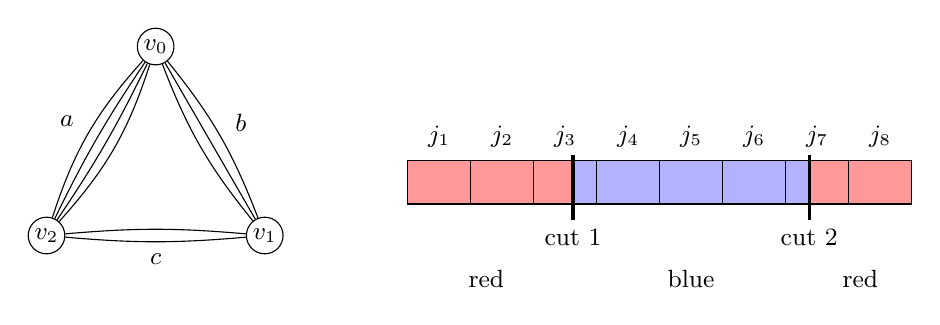
\begin{tikzpicture}[every node/.style={font=\small}]
  \begin{scope}
    \node[circle,draw,inner sep=1.2pt,fill=white] (v0) at (90:1.6) {$v_0$};
    \node[circle,draw,inner sep=1.2pt,fill=white] (v1) at (330:1.6) {$v_1$};
    \node[circle,draw,inner sep=1.2pt,fill=white] (v2) at (210:1.6) {$v_2$};
    \draw (v0) to[bend left=9] (v1); \draw (v0) -- (v1); \draw (v0) to[bend right=9] (v1);
    \draw (v1) to[bend left=5] (v2); \draw (v1) to[bend right=5] (v2);
    \draw (v2) to[bend left=12] (v0); \draw (v2) to[bend left=4] (v0);
    \draw (v2) to[bend right=4] (v0); \draw (v2) to[bend right=12] (v0);
    \node at (30:1.25) {$b$}; \node at (270:1.1) {$c$}; \node at (150:1.3) {$a$};
  \end{scope}
  \begin{scope}[xshift=3.2cm,yshift=-0.4cm]
    \fill[red!40] (0,0) rectangle (2.1,0.55);
    \fill[blue!30] (2.1,0) rectangle (5.1,0.55);
    \fill[red!40] (5.1,0) rectangle (6.4,0.55);
    \foreach \i in {0,...,8} \draw (0.8*\i,0) -- (0.8*\i,0.55);
    \draw (0,0) rectangle (6.4,0.55);
    \foreach \i in {1,...,8} \node at (0.8*\i-0.4,0.85) {$j_{\i}$};
    \draw[very thick] (2.1,-0.2) -- (2.1,0.62);
    \draw[very thick] (5.1,-0.2) -- (5.1,0.62);
    \node[below] at (2.1,-0.2) {cut 1};
    \node[below] at (5.1,-0.2) {cut 2};
    \node at (1.0,-0.95) {red};
    \node at (3.6,-0.95) {blue};
    \node at (5.75,-0.95) {red};
  \end{scope}
\end{tikzpicture}
\caption{Left: a cycle of three bundles $a,b,c$ of arbitrary sizes (here $4$, $3$ and $2$ items);
each function reads its two bundles through an arbitrary $1$-Lipschitz function. Right: a necklace
colouring of one bundle with $8$ items and $2$ cuts. Only the items containing a cut ($j_3$ and
$j_7$) receive a fractional colour, so a function reading two bundles sees at most $4$ fractional
items.}
\label{fig:cycle}
\end{figure}

\paragraph{The topological approach and its bottleneck.}
Lemma~9 of~\cite{HMMS25} places all items on $[0,1]$ and applies a consensus-halving theorem: with
at most $n$ cuts, all multilinear extensions are balanced. After rounding, a function errs by at
most the number of fractional items it reads, which may be all $n$ of them. For sparse families
we need \emph{local} control, so we give every bundle $e$ its own interval and allow it $k_e$
cuts. Colourings of $e$ with at most $k_e$ cuts form a sphere $S^{k_e}$ (the Hobby--Rice
parametrization~\cite{HR65,Pin76}), and the colour swap is the antipodal map. The composite
$\hG_v$ (the multilinear extension of $g_v$, evaluated on the necklace colourings) is a map on
the product of spheres $X=\prod_eS^{k_e}$. It depends only on the bundles $N(v)$ at $v$ and is
odd under flipping all of them simultaneously. If all $\hG_v$ vanish simultaneously, rounding
gives $|g_v|\le\sum_{e\in N(v)}k_e$.

The obvious symmetry is the \emph{diagonal} $\Z_2$, which flips every bundle. It is far too
weak. By itself it cannot force a common zero of more than $\min_ek_e$ odd functions (project $X$
to its smallest factor), whereas we have $n$ functions (Remark~\ref{rem:diagonal}).

\paragraph{The parity decomposition (Theorem~\ref{thm:C}).}
The function $\hG_v$ is \emph{not} odd in the individual bundles at $v$, but it can be split into
pieces that are. For $S\subseteq N(v)$ let
\[
  \hG_v^S(w)=2^{-d_v}\sum_{T\subseteq N(v)}(-1)^{|S\cap T|}\,\hG_v(\flip_Tw),
\]
where $\flip_T$ negates the coordinates of the bundles in $T$. Then $\hG_v=\sum_S\hG_v^S$, each
piece transforms by the character $U\mapsto(-1)^{|S\cap U|}$ of $(\Z_2)^{N(v)}$, and joint oddness
kills the pieces with $|S|$ even. For two bundles $a,b$ at $v$, this is simply
\[
  E_v(a,b)=\tfrac12\bigl(\hG_v(a,b)+\hG_v(a,-b)\bigr),\qquad
  O_v(a,b)=\tfrac12\bigl(\hG_v(a,b)-\hG_v(a,-b)\bigr),
\]
where $E_v$ is odd in $a$ and even in $b$, and $O_v$ is even in $a$ and odd in $b$. A common zero
of all pieces is a common zero of all $\hG_v$. For the triangle of Figure~\ref{fig:cycle}, with two
cuts per bundle, the six equations $E_0(a,b)$, $O_0(a,b)$, $E_1(b,c)$, $O_1(b,c)$, $E_2(c,a)$ and
$O_2(c,a)$ are odd in $a,b,b,c,c,a$, respectively, and even in the other variable. Each bundle
sphere $S^2$ thus carries exactly two equations that are odd in it, just as $S^k$ carries $k$ odd
equations in the Borsuk--Ulam theorem. The equations are coupled, so this is not Borsuk--Ulam on
each factor; the cohomological computation described next makes the heuristic precise. We have thus replaced the $\Z_2$-equivariant
problem by a $(\Z_2)^{\text{bundles}}$-equivariant one, at the cost of $2^{d_v-1}$ equations per
function. The Fadell--Husseini index~\cite{FH88} of $X$ with the factorwise action is the monomial
ideal $(t_e^{k_e+1})$. The Euler class of the target is a product of linear forms
$\sum_{e\in S}t_e$, one for each piece. This product is nonzero, and each of its monomials has
$t_e$-degree at most the number $k_e$ of pieces that are odd in $e$. Hence it lies outside the
monomial ideal, and an equivariant map must have a zero. For a cycle of bundles each bundle $e$ receives exactly two equations, one $E$ and
one $O$, from its two endpoints; the Euler class is $\prod_et_e^2$, two cuts per bundle suffice,
and every function reads at most $4$ fractional items.

\paragraph{Why one cut per bundle fails (Proposition~\ref{prop:torus}).}
With one cut per bundle the spheres become circles. On a cycle the topological statement would
read: continuous functions $f_i(\theta_i,\theta_{i+1})$ on tori, odd under the joint antipodal map,
have a common zero. We give explicit counterexamples of the form
$\sin(\theta_{i+1}-2\theta_i-c_i)$ and $\sin(2\theta_{i+1}-\theta_i-c_i)$, whose zero sets wind
inconsistently around the cycle. Hence two cuts per bundle are necessary for any argument
that uses only the oddness and locality of the $\hG_v$.

\paragraph{Combining (Theorem~\ref{thm:D}).}
We eliminate heavy functions one at a time. Let $v$ be heavy. Each lobe $L$ of $v$ interacts with
the rest of the instance only through the colouring of its ports. As seen from $L$, we replace $v$
by a new \emph{closing function} $c_L$ that reads exactly the ports through an \emph{arbitrary}
odd test function $\psi$. The closing function is light, because $L$ has at most $\Delta$ ports,
so the new instance has fewer heavy functions, and by induction it has a good colouring for every
$\psi$. Hence the set $T_L$ of port colourings that extend into $L$ meets every coarse zero set
$\{|\psi|\le C\}$, and by the loop-or-certificate dichotomy $T_L$ contains a loop. As in the tree
argument, the crossing lemma on the product of the lobes' loops then gives a colouring of $v$'s
items that is good for $v$ and extends into every lobe. When no heavy function is left,
Theorem~\ref{thm:C} applies.

\paragraph{Hub transfer and near-loops (Theorem~\ref{thm:F}).}
For $t=2$ we order the functions so that each has at most $d$ later neighbours and delete them
from last to first. When $h$ is deleted, an earlier neighbour $r$ loses the bundle $S=B_{hr}$. We
give $r$ the new constraint
\[
  \cG_r=\bigl\{\rho\in\cube T:\ \text{the slice }\{s\in\cube S:(s,\rho)\in Z_r\}\text{ contains a $1$-loop}\bigr\},
\]
where $T$ is the set of remaining items of $r$ and $Z_r$ its current constraint. If every
neighbour's new constraint is met, then $h$ sees a product of $1$-loops, one in each of its
bundles, and the crossing lemma gives $h$ a good value. The heart of the matter is that $\cG_r$ is
again a constraint of the same kind: if $Z_r$ contains the coarse zero set $\{|\psi|\le\ell\}$ of
an odd $2$-Lipschitz function, then $\cG_r$ contains such a set at level $\ell-1$. By the
loop-or-certificate dichotomy, this amounts to the following hub-transfer lemma: along every
antipodal $(\ell-1)$-path $\rho^0,\dots,\rho^L$ in $\cube T$, some slice
$\{s:|\psi(s,\rho^\tau)|\le\ell\}$ contains a $1$-loop. Call $B\subseteq\cube S$ \emph{thick} if every
antipodal $1$-path meets $B$. For each $\tau$ the cube $\cube S$ splits into
$P_\tau=\{\psi(\cdot,\rho^\tau)>\ell\}$, the slice, and $N_\tau=\{\psi(\cdot,\rho^\tau)<-\ell\}$, and
the Lipschitz condition gives $\dist(P_\tau,N_\tau)\ge3$ and $\dist(P_\tau,N_{\tau\pm1})\ge2$. Two
statements about a single cube finish the proof:
\begin{itemize}[leftmargin=*,itemsep=1pt]
\item (dichotomy) if $\dist(P,N)\ge3$ and the rest of the cube contains no $1$-loop, then $P$ or $N$
is thick;
\item (separation) two thick sets are at distance at most $1$.
\end{itemize}
If no slice contains a $1$-loop, then for each $\tau$ exactly one of $P_\tau,N_\tau$ is thick.
Oddness forces the thick side to differ at $\tau=0$ and $\tau=L$, and separation forbids a switch in
one step. We prove both statements on the $2$-skeleton of the cube coned off at the barycentres of
its squares. This complex is simply connected and carries a free involution, and its components
under a labelling correspond exactly to components in the cube, so nothing has to be rounded. Simple
connectivity makes the components of the label classes form a tree. The dichotomy then follows from
a separation lemma for graphs with a free involution. The separation follows from the Borsuk--Ulam
theorem, applied to a two-cut necklace sphere mapped into the complex and composed with the map to
the tree, embedded in $\R^2$. So each such deletion costs every earlier neighbour one level; since a
function has at most $d$ later neighbours, starting from level $d+1$ leaves level at least $1$ for
every function (Theorem~\ref{thm:Finst}). To do better we weaken the demand: instead of a $1$-loop,
the neighbour only guarantees a \emph{near-loop} of the shared bundle, a path with steps of length at
most $2$ that ends within distance $1$ of the antipode of its start. Dichotomy and separation hold for
near-loops as well (the dichotomy now with $\dist(P,N)\ge2$), so this demand costs the neighbour
nothing, and a deleted function at level $\ell$ can absorb the resulting deficiency from $\ell$
neighbours. Deleting in a degeneracy order with only such demands gives $\max(2,d)$, and charging each
edge to the endpoint it points to in an orientation of small in-degree gives $p+1$
(Theorem~\ref{thm:F}). For planar patterns, a canonical ordering splits the pattern into a
$2$-degenerate graph, whose edges are absorbed, and a forest, whose edges are charged to their
children; every function then pays at most one level, which gives $3$. Keeping track of the individual levels, the process
may stop at a forest whose level-$1$ vertices are pairwise non-adjacent: by an asymmetric version
of $\mathcal{K}_2=2$ (any two odd $2$-Lipschitz functions have a common point where one is at most $1$ and the
other at most $2$ in absolute value), such a forest is always solvable. This gives results for systems in which some functions are
held at level $1$ (Section~\ref{sec:leveled}).

\subsection{Related work}\label{sec:related}

\paragraph{Additive discrepancy.}
Beyond the results above~\cite{BF81,Spe85,Ban98,BJ25,BJ26}, constructive versions of partial
colouring~\cite{Ban10,LM15} underlie most modern algorithmic discrepancy. As discussed
in~\cite{HMMS25}, partial colouring breaks down for non-additive functions because the
discrepancies of partial colourings cannot be combined by the triangle inequality.

\paragraph{Non-additive discrepancy.}
Hollender, Manurangsi, Meka and Suksompong~\cite{HMMS25} (see~\cite{HMMS26} for the conference
version) and Dupr\'e la Tour and Fujii~\cite{DF25} proved $O(\sqrt{n\log n})$ bounds for $n$ arbitrary $1$-Lipschitz functions, with multicolour
extensions; the bound of~\cite{DF25} for $k$ colours is $O(\sqrt{n\log(nk)})$ when $k$ is a prime
power. Both works derive applications to consensus halving and envy-freeness up to $c$ goods, and
Dupr\'e la Tour and Fujii also derive an application to envy-freeness with subsidies. Hollender,
Manurangsi, Meka and Suksompong also proved the $O((mt)^{1/3}\log^{1/3}(mt))$ bound for $t$-sparse
families and raised Question~\ref{q:14}. Coverage-type special cases of sparse non-additive
discrepancy have also been studied: Avila, Rohwedder and Wennmann~\cite{ARW26} consider $t$-sparse
families of coverage functions and prove constructive bounds polynomial in $t$, the number of
colours, and $\log n$. Our results are of a different nature. We allow \emph{arbitrary}
$1$-Lipschitz functions and restrict the \emph{sparsity pattern}, and apart from Theorem~\ref{thm:dense} and Theorem~\ref{thm:F}(d) our bounds do not depend on
$n$ or $m$.

\paragraph{Consensus halving and necklaces.}
The existence of consensus halvings with $n$ cuts for $n$ non-additive valuations is due to
Simmons and Su~\cite{SS03}; the additive case goes back to the Hobby--Rice theorem~\cite{HR65}
(see~\cite{Pin76} for a Borsuk--Ulam proof) and to necklace splitting~\cite{Alo87}. The prime-$k$
generalization used in~\cite{HMMS25} is due to Filos-Ratsikas, Hollender, Sotiraki and
Zampetakis~\cite{FHSZ21}. Consensus halving for indivisible items was studied by Goldberg,
Hollender, Igarashi, Manurangsi and Suksompong~\cite{GHIMS20}. On the computational side,
approximate consensus halving is PPA-complete~\cite{FG18}, and its complexity has been mapped in
detail~\cite{FHSZ23}. Our necklace spheres are the configuration spaces of these proofs, used
bundle by bundle; products of necklace spheres with prescribed numbers of cuts in each direction
were used by de Longueville and \v{Z}ivaljevi\'c~\cite{dLZ08} to split multidimensional necklaces,
and the Borsuk--Ulam approach to necklace bisection goes back to Alon and West~\cite{AW86}.

\paragraph{Equivariant topology.}
The ideal-valued index is due to Fadell and Husseini~\cite{FH88}; see Matou\v{s}ek's
book~\cite{Mat03} for topological methods in combinatorics and the survey of Blagojevi\'c and
Ziegler~\cite{BZ17} for the ideal-valued index in combinatorial applications. Products of spheres
with $(\Z_2)^k$-actions, and the question whether an Euler class that is a product of linear forms
lies in the monomial ideal $(t_1^{d+1},\dots,t_k^{d+1})$, are central in the Gr\"unbaum--Hadwiger--Ramos
hyperplane mass-partition problem~\cite{Ram96,MVZ06,BFHZ18}; the character decomposition of a test
map used in our parity decomposition is a standard tool there~\cite{BFHZ18}. Antipodal paths in the
Hamming cube also appear in work on cube labellings with monochromatic antipodal paths, see Feder and
Subi~\cite{FS13}; our thick-set lemmas concern a different question (blocking all antipodal paths)
and are closer in spirit to Tucker's lemma. In our setting the obstruction can be
evaluated for every bundle hypergraph, because each monomial of the Euler class respects the
degree bounds termwise.

\paragraph{Organization.}
Section~\ref{sec:prelims} sets up the reformulation, bundles, the constants $\mathcal{K}_n$, multilinear
extensions and the consensus-halving lemma, and the notions of loops and separating sets.
Section~\ref{sec:small} proves Theorem~\ref{thm:Kn}, Section~\ref{sec:acyclic} proves
Theorem~\ref{thm:A} and its corollaries, and Section~\ref{sec:degree} proves Theorem~\ref{thm:C}.
Section~\ref{sec:torus} contains the torus counterexample, Section~\ref{sec:combine} proves
Theorem~\ref{thm:D}, Section~\ref{sec:degeneracy} proves Theorems~\ref{thm:F} and~\ref{thm:dense} and their
consequences, and Section~\ref{sec:open} lists open problems. Appendix~\ref{app:k3} documents the
computer-assisted part of Theorem~\ref{thm:Kn} and the ancillary files, and Appendix~\ref{sec:sat}
reports the SAT computations behind Conjecture~\ref{conj:two}. Readers interested mainly in the main
result can read Section~\ref{sec:prelims} and then Section~\ref{sec:degeneracy}, which is
self-contained apart from the constraint-system reformulation.

\section{Preliminaries}\label{sec:prelims}

\paragraph{Notation.}
$[r]=\{1,\dots,r\}$. For a finite set $U$ let $\cube{U}$ be the set of sign vectors indexed by
$U$, with Hamming distance $\dist$. For $A,A'\subseteq\cube{U}$ write $-A=\{-z:z\in A\}$,
$\dist(z,A)=\min_{a\in A}\dist(z,a)$ and $\dist(A,A')=\min_{a\in A}\dist(a,A')$, with
$\dist(\cdot,\emptyset)=\infty$. A set $A$ is \emph{symmetric} if $A=-A$. A function
$h\colon\cube{U}\to\R$ is \emph{odd} if $h(-z)=-h(z)$ and \emph{$L$-Lipschitz} if
$|h(z)-h(z')|\le L\dist(z,z')$. Since the Hamming distance is a path metric, it suffices to check
the Lipschitz condition for $\dist(z,z')=1$. For disjoint $U,W$ we write $(z,y)\in\cube{U\cup W}$
for the concatenation of $z\in\cube U$ and $y\in\cube W$.

\subsection{Imbalance functions and instances}

For $f\colon2^{[m]}\to\R$ define $g_f\colon\cube{[m]}\to\R$ by
$g_f(x)=f(\{j:x_j=1\})-f(\{j:x_j=-1\})$. The set $R(f)$ of items relevant to
$f$~\cite[Definition~13]{HMMS25} consists of the $j$ such that $f(S)\ne f(S\cup\{j\})$ for some
$S$. Analogously, coordinate $j$ is relevant to $g\colon\cube{[m]}\to\R$ if changing $x_j$ changes
$g(x)$ for some $x$.

\begin{lemma}\label{lem:imbalance}
\begin{enumerate}[label=(\alph*),itemsep=0pt]
\item If $f$ is $1$-Lipschitz, then $g_f$ is odd and $2$-Lipschitz, and it depends only on the
coordinates in $R(f)$.
\item If $g\colon\cube{[m]}\to\R$ is odd and $2$-Lipschitz, then
$f(S)=\tfrac12g(\mathbf 1_S-\mathbf 1_{[m]\setminus S})$ is $1$-Lipschitz, $g_f=g$, and $R(f)$ is
the set of coordinates relevant to $g$.
\item For every family $\cF=\{f_1,\dots,f_n\}$,
$\disc(\cF)=\min_{x\in\cube{[m]}}\max_i|g_{f_i}(x)|$.
\end{enumerate}
\end{lemma}

\begin{proof}
(a) Swapping the two colour classes negates $g_f$, so $g_f$ is odd. Changing $x_j$ moves item $j$
from one colour class to the other, so each of the two terms of $g_f$ changes by at most $1$, and
$g_f$ is $2$-Lipschitz. If $j\notin R(f)$, then $f(S)=f(S\cup\{j\})$ for all $S$, so moving $j$
does not change either term.
(b) If $S,S'$ differ in one element, then the vectors $\mathbf 1_S-\mathbf 1_{\bar S}$ and
$\mathbf 1_{S'}-\mathbf 1_{\bar S'}$ differ in one coordinate, so $|f(S)-f(S')|\le1$. Moreover
$g_f(x)=\frac12g(x)-\frac12g(-x)=g(x)$, and $f(S)\ne f(S\cup\{j\})$ holds exactly when $g$ changes
in coordinate $j$ at $\mathbf 1_S-\mathbf 1_{\bar S}$.
(c) This is the definition of discrepancy, with $\chi^{-1}(1)=\{j:x_j=1\}$.
\end{proof}

\begin{definition}[instances]\label{def:instance}
An \emph{instance} on the item set $[m]$ is a finite family $\cG=(g_v,U_v)_{v\in V}$, where each
$g_v\colon\cube{[m]}\to\R$ is odd and $2$-Lipschitz and depends only on the coordinates in its
\emph{support} $U_v\subseteq[m]$. We often regard $g_v$ as a function on $\cube{U_v}$. Its
\emph{discrepancy} is $\disc(\cG)=\min_{x}\max_{v}|g_v(x)|$. The instance is \emph{$t$-sparse} if
every item lies in at most $t$ supports.
\end{definition}

By Lemma~\ref{lem:imbalance}, a family $\cF$ of $1$-Lipschitz functions yields the instance
$\cG(\cF)=(g_{f},R(f))_{f\in\cF}$ with $\disc(\cG(\cF))=\disc(\cF)$, and $\cG(\cF)$ is $t$-sparse
if and only if $\cF$ is. Conversely, every instance with $U_v$ equal to the set of relevant
coordinates of $g_v$ arises from a family. Supports may be larger than the sets of relevant
coordinates. All our upper bounds are proved for instances under hypotheses on the supports, and
they apply to families through $\cG(\cF)$. An odd function with empty support is identically
zero.

\subsection{Bundles and the bundle hypergraph}

\begin{definition}[bundles]\label{def:bundles}
Let $\cG=(g_v,U_v)_{v\in V}$ be an instance. Items lying in no support are irrelevant, can be
coloured arbitrarily, and are ignored. For nonempty $S\subseteq V$ let
$B_S=\{j:\{v:j\in U_v\}=S\}$. The nonempty sets $B_S$ are the \emph{bundles}; they partition the
relevant items. A bundle with $|S|=1$ is \emph{private}. The \emph{bundle hypergraph} $H(\cG)$ has
vertex set $V$ and edge set $\{S:|S|\ge2,\ B_S\ne\emptyset\}$. The \emph{incidence graph}
$I(\cG)$ is the bipartite graph with classes $V$ and $\{S:B_S\ne\emptyset\}$, in which $v$ is
joined to $S$ if $v\in S$. We call $H(\cG)$ \emph{Berge-acyclic} if $I(\cG)$ is a forest. Private
bundles are leaves of $I(\cG)$, so it does not matter whether they are included.
\end{definition}

For a family $\cF$ we use the bundles of $\cG(\cF)$; then $B_S$ is the set of items whose set of
relevant functions is exactly $S$, as in Section~\ref{sec:results}. Berge-acyclicity forbids in
particular two hyperedges sharing two vertices, since these would form a $4$-cycle in $I(\cG)$.

\paragraph{The case $t=2$.}
For a $2$-sparse instance, the \emph{item multigraph} has vertex set $V$; every item lying in two
supports $U_u,U_v$ is an edge $uv$, and items lying in one support are private. Bundles with
$|S|=2$ are the parallel classes, $H(\cG)$ is the simple graph underlying the item multigraph, and
$H(\cG)$ is Berge-acyclic if and only if this simple graph is a forest. For a vertex $v$, the
number $d_v$ of hyperedges of $H(\cG)$ at $v$ is its number of distinct neighbours.

\subsection{The constants \texorpdfstring{$\mathcal{K}_n$}{K\_n}}

\begin{definition}\label{def:Kn}
For $n\ge1$ let $\mathcal{K}_n$ be the supremum of $\disc(\cG)$ over all $m\ge1$ and all instances $\cG$
with $n$ functions on the item set $[m]$. By Lemma~\ref{lem:imbalance}, this is also the supremum
of $\disc(\cF)$ over families of $n$ $1$-Lipschitz functions.
\end{definition}

Adding the zero function shows $\mathcal{K}_n\le \mathcal{K}_{n+1}$. By definition, every instance with at most $n$
functions has a colouring with $|g_v|\le \mathcal{K}_n$ for all $v$. The supremum is used only through this
property, so it does not matter whether it is attained.

\begin{lemma}\label{lem:Kbounds}
For every $n\ge1$, $\sqrt{n/2}\le \mathcal{K}_n<\sqrt{2n(1+\ln(2n))}$.
\end{lemma}

\begin{proof}
For $k=2$, Theorem~8 of~\cite{HMMS25} states that every $1$-Lipschitz family of $n$ functions has
$\disc(\cF,2)<\sqrt{2n(k-1)(1+\ln(nk))}=\sqrt{2n(1+\ln 2n)}$, and $\disc(\cF,2)$ is our
$\disc(\cF)$. For the lower bound, let $N=2^a$ and let $h_1,\dots,h_N$ be the rows of a Sylvester
Hadamard matrix ($\pm1$ entries, pairwise orthogonal rows). The functions $g_i(x)=\langle
h_i,x\rangle$ on $\cube{[N]}$ are odd and $2$-Lipschitz, and for every $x$ we have
$\max_i|g_i(x)|^2\ge\frac1N\sum_i\langle h_i,x\rangle^2=\frac1N\cdot N\|x\|_2^2=N$. Hence
$K_N\ge\sqrt N$. For general $n$ take $N=2^{\lfloor\log_2n\rfloor}>n/2$ and use monotonicity.
\end{proof}

The next lemma is needed only to state tightness for families in which sparsity is measured by
relevance.

\begin{lemma}\label{lem:allrelevant}
Let $g_1,\dots,g_n$ be odd $2$-Lipschitz functions on $\cube{[m]}$ and let $\varepsilon>0$. There
are odd $2$-Lipschitz $g_1',\dots,g_n'$ on $\cube{[m]}$ such that every coordinate is relevant to
every $g_i'$ and $\min_x\max_i|g_i'(x)|\ge\min_x\max_i|g_i(x)|-\varepsilon$.
\end{lemma}

\begin{proof}
Let $\ell(x)=\frac1m\sum_jx_j$ and $g_i'=(1-\delta)g_i+\delta\ell$ with $\delta\in(0,1)$. Each
$g_i'$ is odd and satisfies $|g_i'(x)-g_i'(x^{(j)})|\le2(1-\delta)+2\delta/m\le2$, where
$x^{(j)}$ is $x$ with coordinate $j$ flipped. Since $|g_i(x)|=\frac12|g_i(x)-g_i(-x)|\le m$, we
have $|g_i'-g_i|\le\delta(m+1)$. Fix $i$ and $j$. If $g_i$ does not depend on $x_j$, then
$g_i'(x)-g_i'(x^{(j)})=2\delta x_j/m\ne0$. Otherwise pick $x$ with $D=g_i(x)-g_i(x^{(j)})\ne0$; then
$g_i'(x)-g_i'(x^{(j)})=(1-\delta)D+2\delta x_j/m$, which vanishes for at most one value of
$\delta$. Choosing $\delta\le\varepsilon/(m+1)$ outside these finitely many values proves the
claim.
\end{proof}

\subsection{Multilinear extensions and the consensus-halving lemma}

For $g\colon\cube{[m]}\to\R$ and $x\in[-1,1]^m$ let $\xi^x\in\cube{[m]}$ be the random vector with
independent coordinates and $\Pr[\xi^x_j=1]=\frac{1+x_j}2$, so that $\E\xi^x_j=x_j$. The
\emph{multilinear extension} of $g$ is $G(x)=\E[g(\xi^x)]$. A coordinate $j$ of $x$ is
\emph{fractional} if $x_j\in(-1,1)$.

\begin{lemma}\label{lem:multilinear}
Let $g\colon\cube{[m]}\to\R$ be odd and $2$-Lipschitz, depending only on the coordinates in $U$,
and let $G$ be its multilinear extension. Then:
\begin{enumerate}[label=(\alph*),itemsep=0pt]
\item $G=g$ on $\cube{[m]}$, $G$ depends only on the coordinates in $U$, and $G$ is continuous;
\item $G$ is odd: $G(-x)=-G(x)$;
\item $G$ is $1$-Lipschitz with respect to $\ell_1$: $|G(x)-G(x')|\le\|x-x'\|_1$;
\item if $G(x)=0$ and $x'\in\cube{[m]}$ is obtained from $x$ by replacing every fractional
coordinate by a nearest sign, then $|g(x')|$ is at most the number of fractional coordinates of
$x$ in $U$.
\end{enumerate}
\end{lemma}

\begin{proof}
(a) If $x\in\cube{[m]}$ then $\xi^x=x$. The distribution of $\xi^x|_U$ depends only on $x|_U$, and
$G$ is a polynomial in $x$. (b) The vector $-\xi^x$ has the distribution of $\xi^{-x}$, so
$G(-x)=\E g(-\xi^x)=-G(x)$. (c) Let $h(S)=\frac12g(\mathbf 1_S-\mathbf 1_{[m]\setminus S})$, which
is $1$-Lipschitz on $\{0,1\}^m$, and let $\bar h(p)=\E_{S\sim D_p}h(S)$ be its multilinear
extension on $[0,1]^m$ in the sense of~\cite{HMMS25}, where $D_p$ includes each $j$ independently
with probability $p_j$. By~\cite[Lemma~16]{HMMS25}, $\bar h$ is $1$-Lipschitz with respect to
$\ell_1$. Since $\xi^x=\mathbf 1_S-\mathbf 1_{\bar S}$ with $S\sim D_{(\mathbf 1+x)/2}$, we have
$G(x)=2\bar h(\frac{\mathbf 1+x}2)$, and therefore
$|G(x)-G(x')|\le2\|\frac{x-x'}2\|_1=\|x-x'\|_1$. (d) Rounding changes each fractional coordinate by
at most $1$ and leaves the others unchanged, so by (a) and (c),
$|g(x')|=|G(x')-G(x)|\le\sum_{j\in U}|x_j-x'_j|$, which is at most the number of fractional
coordinates in $U$.
\end{proof}

We now recall the consensus-halving lemma of~\cite{HMMS25} for two colours. Theorem~5
of~\cite{HMMS25}, due to Simmons and Su~\cite{SS03} for $k=2$ and to Filos-Ratsikas, Hollender,
Sotiraki and Zampetakis~\cite{FHSZ21} for prime $k$, reads as follows for $k=2$: \emph{for any
utility functions $u_1,\dots,u_n$ on the Borel subsets of $[0,1]$ satisfying the continuity
condition of~\cite[Assumption~4]{HMMS25}, it is possible to partition $[0,1]$ into two pieces
$A_1,A_2$ using at most $n$ cuts so that $u_i(A_1)=u_i(A_2)$ for all $i$.} Placing item $j$ on the
interval $[\frac{j-1}m,\frac jm]$ yields Lemma~9 of~\cite{HMMS25}, which for $k=2$ reads:
\emph{for any $1$-Lipschitz $f_1,\dots,f_n\colon\{0,1\}^m\to\R$ there is a fractional
$2$-colouring $\chi$ with at most $n$ fractional elements such that
$\bar f_i(\chi_1)=\bar f_i(\chi_2)$ for all $i$}. Here $\chi_1\in[0,1]^m$, $\chi_2=\mathbf
1-\chi_1$, and $\bar f$ is the multilinear extension. In our language:

\begin{corollary}\label{cor:lemma9}
For odd $2$-Lipschitz $g_1,\dots,g_n$ on $\cube{[m]}$ there is $x\in[-1,1]^m$ with at most $n$
fractional coordinates such that $G_i(x)=0$ for all $i$.
\end{corollary}

\begin{proof}
Apply~\cite[Lemma~9]{HMMS25} to the $1$-Lipschitz functions
$f_i(S)=\frac12g_i(\mathbf 1_S-\mathbf 1_{\bar S})$ (Lemma~\ref{lem:imbalance}(b)), obtaining
$p=\chi_1$. If $S\sim D_p$, then $[m]\setminus S\sim D_{\mathbf 1-p}$, so
$0=\bar f_i(p)-\bar f_i(\mathbf 1-p)=\E[f_i(S)-f_i([m]\setminus S)]=\E[g_i(\mathbf 1_S-\mathbf
1_{\bar S})]=G_i(2p-\mathbf 1)$. Take $x=2p-\mathbf 1$; its fractional coordinates are those of
$p$.
\end{proof}

Equivalently, let $r\le n$ be the number of fractional coordinates of $x$. The law of $\xi^x$ is a
product distribution with full support on the $r$-dimensional subcube
$\{z\in\cube{[m]}:z_j=x_j\text{ for all integral }j\}$, and every $g_i$ has mean $0$ under it.

\subsection{Loops and separating sets}

\begin{definition}\label{def:loops}
Let $U\ne\emptyset$ be finite and let $s,r\ge0$ be reals.
\begin{itemize}[itemsep=0pt]
\item An \emph{$s$-path} in $A\subseteq\cube U$ is a sequence $z_0,\dots,z_L\in A$ with
$\dist(z_{i-1},z_i)\le s$ for all $i$. It is \emph{antipodal} if $z_L=-z_0$. The set $A$
\emph{contains an $s$-loop} if it contains an antipodal $s$-path.
\item A set $A\subseteq\cube U$ is \emph{$r$-separating} if $\cube U\setminus A=A^+\sqcup A^-$
with $A^-=-A^+$ and $\dist(A^+,A^-)>r$. (The set $A=\cube U$ is $r$-separating with
$A^\pm=\emptyset$.) Separating sets are symmetric.
\end{itemize}
\end{definition}

\begin{lemma}[crossing]\label{lem:crossing}
If $g$ is odd and $2$-Lipschitz and $z_0,\dots,z_L$ is an antipodal $s$-path, then
$|g(z_i)|\le s$ for some $i$.
\end{lemma}

\begin{proof}
Consecutive values differ by at most $2s$, and $g(z_L)=-g(z_0)$. If $g(z_0)=0$ we are done.
Otherwise the values change sign, so there are consecutive values $a,b$ with $a>0\ge b$ or $a<0\le
b$. Then $|a|+|b|=|a-b|\le2s$, so $\min(|a|,|b|)\le s$.
\end{proof}

\begin{lemma}[certificates]\label{lem:certificate}
\begin{enumerate}[label=(\alph*),itemsep=0pt]
\item If $A\subseteq\cube U$ is $r$-separating, then
$\varphi_A=\dist(\cdot,A^-)-\dist(\cdot,A^+)$ (and $\varphi_A\equiv0$ if $A=\cube U$) is odd and
$2$-Lipschitz, and $\{z:|\varphi_A(z)|\le r\}\subseteq A$.
\item If $A\subseteq\cube U$ is nonempty and symmetric and contains no $s$-loop, then there is
an odd $2$-Lipschitz $\psi$ on $\cube U$ with $|\psi|>s$ on $A$.
\end{enumerate}
\end{lemma}

\begin{proof}
(a) Distance functions are $1$-Lipschitz, so $\varphi_A$ is $2$-Lipschitz. Since $A^-=-A^+$, we
have $\dist(-z,A^-)=\dist(z,A^+)$, so $\varphi_A$ is odd. On $A^+$, $\varphi_A=\dist(\cdot,A^-)>r$,
and on $A^-$, $\varphi_A<-r$.
(b) Consider the graph on $A$ joining points at distance at most $s$. If a connected component
$C$ contained both $z$ and $-z$, a path in $C$ from $z$ to $-z$ would be an $s$-loop. Since $z\mapsto
-z$ is an isometry preserving $A$, it maps components to components, so the components come in
pairs $\{C,-C\}$ with $C\ne-C$. Let $A^+$ contain one component from each pair, and let
$A^-=-A^+$. Then $A=A^+\sqcup A^-$ and $\dist(A^+,A^-)>s$. The function
$\psi=\dist(\cdot,A^-)-\dist(\cdot,A^+)$ is odd and $2$-Lipschitz as in (a), and $|\psi|>s$ on
$A$.
\end{proof}

\begin{lemma}[loops]\label{lem:loop}
Let $q\ge0$ and let $\varphi_1,\dots,\varphi_q$ be odd $2$-Lipschitz functions on $\cube U$. Then
$J=\{z:|\varphi_j(z)|\le \mathcal{K}_{q+1}\ \text{for all } j\}$ contains a $\mathcal{K}_{q+1}$-loop.
\end{lemma}

\begin{proof}
$J$ is symmetric because the $\varphi_j$ are odd. It is nonempty: for $q=0$, $J=\cube U$; for
$q\ge1$, the definition of $\mathcal{K}_q\le \mathcal{K}_{q+1}$ gives a point with $\max_j|\varphi_j|\le \mathcal{K}_q$.
Suppose $J$ contains no $\mathcal{K}_{q+1}$-loop. By Lemma~\ref{lem:certificate}(b) there is an odd
$2$-Lipschitz $\psi$ with $|\psi|>\mathcal{K}_{q+1}$ on $J$. The instance $(\varphi_1,\dots,\varphi_q,\psi)$
on the item set $U$ has $q+1$ functions, so some $z$ satisfies $|\varphi_j(z)|\le \mathcal{K}_{q+1}$ for all
$j$ and $|\psi(z)|\le \mathcal{K}_{q+1}$. Then $z\in J$ and $|\psi(z)|\le \mathcal{K}_{q+1}$, a contradiction.
\end{proof}

\section{Small values: \texorpdfstring{$\mathcal{K}_1=1$}{K1=1} and \texorpdfstring{$\mathcal{K}_2=\mathcal{K}_3=2$}{K2=K3=2}}\label{sec:small}

\begin{restate}{Theorem~\ref{thm:Kn}, first part}
$\mathcal{K}_1=1$ and $\mathcal{K}_2=\mathcal{K}_3=2$. (The value $\mathcal{K}_4=3$ is proved in
Section~\ref{sec:k4}.)
\end{restate}

\subsection{Lower bounds and \texorpdfstring{$\mathcal{K}_1$}{K1}}

\begin{proof}[Proof of $\mathcal{K}_1=1$ and of the lower bounds]
Let $g$ be odd and $2$-Lipschitz on $\cube{[m]}$ and let $x\in\cube{[m]}$. Flipping the coordinates
of $x$ one at a time gives an antipodal $1$-path from $x$ to $-x$, and Lemma~\ref{lem:crossing}
yields a point with $|g|\le1$, so $\mathcal{K}_1\le1$. The function $g=x_1$ is odd and $2$-Lipschitz with
$|g|\equiv1$, so $\mathcal{K}_1\ge1$. The functions $g_1=x_1+x_2$ and $g_2=x_1-x_2$ are odd and $2$-Lipschitz,
and for every $x$ one of them equals $\pm2$; hence $\mathcal{K}_3\ge \mathcal{K}_2\ge2$.
\end{proof}

\subsection{Upper bounds via few fractional coordinates}

Let $g_1,\dots,g_n$ be odd and $2$-Lipschitz on $\cube{[m]}$ with $n\le3$. By
Corollary~\ref{cor:lemma9} there is $x$ with $r\le n$ fractional coordinates and $G_i(x)=0$ for
all $i$. Let $Q$ be the $r$-dimensional subcube of points agreeing with $x$ on its integral
coordinates. Write $w_z=\Pr[\xi^x=z]$ for $z\in Q$; these are product weights, all positive. Then
\begin{equation}\label{eq:meanzero}
  \textstyle\sum_{z\in Q}w_z\,g_i(z)=0\qquad\text{for } i=1,\dots,n,
\end{equation}
and each $g_i$ changes by at most $2$ along every edge of $Q$. Call $z\in Q$ \emph{bad for $i$} if
$|g_i(z)|>2$, and \emph{good} if it is bad for no $i$. A good corner $z$ is a colouring with
$\max_i|g_i(z)|\le2$, so it suffices to show that a good corner exists.

\begin{lemma}\label{lem:onefrac}
Let $a,b$ be reals with $|a-b|\le2$, and suppose $\alpha a+\beta b=0$ for some $\alpha,\beta>0$.
Then $|a|,|b|\le2$.
\end{lemma}

\begin{proof}
Either $a=b=0$, or $a$ and $b$ have opposite signs, say $a>0>b$. In the latter case
$a<a-b\le2$ and $-b<a-b\le2$.
\end{proof}

\begin{lemma}[corner lemma]\label{lem:corner}
Let $v$ be a real function on the four corners of a square (a $4$-cycle) such that adjacent
values differ by at most $2$, and let $w$ be positive weights with $\sum_xw_xv_x=0$. Then at most
one corner $x$ has $|v_x|>2$.
\end{lemma}

\begin{proof}
If $v_x>2$, then every neighbour $y$ of $x$ has $v_y\ge v_x-2>0$; similarly for $v_x<-2$. Two
corners with $v_x>2$ and $v_{x'}<-2$ would satisfy $|v_x-v_{x'}|>4$, while any two corners of a
square are at distance at most $2$, so their values differ by at most $4$. Hence any two bad
corners have the same sign, say positive. If they are adjacent, each of the other two corners is
adjacent to one of them; if they are opposite, each of the other two corners is adjacent to both.
In either case all four values are positive, contradicting $\sum_xw_xv_x=0$.
\end{proof}

\begin{proof}[Proof of $\mathcal{K}_2\le2$, and of $\mathcal{K}_3\le2$ when $r\le2$]
If $r=0$, then $Q=\{x\}$ and $g_i(x)=G_i(x)=0$. If $r=1$, then $Q=\{z,z'\}$ is an edge, and by
\eqref{eq:meanzero} and Lemma~\ref{lem:onefrac} both corners are good. If $r=2$, then $Q$ is a
square, and by \eqref{eq:meanzero} and Lemma~\ref{lem:corner} every function has at most one bad
corner; since $n\le3<4$, some corner is good. For $n=2$ we always have $r\le2$, which proves
$\mathcal{K}_2\le2$.
\end{proof}

\subsection{Three fractional coordinates: the computer-assisted step}\label{sec:k3}

It remains to treat $n=3$ and $r=3$. Identify $Q$ with $\{0,1\}^3$ through the three fractional
coordinates, where a coordinate equal to $+1$ corresponds to $1$. The weights are
$w_y(p)=\prod_{k=1}^3p_k^{y_k}(1-p_k)^{1-y_k}$ with $p\in(0,1)^3$. Write $v^i_y=g_i(y)$.
Suppose, for a contradiction, that no corner is good. Assign every corner to one function for
which it is bad. This gives a partition $\{0,1\}^3=T_1\sqcup T_2\sqcup T_3$, with some parts
possibly empty, such that every $y\in T_i$ is bad for $i$.

\begin{lemma}\label{lem:parts}
Each nonempty $T_i$ is either \emph{one-signed} ($v^i>2$ on $T_i$, or $v^i<-2$ on $T_i$) or a
\emph{mixed antipodal pair} $T_i=\{y,\bar y\}$ with $\bar y=\mathbf 1-y$ and $v^i_y>2>-2>v^i_{\bar
y}$.
\end{lemma}

\begin{proof}
If $v^i_y>2$ and $v^i_{y'}<-2$, then $2\dist(y,y')\ge|v^i_y-v^i_{y'}|>4$, so $\dist(y,y')=3$, that
is, $y'=\bar y$. Hence if $T_i$ contains points of both signs, every positive point is antipodal to
every negative point. A point has only one antipode, so $T_i$ consists of exactly one positive
point and its antipode.
\end{proof}

\begin{lemma}\label{lem:necessary}
Let $X$ be distributed according to the weights $w(p)$.
\begin{enumerate}[label=(\alph*),itemsep=0pt]
\item If $T=T_i$ is one-signed, then $\E[\dist(X,T)]>1$.
\item If $T_i=\{y,\bar y\}$ is a mixed antipodal pair with $v^i_y>2$, then
$1<\E[\dist(X,y)]<2$.
\end{enumerate}
\end{lemma}

\begin{proof}
(a) Replacing $v^i$ by $-v^i$ if necessary (this preserves \eqref{eq:meanzero}), assume $v^i>2$ on
$T$. For every corner $z$ and every $y\in T$ we have $v^i_z\ge v^i_y-2\dist(z,y)>2-2\dist(z,y)$, so
$v^i_z>2-2\dist(z,T)$. Multiplying by $w_z>0$, summing, and using \eqref{eq:meanzero} gives
$0>2-2\E[\dist(X,T)]$.
(b) As in (a), $v^i_z>2-2\dist(z,y)$. Also $v^i_z\le v^i_{\bar y}+2\dist(z,\bar
y)<-2+2(3-\dist(z,y))=4-2\dist(z,y)$. Summing with the weights gives $0>2-2\E\dist(X,y)$ and
$0<4-2\E\dist(X,y)$.
\end{proof}

Since $\dist(X,\bar y)=3-\dist(X,y)$, condition (b) is symmetric in $y$ and $\bar y$. A
\emph{configuration} consists of a labelling $\lambda\colon\{0,1\}^3\to\{1,2,3\}$ (the parts
$T_i=\lambda^{-1}(i)$) and, for every nonempty part that is an antipodal pair, a choice of type
(one-signed or mixed). There are $3^8=6561$ labellings and $7365$ configurations. Each condition in
Lemma~\ref{lem:necessary} has the form $\sum_y\rho_y w_y(p)>0$ for an integer vector $\rho$:
$\rho_y=\dist(y,T)-1$ in case (a), and $\rho_y=\dist(y,y_0)-1$ and $\rho_y=2-\dist(y,y_0)$ in case
(b), where $y_0$ is the corner of the pair with $v^i_{y_0}>2$. The left-hand side is a multilinear
polynomial in $p$.

\begin{lemma}[computer-assisted]\label{lem:computer}
For each of the $7365$ configurations, the conditions of Lemma~\ref{lem:necessary} have no
common solution $p\in[0,1]^3$.
\end{lemma}

\begin{proof}[Verification]
A multilinear polynomial on a box $\prod_k[a_k,b_k]$ is the multilinear interpolation of its
values at the $8$ vertices. Its value at any point of the box is therefore a convex combination of
the vertex values, and if it is $\le0$ at all vertices, it is $\le0$ on the box. For each
configuration, a branch-and-bound procedure starts with the box $[0,1]^3$. A box is
\emph{cleared} if one of the configuration's polynomials is $\le0$ at all $8$ vertices, so that
the corresponding strict condition fails on the whole box. Otherwise the box is bisected along its
longest side. All evaluations use exact rational arithmetic. The procedure clears every
configuration, with $20{,}613$ boxes in total and subdivision depth at most $6$
(Appendix~\ref{app:k3}). Every point $p\in[0,1]^3$ lies in a cleared box, so some condition fails
at $p$.
\end{proof}

\begin{proof}[Proof of $\mathcal{K}_3\le2$ when $r=3$]
If no corner were good, Lemmas~\ref{lem:parts} and~\ref{lem:necessary} would give a configuration
whose conditions all hold at the actual $p\in(0,1)^3$, contradicting Lemma~\ref{lem:computer}.
Hence a good corner exists. Together with the case $r\le2$, this proves $\mathcal{K}_3\le2$ and completes
the proof of Theorem~\ref{thm:Kn}.
\end{proof}

\begin{remark}\label{rem:K4}
The product structure of the weights is essential for Lemma~\ref{lem:computer}. If $w$ is an
arbitrary probability vector on $\{0,1\}^3$, the conditions of Lemma~\ref{lem:necessary} can be
satisfied. For instance, take $T_1=\{y:|y|\le1\}$, $T_2=\{y:|y|=2\}$, $T_3=\{\mathbf 1\}$, all
one-signed, and put weight $0.4$ on $\mathbf 0$ and $0.6$ on $\mathbf 1$. The three expectations
are then $1.2,1.4,1.2>1$, and they remain $>1$ after a small perturbation making all weights
positive. For four functions the corner method cannot prove $\mathcal{K}_4\le2$, because $\mathcal{K}_4\ge3$: the four additive
functions $g_p(x)=\langle p,x\rangle$ on three items, $p\in\{(1,1,1),(1,-1,-1),(-1,1,-1),(-1,-1,1)\}$,
satisfy $\max_p|g_p(x)|=3$ for every $x\in\cube{3}$, because the eight vectors $\pm p$ are exactly the
points of $\cube3$. So $\mathcal{K}_4\ge3>\mathcal{K}_3$ (Proposition~\ref{prop:t3} gives a $3$-sparse witness). The
matching upper bound is proved in Section~\ref{sec:k4}.
\end{remark}

\subsection{Four functions, and sparse families of five functions}\label{sec:k4}

We extend the corner method to threshold $c$ and to functions that read only some of the
fractional coordinates. Let $J$ be a finite set, let $w$ be a product distribution on $\cube J$
with full support, and let $X\sim w$.

\begin{lemma}\label{lem:necessaryc}
Let $c>0$, $J'\subseteq J$, and let $h\colon\cube{J'}\to\R$ be $2$-Lipschitz with
$\E\,h(X|_{J'})=0$. Let $U^+=\{u:h(u)>c\}$ and $U^-=\{u:h(u)<-c\}$. If $U^+\ne\emptyset$ then
$\E\dist(X|_{J'},U^+)>c/2$, if $U^-\ne\emptyset$ then $\E\dist(X|_{J'},U^-)>c/2$, and if both are
nonempty then $\dist(U^+,U^-)>c$. These conditions remain true when $U^+$ and $U^-$ are replaced by
nonempty subsets.
\end{lemma}

\begin{proof}
For every $u\in U^+$ and every $z$, $h(z)\ge h(u)-2\dist(z,u)>c-2\dist(z,u)$, so
$h(z)>c-2\dist(z,U^+)$; taking expectations gives $0>c-2\E\dist(X|_{J'},U^+)$. The case of $U^-$ is
symmetric, and $h(u)-h(u')>2c$ for $u\in U^+$, $u'\in U^-$ gives $2\dist(u,u')>2c$. Shrinking the
sets can only increase the distances.
\end{proof}

\begin{theorem}[computer-assisted]\label{thm:H}
\begin{enumerate}[label=(\alph*),itemsep=0pt]
\item $\mathcal{K}_4\le3$.
\item Every $2$-sparse instance with at most five functions has discrepancy at most $2$.
\end{enumerate}
\end{theorem}

\begin{proof}[Reduction and verification]
Let $c=3$, $n=4$ in (a) and $c=2$, $n\le5$ in (b). By Corollary~\ref{cor:lemma9} there is a point
$x$ with a set $J$ of $j\le n$ fractional coordinates at which all multilinear extensions vanish.
Fix the integral coordinates and let $w$ be the product distribution on $\cube J$ with means $x_e$;
it has full support. The restriction $h_i$ of $g_i$ depends only on the set $J_i\subseteq J$ of
fractional items in its support, is $2$-Lipschitz, and has $\E\,h_i=0$. In (a), $J_i=J$; in (b),
every $e\in J$ lies in $J_i$ for at most two indices $i$. If no corner of $\cube J$ satisfies
$|h_i|\le c$ for all $i$, then the sets $U_i^\pm$ of Lemma~\ref{lem:necessaryc} cover $\cube J$, in
the sense that every corner $z$ has some $i$ with $z|_{J_i}\in U_i^+\cup U_i^-$, and they satisfy
the conditions of the lemma at the actual means. Negating a coordinate of $\cube J$ in all functions
replaces its mean $x_e$ by $-x_e$ and preserves all hypotheses, so we may assume
$p_e=\Pr[X_e=1]\le\frac12$ for all $e$. Each condition $\E\dist(X|_{J_i},U)>c/2$ is a multilinear
function of $p$, so if it fails at all vertices of a box it fails on the whole box.

The verification runs a branch-and-bound over dyadic boxes in $[0,\frac12]^j$ for every $j\le n$
and, in (b), every sparsity pattern (an assignment of each of the $j$ items to a set of one or two of
the five functions, up to relabelling the functions; $1,2,7,22,69,198$ patterns for
$j=0,\dots,5$). In each box it lists, for each function, the pairs $(U^+,U^-)$ that satisfy the
conditions at some vertex, and a depth-first search confirms that no choice of one such pair per
function covers $\cube J$; otherwise the box is bisected. All comparisons are exact. For (a) all
boxes are cleared with $13$ boxes for $j=4$; for (b) all $299$ patterns are cleared with $1213$ boxes
in total and subdivision depth at most $3$. Two independently written programs, and two further
re-verifications of all leaf boxes, agree (Appendix~\ref{app:k3}). As a sanity check, the same
search does not clear $(n,c)=(4,2)$, $(2,1.9)$, $(3,1.9)$, $(4,2.9)$, or the $3$-sparse pattern of
Proposition~\ref{prop:t3} at $c=2$. In each of these cases it exhibits an interior point $p$ at which
the conditions admit a cover. Hence in (a) and (b) some corner is good, which gives the stated
bounds.
\end{proof}

\begin{proof}[Proof of $\mathcal{K}_4=3$]
$\mathcal{K}_4\ge3$ by Remark~\ref{rem:K4} and $\mathcal{K}_4\le3$ by Theorem~\ref{thm:H}(a).
\end{proof}

By Lemma~\ref{lem:good}, Theorem~\ref{thm:H}(b) says that every simple graph on at most five vertices
is $2$-good, so by Corollary~\ref{cor:onesum} every $2$-sparse instance whose blocks have at most five
vertices has discrepancy at most $2$.

\subsection{Real thresholds: six functions, and \texorpdfstring{$\mathcal{K}_5$}{K5}, \texorpdfstring{$\mathcal{K}_6$}{K6}}\label{sec:realc}

The corner method becomes much stronger if it is run at a threshold slightly below the next
integer. This rests on the following per-function version of Lemma~\ref{lem:cover} (Appendix~\ref{sec:sat}),
with the same proof.

\begin{lemma}\label{lem:integrality}
Let $(U_v)_{v\in V}$ be supports and $D_v\ge1$ integers. If some instance with these supports has, for
every $x$, some $v$ with $|g_v(x)|>D_v-1$, then some instance with the same supports has, for every
$x$, some $v$ with $|g_v(x)|\ge D_v$. Consequently, if for a class of support structures every instance
has a colouring with $|g_v|\le c_v$ for all $v$, where $c_v\in[D_v-1,D_v)$, then every such instance
has a colouring with $|g_v|\le D_v-1$ for all $v$.
\end{lemma}

\begin{proof}
Let $P_v=\{z\in\cube{U_v}:g_v(z)>D_v-1\}$. For $z,z'\in P_v$ we have
$2\dist(z,-z')\ge g_v(z)+g_v(z')>2D_v-2$, so $\dist(z,-z')\ge D_v$. The function
$g'_v=\dist(\cdot,-P_v)-\dist(\cdot,P_v)$ ($g'_v\equiv0$ if $P_v=\emptyset$) is odd and $2$-Lipschitz,
depends only on $U_v$, and satisfies $|g'_v|\ge D_v$ on $P_v\cup(-P_v)$, which contains $x|_{U_v}$ for
some $v$, for every $x$. The second statement follows by applying the first to an instance violating
the thresholds $D_v-1$.
\end{proof}

Thus Theorem~\ref{thm:H}(b) only needs a threshold $c<3$, and $\mathcal{K}_n\le D-1$ follows from
$\mathcal{K}_n<D$. We run the reduction in the proof of Theorem~\ref{thm:H} with real thresholds
$c_v$: by Corollary~\ref{cor:lemma9} and Lemma~\ref{lem:necessaryc}, if some instance with the given
supports has no colouring with $|g_v|\le c_v$ for all $v$, then for some $j\le n$, some pattern of
$j$ fractional items and some $p\in(0,\frac12]^j$ there are sets $U_v^\pm$ with
$\dist(U_v^+,U_v^-)\ge\lfloor c_v\rfloor+1$ and $\E\dist(X|_{J_v},U_v^\pm)>c_v/2$ for the nonempty parts,
which cover $\cube j$. (At a fixed $p$ these conditions are also sufficient for mean-zero $2$-Lipschitz
residuals that are bad at every corner: if both parts are nonempty, a convex combination of
$c_v+\varepsilon-2\dist(\cdot,U_v^+)$ and $-c_v-\varepsilon+2\dist(\cdot,U_v^-)$ has mean $0$, and if only
$U_v^+$ is nonempty, subtract its mean from $c_v+\varepsilon-2\dist(\cdot,U_v^+)$. So the box relaxation is
the only loss of the method relative to the residuals.) The branch-and-bound is that of
Theorem~\ref{thm:H}; with several thresholds, two functions are exchanged by the symmetry breaking only
if they read the same items and have the same threshold.

\begin{theorem}[computer-assisted]\label{thm:six}
\begin{enumerate}[label=(\alph*),itemsep=0pt]
\item Every $2$-sparse instance with at most six functions has discrepancy at most $2$.
\item $\mathcal{K}_5=3$ and $\mathcal{K}_6=4$; moreover $\mathcal{K}_8\ge5$.
\end{enumerate}
\end{theorem}

\begin{proof}
(a) By Lemma~\ref{lem:integrality} it suffices to clear the threshold $c=2.99$. Up to relabelling the
functions there are $2,7,23,76,245,782$ sparsity patterns of $j=1,\dots,6$ items on six functions
(these numbers agree with Burnside's lemma). All of them are cleared, with fewer than $1700$ boxes in
total, by two independently written programs, each run on its own enumeration of the patterns
(Appendix~\ref{app:k3}).

(b) Lower bounds: $\mathcal{K}_5\ge\mathcal{K}_4=3$. The six additive functions
$\langle a_i,x\rangle$ on six items with $a_1=-\mathbf 1$, $a_2=(1,1,-1,-1,-1,-1)$,
$a_3=(1,-1,1,-1,-1,-1)$, $a_4=(-1,1,1,1,-1,-1)$, $a_5=(-1,1,1,-1,1,-1)$, $a_6=(1,-1,-1,1,1,-1)$ satisfy
$\max_i|\langle a_i,x\rangle|\ge4$ for all $x\in\cube6$: $|\langle a_i,x\rangle|=6-2\dist(x,\pm a_i)\ge4$
if and only if $\dist(x,\pm a_i)\le1$, and the twelve balls of radius $1$ around the $\pm a_i$ cover
$\cube6$. Similarly, one word from each complementary pair of the Hamming $[7,4]$ code (which contains
$\mathbf 1$) gives eight additive functions on seven items with $\max_i|\langle a_i,x\rangle|\ge5$, since
the code is perfect of radius $1$; so $\mathcal{K}_8\ge5$. Upper bounds: by Lemma~\ref{lem:integrality}
it suffices to clear $c=3.99$ for five functions and $c=4.99$ for six functions, all reading all $j\le n$
fractional items; the branch-and-bound needs $1,1,1,3,29$ and $1,1,1,1,3,15$ boxes, respectively, for
$j=1,2,\dots$ (two programs, identical counts). As sanity checks, the same program fails for four
functions at $c=2.99$ and for six functions at $c=3.99$, in accordance with $\mathcal{K}_4=3$ and
$\mathcal{K}_6\ge4$.
\end{proof}

In particular $K_6$, $K_{3,3}$ and the octahedron, with arbitrary bundle sizes and private items, carry
only families of discrepancy at most $2$, and by Corollary~\ref{cor:onesum} so does every pattern whose
blocks have at most six vertices. The values $\mathcal{K}_1,\dots,\mathcal{K}_6$ are $1,2,2,3,3,4$.

\section{Acyclic sparsity patterns}\label{sec:acyclic}

\begin{theorem}\label{thm:Ainst}
Let $\cG=(g_v,U_v)_{v\in V}$ be a $t$-sparse instance whose bundle hypergraph is Berge-acyclic.
Then $\disc(\cG)\le \mathcal{K}_t$.
\end{theorem}

\begin{proof}
Let $c=\mathcal{K}_t$. Functions with empty support are identically zero and are isolated in $I(\cG)$, so
we drop them. Different trees of the forest $I(\cG)$ involve disjoint sets of items and functions,
so we may assume that $I(\cG)$ is a tree. Root it at a function $r$. Every non-root function $v$
has a parent bundle $P(v)\ni v$. Every bundle $S$ has a parent function $p(S)\in S$, and its
children are the functions in $S\setminus\{p(S)\}$, of which there are at most $t-1$. The child
bundles of a function $v$ are the bundles containing $v$ other than $P(v)$; this includes $v$'s
private bundle, if nonempty.

For a non-root function $v$, let $T_v$ be the set of functions in the subtree of $v$, and let
$D_v$ be the set of items in bundles of the subtree of $v$, excluding the bundle $P(v)$. Every
$w\in T_v$ reads only items in $D_v\cup B_{P(v)}$, and among the functions in $T_v$ only $v$
reads $B_{P(v)}$: another $w\in T_v$ belonging to $P(v)$ would close a cycle in $I(\cG)$. Define
\[
  F_v=\bigl\{y\in\cube{B_{P(v)}}:\ \exists z\in\cube{D_v}\ \text{such that}\ |g_w(z,y)|\le c\ \text{for all } w\in T_v\bigr\}.
\]
For a bundle $S$ with children $w_1,\dots,w_q$ let $G_S=\bigcap_iF_{w_i}\subseteq\cube{B_S}$, and
$G_S=\cube{B_S}$ if $q=0$. The subtrees of distinct children of distinct bundles use disjoint
items. Hence $y\in G_S$ if and only if all subtrees hanging below $S$ can be completed
simultaneously, given the colouring $y$ of $B_S$. By oddness, if $z$ witnesses $y\in F_v$ then
$-z$ witnesses $-y\in F_v$, so the sets $F_v$ and $G_S$ are symmetric. We prove, by induction from
the leaves up:

\smallskip\noindent\textbf{(i)} for every non-root function $v$, $F_v$ is $c$-separating;
\textbf{(ii)} for every bundle $S$, $G_S$ contains a $c$-loop.

\smallskip\noindent\emph{(i) implies (ii).}
Let $S$ have children $w_1,\dots,w_q$, where $0\le q\le t-1$. If $q=0$, then $G_S=\cube{B_S}$
contains the $1$-loop obtained by flipping coordinates one at a time, and $1=\mathcal{K}_1\le c$. If $q\ge1$,
let $\varphi_i=\varphi_{F_{w_i}}$ be the functions from Lemma~\ref{lem:certificate}(a), so that
$\{|\varphi_i|\le c\}\subseteq F_{w_i}$. By Lemma~\ref{lem:loop} the set
$J=\{|\varphi_i|\le \mathcal{K}_{q+1}\ \forall i\}$ contains a $\mathcal{K}_{q+1}$-loop. Since $q+1\le t$, we have
$\mathcal{K}_{q+1}\le c$, so $J\subseteq\bigcap_i\{|\varphi_i|\le c\}\subseteq G_S$, and a $\mathcal{K}_{q+1}$-loop is a
$c$-loop.

\smallskip\noindent\emph{(ii) implies (i).}
Let $v$ be a non-root function with child bundles $S_1,\dots,S_p$ ($p\ge0$), and let
$\Gamma_i\subseteq G_{S_i}$ be the point set of a $c$-loop. Put $X_i=\Gamma_i\cup(-\Gamma_i)\subseteq
G_{S_i}$ (recall that $G_{S_i}$ is symmetric) and $X=\prod_iX_i$; for $p=0$, $X$ is a single
point. Each $X_i$ is symmetric and \emph{$c$-connected}: any two of its points are joined by a
$c$-path in $X_i$, because $\Gamma_i$ and $-\Gamma_i$ are $c$-connected and share the points $\pm
z_0$. Changing one coordinate block at a time shows that $X$ is symmetric and $c$-connected.

Let $y\notin F_v$ and $z\in X$. If $|g_v(z,y)|\le c$, then completing the subtrees below each
$S_i$ according to $z_i\in G_{S_i}$ would show $y\in F_v$, because the items involved are
disjoint. Hence $|g_v(z,y)|>c$ for all $z\in X$. Along a step of Hamming length at most $c$,
$g_v(\cdot,y)$ changes by at most $2c$, so it cannot jump from above $c$ to below $-c$. By
$c$-connectivity, $g_v(\cdot,y)$ has a constant sign $\sigma(y)\in\{\pm1\}$ on $X$. Since $X=-X$,
$F_v=-F_v$ and $g_v$ is odd, we get $\sigma(-y)=-\sigma(y)$. If $y,y'\notin F_v$ and
$\dist(y,y')\le c$, then for a fixed $z\in X$ the values $g_v(z,y)$ and $g_v(z,y')$ differ by at
most $2c$ and both exceed $c$ in absolute value, so $\sigma(y)=\sigma(y')$. Thus $A^\pm=\{y\notin
F_v:\sigma(y)=\pm1\}$ satisfy $A^-=-A^+$ and $\dist(A^+,A^-)>c$, and $F_v$ is $c$-separating.

\smallskip\noindent\emph{The root.}
Let $S_1,\dots,S_p$ be the bundles containing $r$, and define $X$ as above using (ii). Choose
$z\in X$. By symmetry and $c$-connectivity there is an antipodal $c$-path in $X$ from $z$ to $-z$.
Since $g_r$ reads only items in $B_{S_1},\dots,B_{S_p}$, Lemma~\ref{lem:crossing} gives $z^*$ on
this path with $|g_r(z^*)|\le c$. Since $z^*_i\in G_{S_i}$, all subtrees can be completed, and
every function has $|g_w|\le c$.
\end{proof}

\begin{proof}[Proof of Theorem~\ref{thm:A}]
The upper bound is Theorem~\ref{thm:Ainst} applied to $\cG(\cF)$. For tightness, fix $\varepsilon>0$
and take an instance $g_1,\dots,g_t$ on some $\cube{[m]}$ with $\min_x\max_i|g_i(x)|>\mathcal{K}_t-\varepsilon/2$.
Lemma~\ref{lem:allrelevant} makes every coordinate relevant to every function at a cost of at
most $\varepsilon/2$. Via Lemma~\ref{lem:imbalance}(b), the result is a $t$-sparse family whose
only bundle is $B_{[t]}=[m]$; its incidence graph is a star, and its discrepancy exceeds
$\mathcal{K}_t-\varepsilon$.
\end{proof}

\begin{proof}[Proof of Corollary~\ref{cor:A}]
Combine Theorem~\ref{thm:A} with Lemma~\ref{lem:Kbounds} and Theorem~\ref{thm:Kn}. Tightness for
$t\in\{2,3\}$ is witnessed by the family $f_1,f_2$ with imbalances $x_1+x_2$ and $x_1-x_2$. Both
items are relevant to both functions, so there is a single bundle, and the discrepancy is $2$.
\end{proof}

\paragraph{Fixing items.}
The following lemma symmetrizes an instance after some items have been fixed.

\begin{lemma}\label{lem:oddify}
Let $g$ be odd and $2$-Lipschitz on $\cube{F\sqcup W}$, depending only on the coordinates in $U$,
and let $s\in\cube F$. The function $\tilde g(x)=\frac12(g(s,x)-g(s,-x))$ on $\cube W$ is odd and
$2$-Lipschitz, depends only on the coordinates in $U\cap W$, and satisfies $|g(s,x)-\tilde
g(x)|\le|F\cap U|$ for all $x$.
\end{lemma}

\begin{proof}
Oddness, the Lipschitz property and the dependence are immediate. By oddness of $g$,
$g(s,-x)=-g(-s,x)$, so $g(s,x)-\tilde g(x)=\frac12(g(s,x)-g(-s,x))$. The points $(s,x)$ and
$(-s,x)$ differ only in coordinates of $F$, and only those in $F\cap U$ matter. Hence the
difference is at most $\frac12\cdot2|F\cap U|$.
\end{proof}

\begin{corollary}\label{cor:Binst}
Let $\cG=(g_v,U_v)_{v\in V}$ be a $t$-sparse instance and $F\subseteq[m]$. Suppose that the
instance on the items $[m]\setminus F$ with supports $U_v\setminus F$ has a Berge-acyclic bundle
hypergraph. Then $\disc(\cG)\le \mathcal{K}_t+\max_v|F\cap U_v|$.
\end{corollary}

\begin{proof}
Fix any $s\in\cube F$ and form $\tilde g_v$ as in Lemma~\ref{lem:oddify}. The instance $(\tilde
g_v,U_v\setminus F)_v$ is $t$-sparse and Berge-acyclic, so by Theorem~\ref{thm:Ainst} some $x$
has $|\tilde g_v(x)|\le \mathcal{K}_t$ for all $v$. Then $|g_v(s,x)|\le \mathcal{K}_t+|F\cap U_v|$.
\end{proof}

\begin{proof}[Proof of Corollary~\ref{cor:B}]
Apply Corollary~\ref{cor:Binst} to $\cG(\cF)$. For $t=2$, if $F$ is a union of bundles whose
removal leaves a forest, then the bundles outside $F$ are unchanged, so the remaining bundle
hypergraph is that forest; and $\mathcal{K}_2=2$.
\end{proof}

For example, if the item multigraph is a cycle in which some bundle has $b$ items, then
Corollary~\ref{cor:B} gives $\disc\le2+b$. This is independent of the other bundle sizes, but
Theorem~\ref{thm:C} gives the uniform bound $4$, and Corollary~\ref{cor:leveled} gives the tight bound $2$.

\begin{proposition}\label{prop:t3}
Index four items by the $3$-subsets of $\{0,1,2,3\}$, so that function $i$ reads the three items
whose index contains $i$, and let
\[
  g_0=x_{012}+x_{013}+x_{023},\quad g_1=x_{012}-x_{013}+x_{123},\quad g_2=x_{012}-x_{023}-x_{123},\quad
  g_3=x_{013}-x_{023}+x_{123}.
\]
This family is $3$-sparse, its bundle hypergraph is the complete $3$-uniform hypergraph on four
vertices, and every colouring has $\max_i|g_i(x)|=3$. Hence $\disc=3>\mathcal{K}_3=2$.
\end{proposition}

\begin{proof}
Each item lies in exactly three supports. Function $g_i$ equals $\pm3$ exactly when $x$ restricted
to its three items equals $\pm$ its coefficient vector, that is, on $2\cdot2=4$ of the $16$
colourings. These four sets cover all colourings. By symmetry under $x\mapsto-x$ it suffices to
consider $x_{012}=1$. Then $g_0$, $g_1$ and $g_2$ equal $\pm3$ exactly when
$(x_{013},x_{023},x_{123})$ lies in $\{(1,1,\pm1)\}$, $\{(-1,\pm1,1)\}$ and $\{(\pm1,-1,-1)\}$,
respectively, and $g_3=\pm3$ exactly when it lies in $\{(1,-1,1),(-1,1,-1)\}$. These four sets
partition $\cube3$.
\end{proof}

\section{Bounded bundle-degree: a parity decomposition}\label{sec:degree}

\subsection{Bundle structures and the main statement}

We state the theorem for a slightly more flexible notion of bundles, which also covers merged
private items.

\begin{definition}\label{def:bundlestructure}
Let $\cG=(g_v,U_v)_{v\in V}$ be an instance. A \emph{bundle structure} for $\cG$ is a family
$(B_e,S_e)_{e\in\cE}$, where the $B_e$ are nonempty, pairwise disjoint item sets with
$\bigcup_vU_v\subseteq\bigcup_eB_e$, the $S_e\subseteq V$ are nonempty, and
\[
  U_v\subseteq\textstyle\bigcup_{e\in N(v)}B_e\qquad\text{for every }v,\qquad\text{where } N(v)=\{e:v\in S_e\}.
\]
Write $d_v=|N(v)|$. The structure is \emph{$t$-bounded} if $|S_e|\le t$ for all $e$.
\end{definition}

The bundles of Definition~\ref{def:bundles}, with $S_e=S$ for $e=B_S$, form a bundle structure.
We may also \emph{merge} the private bundle $B_{\{v\}}$ of a function $v$ into one of the
non-private bundles $e\in N(v)$, keeping $S_e$. The containment condition still holds, because
the supports of the other members of $S_e$ only appear larger, and the numbers $d_w$ do not
change.

\begin{theorem}\label{thm:Cinst}
Let $\cG=(g_v,U_v)_{v\in V}$ be an instance with a bundle structure $(B_e,S_e)_{e\in\cE}$, and
assume $d_v\ge1$ for all $v$. (If $d_v=0$, then $U_v=\emptyset$ and $g_v\equiv0$.) Put
\[
  k_e=\sum_{v\in S_e}\max\bigl(1,2^{d_v-2}\bigr)\qquad(e\in\cE).
\]
Then there is $x\in\cube{[m]}$ with $|g_v(x)|\le\sum_{e\in N(v)}\min(k_e,|B_e|)$ for every $v$. In
particular, if the structure is $t$-bounded and $d_v\le\Delta$ for all $v$, then $\disc(\cG)\le
t\Delta\max(1,2^{\Delta-2})$.
\end{theorem}

\begin{proof}[Proof of Theorem~\ref{thm:C} from Theorem~\ref{thm:Cinst}]
Start from the bundles of $\cG(\cF)$. Functions sharing no item with others are handled separately
(with $|g_v|\le \mathcal{K}_1=1$). Every other function $v$ lies in some hyperedge of $H(\cF)$, and we merge
its private bundle, if nonempty, into one of these hyperedges. The resulting bundle structure is
$t$-bounded, its sets $S_e$ are the hyperedges of $H(\cF)$, and $d_v$ is the number of hyperedges
containing $v$. Theorem~\ref{thm:Cinst} gives $\disc(\cF)\le\max_v\sum_{e\ni v}k_e$, and each $k_e$
is at most $t\max(1,2^{\Delta-2})$. For $t=2$ and $\Delta\ge2$ this is
$2\Delta2^{\Delta-2}=\Delta2^{\Delta-1}$. For a cycle, $d_v=2$ for all $v$, so $k_e=1+1=2$ and the
bound is $2+2=4$.
\end{proof}

The rest of this section proves Theorem~\ref{thm:Cinst}. Fix the instance and the bundle
structure. Items outside $\bigcup_eB_e$ are irrelevant and are ignored.

\subsection{Necklace spheres}

For an integer $k\ge1$ we use the $\ell_1$-sphere
$S^k=\{w\in\R^{k+1}:\sum_{i=0}^k|w_i|=1\}$, which is homeomorphic to the standard $k$-sphere,
with the antipodal map $w\mapsto-w$. For $w\in S^k$ let $a_i(w)=\sum_{l<i}|w_l|$ for
$i=0,\dots,k+1$, so that $a_0=0$ and $a_{k+1}=1$. Let $c_w\colon[0,1]\to\{\pm1\}$ be the
step function that equals $\operatorname{sign}(w_i)$ on $[a_i,a_{i+1})$; intervals of length zero
play no role. Thus $c_w$ is a $\pm1$-colouring of $[0,1]$ with at most $k$ sign changes, all
located among the points $a_1,\dots,a_k$. This is the configuration space of the Hobby--Rice
theorem~\cite{HR65,Pin76} and of consensus halving~\cite{SS03}.

\begin{lemma}[necklace map]\label{lem:necklace}
Let $B=\{j_1,\dots,j_M\}$ be an ordered item set and $k\ge1$. Define $x_B\colon S^k\to[-1,1]^B$ by
\[
  x_B(w)_{j_a}=M\int_{(a-1)/M}^{a/M}c_w(s)\,ds\qquad(a=1,\dots,M).
\]
Then $x_B$ is continuous and odd, and $x_B(w)$ has at most $\min(k,M)$ fractional coordinates for
every $w$.
\end{lemma}

\begin{proof}
\emph{Oddness.} We have $a_i(-w)=a_i(w)$ and $c_{-w}=-c_w$, so $x_B(-w)=-x_B(w)$.

\emph{Continuity.} Let $w,w'\in S^k$ and $\eta=\|w-w'\|_1$. Then $|a_i(w)-a_i(w')|\le\eta$ for
all $i$. A point $s$ with $c_w(s)\ne c_{w'}(s)$ either lies in the symmetric difference of the
intervals $[a_i(w),a_{i+1}(w))$ and $[a_i(w'),a_{i+1}(w'))$ for some $i$, which has measure at most
$2\eta$, or lies in both $i$-th intervals while $\operatorname{sign}(w_i)\ne\operatorname{sign}(w'_i)$.
In the latter case $|w_i|+|w'_i|=|w_i-w'_i|$, so the interval has length at most $|w_i-w_i'|$.
Summing over $i$, the set $\{c_w\ne c_{w'}\}$ has measure at most $(2(k+1)+1)\eta$, and therefore
$|x_B(w)_j-x_B(w')_j|\le2M(2k+3)\eta$ for every $j$.

\emph{Fractional coordinates.} If no point $a_i(w)$ with $1\le i\le k$ lies in the open interval
$((a-1)/M,a/M)$, then $c_w$ is constant on it except at finitely many points, so
$x_B(w)_{j_a}=\pm1$. Each of the $k$ points $a_1,\dots,a_k$ lies in at most one of these $M$
disjoint open intervals.
\end{proof}

Order each bundle arbitrarily and let $X=\prod_{e\in\cE}S^{k_e}$. For $w=(w_e)_e\in X$ let
$x(w)\in[-1,1]^{\bigcup_eB_e}$ be the point whose restriction to $B_e$ is $x_{B_e}(w_e)$. Let $G_v$
be the multilinear extension of $g_v$ and put $\hG_v(w)=G_v(x(w))$. By Lemmas~\ref{lem:multilinear}
and~\ref{lem:necklace}, $\hG_v$ is continuous and depends only on $(w_e)_{e\in N(v)}$, since
$U_v\subseteq\bigcup_{e\in N(v)}B_e$.

\subsection{The parity decomposition}

For $T\subseteq\cE$ let $\flip_T\colon X\to X$ negate the coordinates $w_e$ with $e\in T$. Then
$\flip_T\flip_{T'}=\flip_{T\triangle T'}$.

\begin{lemma}[parity decomposition]\label{lem:parity}
For $v\in V$ and $S\subseteq N(v)$ define
\[
  \hG_v^S(w)=2^{-d_v}\sum_{T\subseteq N(v)}(-1)^{|S\cap T|}\,\hG_v(\flip_Tw).
\]
Then:
\begin{enumerate}[label=(\alph*),itemsep=0pt]
\item $\hG_v=\sum_{S\subseteq N(v)}\hG_v^S$;
\item $\hG_v^S(\flip_Uw)=(-1)^{|S\cap U|}\hG_v^S(w)$ for all $U\subseteq\cE$;
\item $\hG_v(\flip_{N(v)}w)=-\hG_v(w)$, and consequently $\hG_v^S\equiv0$ whenever $|S|$ is even.
\end{enumerate}
Hence $\hG_v=\sum_{S\subseteq N(v),\,|S|\text{ odd}}\hG_v^S$, a sum of $2^{d_v-1}$ terms.
\end{lemma}

\begin{proof}
(a) $\sum_S\hG_v^S(w)=2^{-d_v}\sum_T\hG_v(\flip_Tw)\sum_{S\subseteq N(v)}(-1)^{|S\cap T|}$, and the
inner sum equals $2^{d_v}$ if $T=\emptyset$ and $0$ otherwise.

(b) Since $\hG_v^S$ depends only on the coordinates in $N(v)$ and $S\subseteq N(v)$, it suffices
to take $U\subseteq N(v)$. Substituting $T'=T\triangle U$ gives
\[
  \hG_v^S(\flip_Uw)=2^{-d_v}\sum_{T'\subseteq N(v)}(-1)^{|S\cap(T'\triangle U)|}\hG_v(\flip_{T'}w),
\]
and $|S\cap(T'\triangle U)|\equiv|S\cap T'|+|S\cap U|\pmod 2$.

(c) The map $\flip_{N(v)}$ negates $x(w)_j$ for every item $j$ of every bundle in $N(v)$, hence
every coordinate in $U_v$, because each $x_{B_e}$ is odd. Since $G_v$ depends only on these
coordinates and is odd (Lemma~\ref{lem:multilinear}), $\hG_v(\flip_{N(v)}w)=-\hG_v(w)$. Applying
this identity inside the definition gives $\hG_v^S(\flip_{N(v)}w)=-\hG_v^S(w)$, because
$\flip_{N(v)}$ commutes with every $\flip_T$. By (b), however,
$\hG_v^S(\flip_{N(v)}w)=(-1)^{|S|}\hG_v^S(w)$. For even $|S|$ the two identities force
$\hG_v^S\equiv0$. Finally, $N(v)\ne\emptyset$ has $2^{d_v-1}$ subsets of odd size.
\end{proof}

\begin{lemma}[equation count]\label{lem:count}
For every $e\in\cE$, the number of pairs $(v,S)$ with $S\subseteq N(v)$, $|S|$ odd and $e\in S$
equals $k_e$.
\end{lemma}

\begin{proof}
Such pairs have $v\in S_e$. For fixed $v\in S_e$: if $d_v=1$, the only choice is $S=\{e\}$. If
$d_v\ge2$, then $S\setminus\{e\}$ ranges over the even-size subsets of $N(v)\setminus\{e\}$, of
which there are $2^{d_v-2}$. In both cases the count is $\max(1,2^{d_v-2})$.
\end{proof}

\subsection{Tools from equivariant topology}\label{sec:topology}

Let $\Gamma=(\Z_2)^{\cE}$, whose elements we identify with subsets $U\subseteq\cE$ under
symmetric difference. $\Gamma$ acts on $X$ by $U\cdot w=\flip_Uw$. This action is \emph{free}:
$\flip_Uw=w$ forces $w_e=-w_e$ for $e\in U$, which is impossible on a sphere unless
$U=\emptyset$. For $S\subseteq\cE$ let $\chi_S(U)=(-1)^{|S\cap U|}$, and let $\R_{\chi_S}$ be the
real line on which $U$ acts by multiplication by $\chi_S(U)$. All cohomology has coefficients in
$\FF_2$.

\paragraph{The Fadell--Husseini index.}
For a $\Gamma$-space $Y$, let $H^*_\Gamma(Y)=H^*(E\Gamma\times_\Gamma Y)$ be its Borel equivariant
cohomology. The \emph{Fadell--Husseini index}~\cite{FH88} is the kernel of the map
$H^*(B\Gamma)\to H^*_\Gamma(Y)$ induced by $Y\to\mathrm{pt}$:
\[
  \Index_\Gamma(Y)=\ker\bigl(H^*(B\Gamma)\to H^*_\Gamma(Y)\bigr)\ \subseteq\ H^*(B\Gamma)=\FF_2[t_e:e\in\cE].
\]
Here $B\Gamma=(\RP^\infty)^{\cE}$, the ring structure follows from the K\"unneth theorem, and
$t_e$ (of degree $1$) is the pullback of the generator of $H^1(\RP^\infty)$ under the $e$-th
projection. Under $H^1(B\Gamma)\cong\mathrm{Hom}(\Gamma,\Z_2)$, the class $\sum_{e\in S}t_e$
corresponds to the character $\chi_S$. We use the following standard facts.

\begin{fact}[monotonicity~\cite{FH88}]\label{fact:mono}
If there is a $\Gamma$-equivariant map $Y\to Y'$, then $\Index_\Gamma(Y')\subseteq\Index_\Gamma(Y)$.
\end{fact}

\noindent\emph{Reason.} The map $Y\to\mathrm{pt}$ factors as $Y\to Y'\to\mathrm{pt}$, so
$H^*(B\Gamma)\to H^*_\Gamma(Y)$ factors through $H^*_\Gamma(Y')$.

\begin{fact}[products of spheres]\label{fact:product}
For $X=\prod_{e\in\cE}S^{k_e}$ with the factorwise antipodal action,
$\Index_\Gamma(X)=\bigl(t_e^{k_e+1}:e\in\cE\bigr)$.
\end{fact}

\noindent\emph{Reason.} The action is free and $X$ is a compact manifold, so $H^*_\Gamma(X)\cong
H^*(X/\Gamma)$, and $X/\Gamma=\prod_e\RP^{k_e}$. The principal $\Gamma$-bundle $X\to X/\Gamma$ is
the product of the double covers $S^{k_e}\to\RP^{k_e}$, which are classified by the inclusions
$\RP^{k_e}\subseteq\RP^\infty$. Since $H^*(\RP^k)=\FF_2[t]/(t^{k+1})$~\cite{Hat02}, the K\"unneth
theorem identifies $H^*(B\Gamma)\to H^*(X/\Gamma)$ with the quotient map
$\FF_2[t_e:e\in\cE]\to\bigotimes_e\FF_2[t_e]/(t_e^{k_e+1})$. Its kernel is the ideal generated by
the $t_e^{k_e+1}$. For one sphere this is the basic example of~\cite{FH88}; computations of this
kind for products of spheres are standard in the mass-partition literature (cf.~\cite{MVZ06,BZ17}).

\begin{fact}[Euler class of a sum of characters]\label{fact:euler}
Let $\mathbb V=\bigoplus_{i=1}^N\R_{\chi_{S_i}}$ with nonempty $S_i\subseteq\cE$, and let $S(\mathbb V)$ be
its unit sphere. Then
\[
  e(\mathbb V)\ :=\ \prod_{i=1}^N\Bigl(\sum_{e\in S_i}t_e\Bigr)\ \in\ \Index_\Gamma(S(\mathbb V)).
\]
\end{fact}

\noindent\emph{Reason.} The vector bundle $\xi=E\Gamma\times_\Gamma \mathbb V\to B\Gamma$ is the Whitney sum
of the line bundles $L_i=E\Gamma\times_\Gamma\R_{\chi_{S_i}}$. The first Stiefel--Whitney class of
the line bundle of a character $\chi$ is the class in $H^1(B\Gamma)\cong\mathrm{Hom}(\Gamma,\Z_2)$
corresponding to $\chi$, so $w_1(L_i)=\sum_{e\in S_i}t_e$. By the Whitney product
formula~\cite{MiSt74}, the top Stiefel--Whitney class (the mod-$2$ Euler class) is
$w_N(\xi)=\prod_iw_1(L_i)=e(\mathbb V)$. The Gysin sequence of the sphere bundle
$\pi\colon E\Gamma\times_\Gamma S(\mathbb V)\to B\Gamma$~\cite{MiSt74} contains the segment
$H^0(B\Gamma)\xrightarrow{\ \cup w_N(\xi)\ }H^N(B\Gamma)\xrightarrow{\ \pi^*\ }H^N_\Gamma(S(\mathbb V))$, which
is exact, so $\pi^*(e(\mathbb V))=0$; that is, $e(\mathbb V)\in\Index_\Gamma(S(\mathbb V))$. (See~\cite{FH88,BZ17} for this
use of Euler classes.)

\begin{fact}[monomial ideals]\label{fact:monomial}
Let $I\subseteq\FF_2[t_e:e\in\cE]$ be an ideal generated by monomials. A polynomial lies in $I$ if
and only if every monomial occurring in it with nonzero coefficient is divisible by one of the
generators.
\end{fact}

\noindent\emph{Reason.} As an $\FF_2$-vector space, $I$ is spanned by the monomials divisible by
some generator, and distinct monomials are linearly independent.

\subsection{Proof of Theorem~\ref{thm:Cinst}}

Consider the map
\[
  \Phi\colon X\to \mathbb V=\bigoplus_{v\in V}\ \bigoplus_{S\subseteq N(v),\ |S|\text{ odd}}\R_{\chi_S},\qquad
  \Phi(w)=\bigl(\hG_v^S(w)\bigr)_{v,S}.
\]
By Lemma~\ref{lem:parity}(b), $\Phi(\flip_Uw)=U\cdot\Phi(w)$, so $\Phi$ is $\Gamma$-equivariant. It
is continuous because each $\hG_v$ is.

\emph{Claim: $\Phi$ has a zero.} Suppose not. Then $w\mapsto\Phi(w)/\|\Phi(w)\|$ is a
$\Gamma$-equivariant map $X\to S(\mathbb V)$, since $\Gamma$ acts on $\mathbb V$ by coordinatewise sign changes,
which preserve the Euclidean norm. By Facts~\ref{fact:euler} and~\ref{fact:mono}, $e(\mathbb V)\in\Index_\Gamma(S(\mathbb V))\subseteq\Index_\Gamma(X)$, and by
Fact~\ref{fact:product}, $\Index_\Gamma(X)=(t_e^{k_e+1}:e\in\cE)$. Now
\[
  e(\mathbb V)=\prod_{v}\ \prod_{S\subseteq N(v),\ |S|\text{ odd}}\ \Bigl(\sum_{e\in S}t_e\Bigr).
\]
This is a product of nonzero linear forms in the integral domain $\FF_2[t_e]$, so $e(\mathbb V)\ne0$.
Expanding the product, every monomial is obtained by choosing one variable $t_e$, $e\in S$, from
each factor $(v,S)$. The exponent of $t_e$ in such a monomial is at most the number of factors
containing $t_e$, which is $k_e$ by Lemma~\ref{lem:count}. Hence every monomial occurring in
$e(\mathbb V)$ with nonzero coefficient (there is at least one) has $t_e$-exponent at most $k_e$ for all
$e$, and is not divisible by any $t_e^{k_e+1}$. By Fact~\ref{fact:monomial}, $e(\mathbb V)\notin(t_e^{k_e+1})$,
a contradiction.

\emph{Rounding.} Let $\Phi(w^*)=0$ and $x^*=x(w^*)$. By Lemma~\ref{lem:parity},
$G_v(x^*)=\hG_v(w^*)=\sum_{|S|\text{ odd}}\hG_v^S(w^*)=0$ for every $v$. By
Lemma~\ref{lem:necklace}, $x^*$ has at most $\min(k_e,|B_e|)$ fractional coordinates in each
bundle $B_e$. Hence at most $\sum_{e\in N(v)}\min(k_e,|B_e|)$ of them lie in $U_v$, since
$U_v\subseteq\bigcup_{e\in N(v)}B_e$. Rounding every fractional coordinate to a nearest sign gives
$x'\in\cube{[m]}$ with $|g_v(x')|\le\sum_{e\in N(v)}\min(k_e,|B_e|)$ for all $v$, by
Lemma~\ref{lem:multilinear}(d). The final bound follows from $k_e\le t\max(1,2^{\Delta-2})$ and
$d_v\le\Delta$. \qed

\subsection{Cycles, and why the diagonal symmetry is not enough}\label{sec:cycles}

\begin{example}[cycles]\label{ex:cycle}
Let the bundles $e_0,\dots,e_{n-1}$ form a cycle with $S_{e_i}=\{v_{i-1},v_i\}$ (indices mod $n$),
so that $v_i$ reads $a=e_i$ and $b=e_{i+1}$. The two odd parity pieces of $\hG_{v_i}$ are
$E_i=\hG^{\{a\}}_{v_i}$ and $O_i=\hG^{\{b\}}_{v_i}$; explicitly,
$E_i(a,b)=\frac12(\hG_{v_i}(a,b)+\hG_{v_i}(a,-b))$ and
$O_i(a,b)=\frac12(\hG_{v_i}(a,b)-\hG_{v_i}(a,-b))$. Bundle $e_i$ receives exactly two equations,
$E_i=0$ (odd in $e_i$) from $v_i$ and $O_{i-1}=0$ (odd in $e_i$) from $v_{i-1}$. The Euler class
is $\prod_it_{e_i}^2$, $k_e=2$, and $X=(S^2)^n$. The proof of Theorem~\ref{thm:Cinst} uses only
the joint oddness and the locality of the maps $\hG_{v_i}$. It therefore shows that any continuous
$F_i\colon S^2\times S^2\to\R$ satisfying $F_i(-a,-b)=-F_i(a,b)$ have a common zero of the
functions $(w_0,\dots,w_{n-1})\mapsto F_i(w_i,w_{i+1})$ on $(S^2)^n$. We call this a \emph{local
Borsuk--Ulam theorem} for cycles. Proposition~\ref{prop:torus} shows that it fails
for $S^1$.
\end{example}

\begin{remark}[the diagonal action]\label{rem:diagonal}
Each $\hG_v$ is equivariant for the diagonal subgroup $\{\emptyset,\cE\}\cong\Z_2$ of $\Gamma$. The
diagonal symmetry alone cannot force common zeros of more than $\min_ek_e$ functions. Indeed, if
$n>k_{e_0}=\min_ek_e$, then $w\mapsto(w_{e_0},0,\dots,0)\in\R^{k_{e_0}+1}\subseteq\R^n$ is a
continuous map, odd under the diagonal action, without zeros. (Its components are not of the local
form $\hG_v$, so this does not contradict Theorem~\ref{thm:Cinst}.) Equivalently, the
Fadell--Husseini index of $X$ for the diagonal $\Z_2$ is $(t^{\min_ek_e+1})$, while the $n$
equations have Euler class $t^n$. The locality of the $\hG_v$, which the parity decomposition
converts into a larger symmetry group, is what makes the argument work.
\end{remark}

\section{One cut per bundle is not enough}\label{sec:torus}

With $k_e=1$ for every bundle of a cycle, the configuration space is a product of circles. The
corresponding topological statement is false.

\begin{proposition}\label{prop:torus}
For every $n\ge2$ there are continuous functions $f_i\colon S^1\times S^1\to\R$
($i\in\Z_n$), each odd under the joint antipodal map $(\theta,\theta')\mapsto(\theta+\pi,\theta'+\pi)$,
such that the system $f_i(\theta_i,\theta_{i+1})=0$ ($i\in\Z_n$) has no solution
$(\theta_0,\dots,\theta_{n-1})\in(S^1)^n$.
\end{proposition}

\begin{proof}
We use functions $f_i(\theta,\theta')=\sin(p_i\theta'-q_i\theta-c_i)$ with positive integers
$p_i,q_i$ such that $p_i-q_i$ is odd. Shifting both arguments by $\pi$ adds $(p_i-q_i)\pi$ to the
argument of the sine and therefore negates $f_i$. Since $p_i,q_i$ are integers, $f_i$ is
well defined on $S^1\times S^1$. Moreover, $f_i(\theta_i,\theta_{i+1})=0$ holds if and only if
$p_i\theta_{i+1}=q_i\theta_i+c_i+a_i\pi$ for some integer $a_i$, where angles are represented by
real numbers.

\emph{Even $n$.} Take $(p_i,q_i)=(1,2)$ for even $i$ and $(2,1)$ for odd $i$. Suppose there is a
solution, and fix real representatives $\theta_0,\dots,\theta_{n-1}$ and $\theta_n=\theta_0+2\pi b$
for some integer $b$. From $\theta_1=2\theta_0+c_0+a_0\pi$ and $2\theta_2=\theta_1+c_1+a_1\pi$ we
get $\theta_2=\theta_0+\frac{c_0+c_1}2+\frac{(a_0+a_1)\pi}2$. Iterating over consecutive pairs,
$\theta_n=\theta_0+\frac12\sum_ic_i+\frac\pi2\sum_ia_i$. Hence
$\frac12\sum_ic_i\in\frac\pi2\Z$. Choosing $\sum_ic_i=\pi/2$ makes this impossible.

\emph{Odd $n=3+2r$.} Take $(p_0,q_0)=(1,4)$, $(p_1,q_1)=(p_2,q_2)=(2,1)$, followed by $r$ pairs
$(1,2),(2,1)$; all differences $p_i-q_i$ are odd. As above,
$\theta_1=4\theta_0+c_0+a_0\pi$, $\theta_2=2\theta_0+\frac{c_0+c_1}2+\frac{(a_0+a_1)\pi}2$, and
$\theta_3=\theta_0+\frac{c_0+c_1+2c_2}4+\frac{(a_0+a_1+2a_2)\pi}4$. Each subsequent pair
$(1,2),(2,1)$ adds $\frac{c+c'}2+\frac{(a+a')\pi}2$, as in the even case. Hence
$\theta_n-\theta_0\in\gamma+\frac\pi4\Z$, where
$\gamma=\frac{c_0+c_1+2c_2}4+\frac12\sum_{i\ge3}c_i$, and $\theta_n-\theta_0\in2\pi\Z$. Choosing the
$c_i$ with $\gamma=\pi/8$ makes this impossible.
\end{proof}

\paragraph{Interpretation.}
Proposition~\ref{prop:torus} concerns the topological core of the method, not discrepancy. It
shows that no argument using only the joint oddness and locality of the maps
$\hG_{v_i}(w_i,w_{i+1})$ can work with one cut per bundle. This is consistent with
Section~\ref{sec:degree}: for $k_e=1$ the Euler class $\prod_et_e^2$ lies in the index ideal
$(t_e^2)$, so the obstruction vanishes. With two cuts per bundle (Example~\ref{ex:cycle}) the
statement is true. Whether the realizable maps $\hG_v$ (multilinear extensions composed with
necklace maps) always have common zeros with one cut per bundle is a different question, which we
do not address.

\section{Combining the two mechanisms: bounded block-degree}\label{sec:combine}

Throughout this section $\cG=(g_v,U_v)_{v\in V}$ is a $t$-sparse instance with bundles $B_S$ as in
Definition~\ref{def:bundles} and bundle hypergraph $H=H(\cG)$. As before, $d_v$ is the number of
hyperedges of $H$ containing $v$, and $v$ is \emph{heavy} if $d_v>\Delta$.

\begin{definition}[lobes and ports]\label{def:lobes}
Let $v\in V$. Two functions $u,u'\in V\setminus\{v\}$ are \emph{linked avoiding $v$} if there are
$u=u_0,u_1,\dots,u_r=u'$ in $V\setminus\{v\}$ such that $u_{i-1}$ and $u_i$ lie in a common
hyperedge of $H$ for each $i$. A \emph{lobe} of $v$ is an equivalence class of this relation that
contains a function sharing a hyperedge with $v$. The \emph{ports} of a lobe $L$ are the hyperedges
$P_L=\{S\in E(H):v\in S,\ S\setminus\{v\}\subseteq L\}$. The \emph{port items} of $L$ are
$B(P_L)=\bigcup_{S\in P_L}B_S$, and the \emph{inner items} of $L$ are
$I(L)=\bigcup\{B_S:\emptyset\ne S\subseteq L\}$.
\end{definition}

\begin{lemma}\label{lem:lobes}
Let $v\in V$, and let $W$ be the set of functions that are neither $v$ nor in a lobe of $v$.
\begin{enumerate}[label=(\alph*),itemsep=0pt]
\item Every hyperedge $S\ni v$ is a port of exactly one lobe of $v$.
\item If $v\notin S$ and $S$ meets a lobe $L$, then $S\subseteq L$. Consequently every $u\in L$
reads only items in $I(L)\cup B(P_L)$; the sets $I(L)\cup B(P_L)$ of distinct lobes are pairwise
disjoint; and $g_v$ reads only items in $B_{\{v\}}\cup\bigcup_LB(P_L)$.
\item If $S$ meets $W$, then $S\subseteq W$.
\end{enumerate}
\end{lemma}

\begin{proof}
(a) Since $|S|\ge2$, the set $S\setminus\{v\}$ is nonempty, its elements are pairwise linked
avoiding $v$ (through $S$), and they share the hyperedge $S$ with $v$. Hence $S\setminus\{v\}$
lies in exactly one lobe.
(b) The elements of $S$ are pairwise linked avoiding $v$, so they all lie in the class of an
element of $L$, namely $L$. A bundle $B_S$ read by $u\in L$ has $u\in S$. If $v\in S$, then
$S\setminus\{v\}$ contains $u$, so by (a) $S$ is a port of $L$. If $v\notin S$, then $S\subseteq L$
and $B_S\subseteq I(L)$. Inner items of distinct lobes are disjoint by the first claim, port items
of distinct lobes are disjoint by (a), and inner items are never port items, since $v\notin S$ for
the former and $v\in S$ for the latter. Finally, $g_v$ reads only bundles $B_S$ with $v\in S$; such
an $S$ is either $\{v\}$ or a hyperedge, and hence a port.
(c) If $v\in S$, then $S$ is a hyperedge or $\{v\}$; a hyperedge would be a port by (a), so
$S\setminus\{v\}$ would lie in a lobe, contradicting $S\cap W\ne\emptyset$. Hence $v\notin S$, the
elements of $S$ are pairwise linked avoiding $v$, and since one of them is in no lobe, none of them
is.
\end{proof}

\begin{definition}[closing instance]\label{def:closing}
Let $L$ be a lobe of $v$ and let $\psi$ be an odd $2$-Lipschitz function on $\cube{B(P_L)}$. The
\emph{closing instance} $\cG_L^\psi$ is the instance on the item set $I(L)\cup B(P_L)$ consisting
of the functions $(g_u,U_u)$ for $u\in L$ (which read only these items, by
Lemma~\ref{lem:lobes}(b)) and one new \emph{closing function} $c_L$ with $g_{c_L}=\psi$ and support
$B(P_L)$.
\end{definition}

\begin{lemma}\label{lem:closinginstance}
Let $L$ be a lobe of $v$ and $\psi$ as above, and let $H'=H(\cG_L^\psi)$.
\begin{enumerate}[label=(\alph*),itemsep=0pt]
\item $\cG_L^\psi$ is $t$-sparse. The hyperedges of $H'$ are the hyperedges $S\subseteq L$ of $H$,
with the same bundles, and the sets $S^c=(S\setminus\{v\})\cup\{c_L\}$ for $S\in P_L$, with bundle
$B_S$.
\item $d_{c_L}=|P_L|$ in $H'$, and $d_u$ is the same in $H'$ as in $H$ for every $u\in L$.
\item For $u\in L$, every lobe of $u$ in $H'$ has at most as many ports as some lobe of $u$ in $H$.
\end{enumerate}
\end{lemma}

\begin{proof}
(a) An item of $B_S$ with $S\subseteq L$ lies in exactly the supports of the members of $S$. An
item of $B_S$ with $S\in P_L$ lies in the supports of the members of $S\setminus\{v\}$ and of $c_L$.
Moreover $|S^c|=|S|\le t$.
(b) By Lemma~\ref{lem:lobes}(b), the hyperedges of $H$ at $u\in L$ are the hyperedges $S\subseteq L$
containing $u$ and the ports containing $u$. They correspond bijectively to the hyperedges of $H'$
at $u$. The hyperedges at $c_L$ are the $S^c$, $S\in P_L$.
(c) Let $\iota\colon L\cup\{c_L\}\to L\cup\{v\}$ be the identity on $L$ with $\iota(c_L)=v$. By (a),
$\iota$ maps the hyperedges of $H'$ injectively to hyperedges of $H$. Hence functions linked
avoiding $u$ in $H'$ are mapped to functions linked avoiding $u$ in $H$. Let $K$ be a lobe of $u$
in $H'$. Then $\iota(K)$ lies in one class $\tilde K$ of the relation ``linked avoiding $u$'' in $H$.
This class is a lobe of $u$ in $H$, because $K$ contains a function sharing a hyperedge $S'$ of $H'$
with $u$, and $\iota(S')$ is a hyperedge of $H$ containing $u$. If $S'$ is a port of $K$, then
$\iota(S')\ni u$ and $\iota(S')\setminus\{u\}=\iota(S'\setminus\{u\})\subseteq\tilde K$, so
$\iota(S')$ is a port of $\tilde K$. Since $\iota$ is injective on hyperedges, $K$ has at most as
many ports as $\tilde K$.
\end{proof}

\begin{lemma}[closing-function lemma]\label{lem:closing}
Let $C\ge0$, and let $L$ be a lobe of $v$ such that $\disc(\cG_L^\psi)\le C$ for every odd
$2$-Lipschitz $\psi$ on $\cube{B(P_L)}$. Then the set
\[
  T_L=\bigl\{y\in\cube{B(P_L)}:\ \exists z\in\cube{I(L)}\ \text{such that}\ |g_u(z,y)|\le C\ \text{for all } u\in L\bigr\}
\]
is symmetric and contains a $C$-loop.
\end{lemma}

\begin{proof}
$T_L$ is symmetric because all $g_u$ are odd. For every $\psi$, a colouring $(z,y)$ of
$\cG_L^\psi$ with all values at most $C$ in absolute value shows that $y\in T_L$ and $|\psi(y)|\le
C$. Taking $\psi\equiv0$ shows $T_L\ne\emptyset$. If $T_L$ contained no $C$-loop,
Lemma~\ref{lem:certificate}(b) would give an odd $2$-Lipschitz $\psi$ with $|\psi|>C$ on $T_L$, a
contradiction. (Note that $B(P_L)\ne\emptyset$, because a lobe has at least one port.)
\end{proof}

\begin{theorem}\label{thm:Dinst}
Let $\Delta\ge2$ and $C=t\Delta\max(1,2^{\Delta-2})$. Let $\cG$ be a $t$-sparse instance such that
\begin{equation}\label{eq:star}
  \text{every heavy function has at most $\Delta$ ports in each of its lobes.}\tag{$\star$}
\end{equation}
Then $\disc(\cG)\le C$.
\end{theorem}

\begin{proof}
We use induction on the number $h(\cG)$ of heavy functions, over all $t$-sparse instances
satisfying \eqref{eq:star}.

\emph{Base case $h(\cG)=0$.} Functions lying in no hyperedge read only private items. They form
separate instances on disjoint items and can be given $|g_v|\le \mathcal{K}_1=1\le C$. For the remaining
functions, merge private bundles as in the proof of Theorem~\ref{thm:C}. This gives a $t$-bounded
bundle structure with $d_v\le\Delta$, and Theorem~\ref{thm:Cinst} gives $|g_v|\le\sum_{e\in
N(v)}k_e\le\Delta\cdot t\max(1,2^{\Delta-2})=C$.

\emph{Induction step.} Let $h(\cG)\ge1$ and choose a heavy function $v$. Let $L_1,\dots,L_p$ be its
lobes and $W$ the set of remaining functions other than $v$.

\smallskip\noindent\emph{The lobes.} Fix $i$ and an odd $2$-Lipschitz $\psi$ on
$\cube{B(P_{L_i})}$. By Lemma~\ref{lem:closinginstance}, $\cG_{L_i}^\psi$ is $t$-sparse. Its closing
function is light, because $d_{c_{L_i}}=|P_{L_i}|\le\Delta$ by \eqref{eq:star} applied to $v$. Its
heavy functions are exactly the heavy functions of $\cG$ in $L_i$, which are fewer than $h(\cG)$
since $v\notin L_i$. It satisfies \eqref{eq:star} by Lemma~\ref{lem:closinginstance}(c), because a
heavy $u\in L_i$ is heavy in $\cG$ and satisfies \eqref{eq:star} there. By induction,
$\disc(\cG_{L_i}^\psi)\le C$ for every $\psi$. By Lemma~\ref{lem:closing}, $T_{L_i}$ contains a
$C$-loop $\Gamma_i$.

\smallskip\noindent\emph{The rest.} By Lemma~\ref{lem:lobes}(c), the functions in $W$ read only
items of bundles $B_S$ with $S\subseteq W$, and these items are read by no other function. The
instance $\cG_W=(g_w,U_w)_{w\in W}$ on these items has as hyperedges the hyperedges of $H$
contained in $W$. Every hyperedge meeting the class of $w\in W$ lies in $W$, so the lobes, ports
and degrees of every $w\in W$ are the same in $\cG_W$ as in $\cG$. Hence $\cG_W$ satisfies
\eqref{eq:star}, and $h(\cG_W)<h(\cG)$ since $v\notin W$. By induction, the items of $\cG_W$ can be
coloured with $|g_w|\le C$ for all $w\in W$.

\smallskip\noindent\emph{The heavy function $v$.} Let
$X=\prod_{i=1}^p\bigl(\Gamma_i\cup(-\Gamma_i)\bigr)\times\cube{B_{\{v\}}}$, omitting the last factor
if $v$ has no private items. Each factor is symmetric and $C$-connected (for the last factor,
$1\le C$). Hence $X$ is symmetric and $C$-connected and contains an antipodal $C$-path. By
Lemma~\ref{lem:lobes}(b), $g_v$ reads only the coordinates of $X$, so Lemma~\ref{lem:crossing} gives
$z^*\in X$ with $|g_v(z^*)|\le C$. Since $z^*_i\in\Gamma_i\cup(-\Gamma_i)\subseteq T_{L_i}$, the inner
items $I(L_i)$ can be coloured so that $|g_u|\le C$ for all $u\in L_i$.

\smallskip\noindent\emph{Assembly.} Every item lies in some bundle $B_S$. If $v\in S$, the item is a
port item or a private item of $v$. If $v\notin S$ and $S$ meets a lobe, it is an inner item of
that lobe. Otherwise $S\subseteq W$. By Lemma~\ref{lem:lobes}, these item sets are pairwise
disjoint, and every function reads only items from its own part (together with port items, for the
functions of a lobe). The colourings constructed above therefore combine into one colouring with
$|g_w|\le C$ for every function $w$.
\end{proof}

For $t=2$ we translate \eqref{eq:star} into graph language. Recall that the blocks of a graph (its
maximal connected subgraphs without a cut vertex: maximal $2$-connected subgraphs, bridges and
isolated vertices) partition its edge set, and that two distinct edges lie in the same block if and
only if they lie on a common cycle.

\begin{lemma}\label{lem:blocks}
Let $H$ be a simple graph and $v$ a vertex. The map sending a lobe $L$ of $v$ to the block
containing the edges from $v$ to $L$ is a bijection between the lobes of $v$ and the blocks
containing an edge at $v$. The ports of $L$ are exactly the edges at $v$ of the corresponding block.
\end{lemma}

\begin{proof}
The hyperedges at $v$ are the edges $va$, and each lobe contains a neighbour of $v$. For distinct
neighbours $a,b$ of $v$, the functions $a$ and $b$ are linked avoiding $v$ if and only if $H-v$
contains an $a$--$b$ path. If such a path $P$ exists, then $va\cup P\cup bv$ is a cycle, so $va$
and $vb$ lie in the same block. Conversely, if $va$ and $vb$ lie in a common block, they lie on a
common cycle, and removing $v$ from it leaves an $a$--$b$ path in $H-v$. Hence two edges at $v$ go
to the same lobe if and only if they lie in the same block.
\end{proof}

\begin{proof}[Proof of Theorem~\ref{thm:D}]
The first statement is Theorem~\ref{thm:Dinst} applied to $\cG(\cF)$. For $t=2$ and $\Delta\ge2$
we have $C=2\Delta2^{\Delta-2}=\Delta2^{\Delta-1}$. If every block of $H(\cF)$ has maximum degree at
most $\Delta$, then by Lemma~\ref{lem:blocks} every function has at most $\Delta$ ports in each
lobe, so \eqref{eq:star} holds. For a cactus every block is an edge or a cycle, hence has maximum
degree at most $2$, and the bound is $2\cdot2^{1}=4$.
\end{proof}

\begin{corollary}\label{cor:heavyoffcycle}
Let $t=2$ and $\Delta\ge2$. If no function with more than $\Delta$ distinct neighbours lies on a
cycle of the simple graph underlying the item multigraph, then $\disc(\cF)\le\Delta2^{\Delta-1}$.
\end{corollary}

\begin{proof}
A vertex on no cycle has degree $1$ in every block containing it: a block with at least two edges
is $2$-connected, and every vertex of a $2$-connected graph lies on a cycle. Hence every heavy
function has exactly one port in each lobe (Lemma~\ref{lem:blocks}), so \eqref{eq:star} holds, and
Theorem~\ref{thm:Dinst} applies.
\end{proof}

\begin{remark}\label{rem:Dcontains}
Theorem~\ref{thm:Dinst} contains Theorem~\ref{thm:C} (the case without heavy functions, up to the
finer bound $\max_v\sum_{e\ni v}k_e$). It also contains Theorem~\ref{thm:A} with the weaker constant
$2t$ instead of $\mathcal{K}_t$: take $\Delta=2$, and note that in a Berge-acyclic pattern every lobe of a
function has exactly one port, since two ports of the same lobe would close a cycle in the incidence
graph. The reduction makes no progress at a function of unbounded degree inside a block, such as the
hub of a wheel. There the function has a single lobe whose ports are all of its edges, so the
closing function is as heavy as the function it replaces. Meanwhile the parity decomposition costs
$2^{d_v-1}$ equations at a function of degree $d_v$. For $t=2$, Section~\ref{sec:degeneracy}
removes this obstacle for patterns of bounded degeneracy.
\end{remark}

\section{Bounded degeneracy for \texorpdfstring{$t=2$}{t=2}: hub transfer and near-loops}\label{sec:degeneracy}

The reduction of Section~\ref{sec:combine} makes no progress at a function of large degree inside a
block (Remark~\ref{rem:Dcontains}). In this section we show that for $t=2$ large degrees are
harmless as long as the graph is sparse in the sense of degeneracy. A graph is
\emph{$d$-degenerate} if its vertices can be ordered $v_1,\dots,v_n$ so that every $v_j$ has at
most $d$ neighbours $v_k$ with $k>j$ (its \emph{later neighbours}); the \emph{degeneracy}
$\operatorname{dgn}(G)$ is the least such $d$. Throughout, $\cG=(g_v,U_v)_{v\in V}$ is a $2$-sparse
instance, $H=H(\cG)$ is the simple graph underlying its item multigraph, and $B_{uv}=B_{\{u,v\}}$
for an edge $uv$ of $H$.

\emph{Roadmap.} Section~\ref{sec:complex} introduces the coned $2$-skeleton of the cube; the next
subsection proves the cube statements behind the hub-transfer lemma (Lemmas~\ref{lem:dichotomy}
and~\ref{lem:thicksep}) and the lemma itself (Lemma~\ref{lem:hub}, Corollary~\ref{cor:hub}), which gives
Theorem~\ref{thm:Finst}. The leveled
deletions of Section~\ref{sec:leveled} handle constraints at level $1$. Section~\ref{sec:nearloops}
proves the main result: the near-dichotomy and near-cover lemmas (Lemmas~\ref{lem:neardichotomy}
and~\ref{lem:nearcover}) give a transfer without loss (Corollary~\ref{cor:neartransfer}), hence cheap
deletions (Lemma~\ref{lem:cheap}) and schedules (Lemma~\ref{lem:schedule}), and from these
Theorems~\ref{thm:maxtwod}, \ref{thm:orient} and~\ref{thm:degforest}, Corollary~\ref{cor:maxtwod} and
Theorem~\ref{thm:F}.

\begin{theorem}\label{thm:Finst}
Let $\cG$ be a $2$-sparse instance such that the vertices of $H(\cG)$ can be ordered so that every
vertex has at most $d$ later neighbours. Then $\disc(\cG)\le d+1$.
\end{theorem}

The bound does not depend on the vertex degrees or the bundle sizes. The proof deletes the
vertices from last to first. When a vertex $h$ is deleted, every earlier neighbour $r$ of $h$
receives a new \emph{local} constraint on its remaining items, which guarantees that whatever
colouring is later found for these items, the bundle $B_{hr}$ can still move along a loop; $h$
then sees a product of loops and is satisfied by the crossing lemma. The new constraint must be of
the same kind as the old one, one level lower, and this is the content of the hub-transfer lemma
(Lemma~\ref{lem:hub}). We prove it on the $2$-skeleton of the cube, coned off at the barycentres of
its squares, into which a two-cut necklace sphere maps. Section~\ref{sec:nearloops} then shows that a
weaker demand costs no level at all, which gives Theorem~\ref{thm:F}.

\subsection{Coarse sets and constraint systems}

For $U=\emptyset$, the cube $\cube{\emptyset}$ has a single element, which is its own antipode;
the one-term sequence is an antipodal $s$-path for every $s\ge0$, and the only odd function on
$\cube\emptyset$ is $0$.

\begin{definition}\label{def:coarse}
Let $U$ be finite and $c\ge1$. A set $Z\subseteq\cube U$ is \emph{$c$-coarse} if it is symmetric
and $Z\supseteq\{z:|\varphi(z)|\le c\}$ for some odd $2$-Lipschitz $\varphi$ on $\cube U$.
\end{definition}

A $c$-coarse set is $c'$-coarse for every $1\le c'\le c$. By Lemma~\ref{lem:certificate}(a), every
$c$-separating set is $c$-coarse.

\begin{lemma}\label{lem:coarse}
Let $U$ be finite, $c\ge1$, and $Z\subseteq\cube U$ symmetric.
\begin{enumerate}[label=(\alph*),itemsep=0pt]
\item If $Z$ is $c$-coarse, then $Z$ meets every antipodal $s$-path in $\cube U$ with $s\le c$.
\item If $Z$ meets every antipodal $c$-path in $\cube U$, then $Z$ is $c$-coarse.
\end{enumerate}
\end{lemma}

\begin{proof}
(a) This is Lemma~\ref{lem:crossing} (trivial for $U=\emptyset$).
(b) If $Z=\cube U$, take $\varphi\equiv0$. Otherwise $U\ne\emptyset$, and $Y=\cube U\setminus Z$ is
nonempty, symmetric, and contains no $c$-loop, since such a loop would avoid $Z$. By
Lemma~\ref{lem:certificate}(b) there is an odd $2$-Lipschitz $\psi$ with $|\psi|>c$ on $Y$, so
$\{|\psi|\le c\}\subseteq Z$.
\end{proof}

\begin{definition}[constraint systems]\label{def:constraints}
A \emph{$2$-sparse constraint system} on the item set $[m]$ consists of supports
$(U_v)_{v\in V}$, every item lying in at most two of them, and symmetric sets
$Z_v\subseteq\cube{U_v}$. A \emph{solution} is an $x\in\cube{[m]}$ with $x|_{U_v}\in Z_v$ for all
$v$. Bundles and the graph $H$ are defined from the supports as in Definition~\ref{def:bundles}. A
simple graph $G$ with vertex set $V$ is \emph{$c$-good} if every $2$-sparse constraint system with
vertex set $V$, with $H$ a subgraph of $G$, and with $c$-coarse constraints $Z_v$, has a solution.
\end{definition}

\begin{lemma}\label{lem:good}
A simple graph $G$ with vertex set $V$ is $c$-good if and only if every $2$-sparse instance
$(g_v,U_v)_{v\in V}$ whose graph $H$ is a subgraph of $G$ has discrepancy at most $c$. A $c$-good
graph is $c'$-good for every $c'\ge c$.
\end{lemma}

\begin{proof}
If $G$ is $c$-good and $(g_v,U_v)$ is such an instance, the sets $Z_v=\{|g_v|\le c\}$ are
$c$-coarse, and a solution is a colouring with all $|g_v|\le c$. Conversely, given a system with
$Z_v\supseteq\{|\varphi_v|\le c\}$, the instance $(\varphi_v,U_v)_{v\in V}$ has the same supports,
and a colouring $x$ with all $|\varphi_v(x)|\le c$ is a solution. The last claim holds because
$c'$-coarse sets are $c$-coarse.
\end{proof}

Thus Theorem~\ref{thm:Finst} says that every graph with an ordering in which each vertex has at
most $d$ later neighbours is $(d+1)$-good.

\subsection{Gluing along a cut vertex}

\begin{lemma}[$1$-sums]\label{lem:onesum}
Let $c\ge1$, and let $G=G_1\cup G_2$ be simple graphs with $V(G_1)\cap V(G_2)=\{h\}$ and
$E(G_1)\cap E(G_2)=\emptyset$. If $G_1$ and $G_2$ are $c$-good, then $G$ is $c$-good.
\end{lemma}

\begin{proof}
Take a constraint system on $G$ as in Definition~\ref{def:constraints}, and let
$V_j=V(G_j)\setminus\{h\}$. Let $E_j$ be the union of the bundles $B_{hu}$ with $u\in V_j$, let
$I_j$ be the set of items all of whose supports lie in $V_j$, and let $R=B_{\{h\}}$. Every
relevant item lies in exactly one of $E_1,E_2,I_1,I_2,R$; the functions of $V_j$ read only items
of $I_j\cup E_j$, and $U_h=E_1\cup E_2\cup R$. Let $\Phi_j\subseteq\cube{E_j}$ be the set of $y$
such that some $z\in\cube{I_j}$ satisfies $(z,y)|_{U_u}\in Z_u$ for all $u\in V_j$; it is
symmetric.

We claim that $\Phi_j$ contains a $c$-loop. For every odd $2$-Lipschitz $\psi$ on $\cube{E_j}$,
the constraint system on the items $I_j\cup E_j$ with vertex set $V(G_j)$, in which $u\in V_j$
keeps $(U_u,Z_u)$ and $h$ has support $E_j$ and constraint $\{|\psi|\le c\}$, is $2$-sparse, its
graph is a subgraph of $G_j$, and its constraints are $c$-coarse. Since $G_j$ is $c$-good, it has a
solution, so $\Phi_j$ meets $\{|\psi|\le c\}$. With $\psi\equiv0$ this shows $\Phi_j\ne\emptyset$,
which proves the claim if $E_j=\emptyset$. Otherwise, if $\Phi_j$ contained no $c$-loop,
Lemma~\ref{lem:certificate}(b) would give an odd $2$-Lipschitz $\psi$ with $|\psi|>c$ on $\Phi_j$, a
contradiction.

Let $\lambda_j$ be a $c$-loop in $\Phi_j$. Moving along $\lambda_1$ (with the coordinates in
$E_2\cup R$ fixed), then along $\lambda_2$, and then flipping the items of $R$ one at a time gives an
antipodal $c$-path in $\Phi_1\times\Phi_2\times\cube R$. By Lemma~\ref{lem:coarse}(a), $Z_h$ contains
a point $(y_1,y_2,r)$ of this path. Choosing witnesses $z_j\in\cube{I_j}$ for $y_j\in\Phi_j$, the
colouring $(z_1,z_2,y_1,y_2,r)$ is a solution.
\end{proof}

A graph is $c$-good if and only if each of its connected components is (components share no items,
so their constraint systems are independent; a single vertex is $c$-good for $c\ge1$, because a
$c$-coarse set meets the antipodal $1$-path that flips the coordinates one at a time,
Lemma~\ref{lem:coarse}(a)), and a connected graph with
at least two blocks is the union of a leaf block of its block--cut tree and the rest, which share
only a cut vertex. By induction on the number of blocks we obtain:

\begin{corollary}\label{cor:onesum}
If every block $B$ of a simple graph $G$ is $c$-good (as a graph on $V(B)$), then $G$ is
$c$-good. In particular, for every $2$-sparse instance, $\disc(\cG)\le\max_Bc_B$, where $c_B$ is
any number such that the block $B$ of $H(\cG)$ is $c_B$-good.
\end{corollary}

\subsection{The coned \texorpdfstring{$2$}{2}-skeleton of the cube}\label{sec:complex}

Let $S$ be a finite set with $|S|\ge3$, and regard $\cube S$ as the vertex set of the cube
$[-1,1]^S$; we call its elements \emph{corners}. A \emph{square} is a $2$-dimensional face $q$ of
the cube. Its corner set $V(q)$ is a $4$-cycle of the Hamming graph, and any two corners at Hamming
distance $2$ lie in exactly one common square. Let $c_q$ be the barycentre of $q$. Let $K=K_S$ be
the simplicial complex whose vertices are the corners and the barycentres, whose edges are the cube
edges $[z,z']$ ($\dist(z,z')=1$) and the segments $[c_q,z]$ ($z\in V(q)$), and whose triangles are
the $[c_q,z,z']$ with $z,z'\in V(q)$ adjacent. Each square is the union of its four triangles, so
$|K|$ is the union $X^{(2)}$ of the closed faces of $[-1,1]^S$ of dimension at most $2$. No two
barycentres are adjacent. The map $x\mapsto-x$ is a simplicial automorphism of $K$ ($z\mapsto-z$,
$c_q\mapsto c_{-q}$); we write $\bar v=-v$ for vertices and $\bar A=-A$ for vertex sets.
\begin{enumerate}[label=(K\arabic*),itemsep=0pt]
\item \emph{Freeness.} Every point of $|K|$ has at least $|S|-2\ge1$ coordinates equal to $\pm1$,
so $x\mapsto-x$ has no fixed point on $|K|$; in particular $\bar v\ne v$ for every vertex.
\item \emph{Connectivity.} The $1$-skeleton of $K$ is connected.
\item \emph{Simple connectivity.} $X^{(2)}$ is the $2$-skeleton of the CW structure of $[-1,1]^S$
by open faces, and attaching cells of dimension at least $3$ does not change the fundamental
group~\cite[Proposition~1.26]{Hat02}; so $\pi_1(|K|)\cong\pi_1([-1,1]^S)=1$.
\item \emph{A sphere maps in.} The necklace map $x_S\colon S^2\to[-1,1]^S$ of
Lemma~\ref{lem:necklace} with $k=2$ is continuous and odd, and $x_S(w)$ has at most two fractional
coordinates, so it lies in a closed face of dimension at most $2$. Hence $x_S$ is a continuous odd
map $S^2\to|K|$.
\end{enumerate}

A labelling $\Lambda\colon V(K)\to\{P,M,N\}$ is \emph{admissible} if no edge of $K$ joins a
$P$-vertex to an $N$-vertex. A \emph{component} is the vertex set of a connected component of the
subgraph of the $1$-skeleton induced by one label class. The \emph{component graph} $\Gamma$ has the
components as nodes, two of them adjacent if some edge of $K$ joins them. It is connected by (K2),
and it is bipartite between the $M$-components and the $(P\cup N)$-components, since two components
with the same label joined by an edge would be one component, and there are no $P$--$N$ edges. For a
vertex set $Y$ we write $K[Y]$ for the subgraph of the $1$-skeleton induced by $Y$, and $K-Y$ for
$K[V(K)\setminus Y]$.

\begin{lemma}[component tree]\label{lem:tree}
For every admissible labelling of $K$, the component graph $\Gamma$ is a tree.
\end{lemma}

\begin{proof}
Suppose $\Gamma$ has a cycle. As $\Gamma$ is bipartite, the cycle contains an $M$-component $D$,
with neighbours $X\ne Y$ on the cycle. Every vertex outside $D$ adjacent to $D$ lies in $P\cup N$
(an adjacent $M$-vertex would belong to $D$); let $\kappa$ be $0$ on such a vertex if its component
is $X$, and $1$ otherwise. Two vertices of $P\cup N$ that are equal or adjacent have the same label
and lie in the same component, so they have the same $\kappa$-value whenever it is defined. For a
closed edge path $\gamma$ (a cyclic sequence of vertices, consecutive ones equal or adjacent) let
$c(\gamma)\in\Z_2$ be the number of maximal runs of $\gamma$ inside $D$ whose predecessor and
successor have different $\kappa$-values ($c(\gamma)=0$ if $\gamma$ lies in $D$ or avoids $D$); the
predecessor and successor of a run lie outside $D$ and are adjacent to $D$, so $\kappa$ is defined on
them. We claim that $c$ is invariant under the elementary moves
$\dots uvw\dots\leftrightarrow\dots uw\dots$, where $\{u,v,w\}$ spans a simplex of $K$ (repetitions
allowed). We apply $c$ to a based closed edge path $e_0\dots e_n$ ($e_n=e_0$) through its cyclic
sequence $(e_0,\dots,e_{n-1})$; every elementary move of based paths is an elementary move of the
cyclic sequence, and the constant path has $c=0$.
\begin{itemize}[itemsep=0pt]
\item $u,w\in D$, $v\notin D$: the move merges two runs into one with the same outer predecessor and
successor, and $c$ is unchanged because
$[\kappa_1\ne\kappa_3]\equiv[\kappa_1\ne\kappa(v)]+[\kappa(v)\ne\kappa_3]\pmod2$. If $v$ is the only
vertex of the path outside $D$, the two runs are one run with predecessor and successor $v$, which
contributes $0$, and after the move the path lies in $D$.
\item $v\in D$, $u,w\notin D$: the move deletes the run $(v)$, whose predecessor and successor $u,w$
are equal or adjacent, so this run contributes $0$.
\item $u\in D$, $w\notin D$: if $v\in D$, the run through $u$ only loses $v$; if $v\notin D$, its
successor changes from $v$ to $w$, which are equal or adjacent vertices outside $D$ adjacent to $u$,
so they have the same $\kappa$. The case $u\notin D$, $w\in D$ is symmetric.
\item $u,v,w\in D$ or $u,v,w\notin D$: the runs and their neighbours do not change.
\end{itemize}
These moves generate the equivalence of closed edge paths, and since $|K|$ is simply connected by
(K3), every closed edge path is equivalent to a constant one~\cite[Chapter~3, Section~6]{Spa66}, so
$c\equiv0$. But the closed edge path that runs once around the cycle of $\Gamma$, inside each
component from its entry vertex to its exit vertex, meets $D$ in a single run, entered from a vertex
of $X$ and left to a vertex of $Y$, so $c=1$, a contradiction.
\end{proof}

\begin{lemma}[nearly antipodal component]\label{lem:nearlyantipodal}
For every admissible labelling of $K$ there are a component $D$ and vertices $u,v\in D$ such that
$u=\bar v$ or $u\bar v$ is an edge.
\end{lemma}

\begin{proof}
Map every vertex to its component. The vertices of a simplex are pairwise equal or adjacent, so
their components are pairwise equal or adjacent, and pairwise adjacent nodes of a tree number at
most two (Lemma~\ref{lem:tree}). So this is a simplicial map $\phi$ from $K$ to the $1$-dimensional
complex of $\Gamma$, whose realization is a tree and embeds in $\R^2$. By the Borsuk--Ulam
theorem~\cite{Mat03} applied to $\phi\circ x_S\colon S^2\to\R^2$ (see (K4)) there is $w\in S^2$ with
$\phi(x)=\phi(-x)$, where $x=x_S(w)$ and $-x=x_S(-w)$. Let $\sigma$ be the support simplex of $x$, so
that $x=\sum_{v\in\sigma}\lambda_vv$ with all $\lambda_v>0$ and $-x=\sum_{v\in\sigma}\lambda_v\bar v$.
If all vertices of $\sigma$ map to one node $D$, then $\phi(-x)=\phi(x)=D$, so all vertices of
$\bar\sigma$ map to $D$ as well, and $v,\bar v\in D$ for $v\in\sigma$. Otherwise $\phi(x)$ is an
interior point of an edge $\{D,D'\}$ of $\Gamma$, and $D$ occurs among the images of the vertices of
$\sigma$ and among those of $\bar\sigma$: there are $v,v'\in\sigma$ with $v\in D$ and $\bar{v'}\in D$.
Since $v,v'$ are equal or adjacent, so are $\bar v,\bar{v'}$; put $u=\bar{v'}$.
\end{proof}

\begin{lemma}[free involutions]\label{lem:invsep}
Let $G$ be a finite connected graph and $\iota$ an automorphism of $G$ with $\iota^2=\mathrm{id}$
and $\iota(v)\ne v$ for all $v$. Let $D\subseteq V(G)$ be nonempty with $G[D]$ connected and
$D\cap\iota(D)=\emptyset$. Then $\iota(D)$ lies in a single component $Z$ of $G-D$, and
$R=V(G)\setminus Z$ satisfies $R\cap\iota(R)=\emptyset$.
\end{lemma}

\begin{proof}
$G[\iota(D)]$ is connected and disjoint from $D$, so $\iota(D)$ lies in one component $Z$ of $G-D$.
Suppose that $z,\iota(z)\in R$. If $z\in D$, then $\iota(z)\in\iota(D)\subseteq Z$, and if
$\iota(z)\in D$, then $z\in Z$; both are impossible. So $z\in T$ and $\iota(z)\in T'$ for components
$T,T'$ of $G-D$ other than $Z$. The set $\iota(T)$ is a component of $G-\iota(D)$ containing
$\iota(z)$, and $T'$ is connected, contains $\iota(z)$ and avoids $\iota(D)\subseteq Z$; hence
$T'\subseteq\iota(T)$. Symmetrically $T\subseteq\iota(T')$, so $T'=\iota(T)$. Every vertex outside
$T'$ adjacent to $T'$ lies in $D$ (as $T'$ is a component of $G-D$) and in $\iota(D)$ (as $T'$ is a
component of $G-\iota(D)$), hence in $D\cap\iota(D)=\emptyset$. As $G$ is connected, $T'=V(G)$, which
contradicts $\emptyset\ne D\subseteq V(G)\setminus T'$.
\end{proof}

By (K1) and (K2), Lemma~\ref{lem:invsep} applies to the $1$-skeleton of $K$ with $\iota(v)=\bar v$.
For an admissible labelling and an $M$-node $D$ of the tree $\Gamma$, the components of $K-D$ are
exactly the unions of the nodes of the components of $\Gamma-D$, since adjacent nodes are joined by an
edge of $K$ and nodes in different components of $\Gamma-D$ are not. Each component of $\Gamma-D$
contains exactly one neighbour of $D$, and we call the corresponding component of $K-D$ the component
\emph{through} that neighbour.

The last lemma relates components in $K$ to components in the cube. For $X\subseteq\cube S$ let
$Q[X]$ be the subgraph of the Hamming graph induced by $X$; then $X$ contains a $1$-loop if and only
if some component of $Q[X]$ contains a pair $z,-z$.

\begin{lemma}\label{lem:corners}
Let $X\subseteq\cube S$, and let $Y$ consist of $X$ together with some barycentres $c_q$ such that
$|V(q)\cap X|\ge3$ for each of them. Then two corners of $X$ lie in the same component of $K[Y]$ if
and only if they lie in the same component of $Q[X]$, and some component of $K[Y]$ contains a pair
$v,\bar v$ if and only if $X$ contains a $1$-loop.
\end{lemma}

\begin{proof}
The edges of $K[Y]$ between corners are the edges of $Q[X]$, and a barycentre $c_q\in Y$ is adjacent
in $K[Y]$ exactly to the corners in $V(q)\cap X$, which induce a path or a cycle in $Q[X]$. So adding
the barycentres attaches each of them to a single component of $Q[X]$ and merges no components, which
proves the first claim and the ``if'' part of the second. Conversely, let a component $\hat C$ of
$K[Y]$ contain $v$ and $\bar v$. If $v$ is a corner, then $v$ and $-v$ lie in one component of $Q[X]$
by the first claim. If $v=c_q$, then $\bar v=c_{-q}$, and $\hat C$ contains $A=V(q)\cap X$ and
$B=V(-q)\cap X$. Both $A$ and $-B$ consist of at least three of the four elements of $V(q)$, so some
$z\in A$ has $-z\in B$, and we are in the previous case.
\end{proof}

\subsection{The hub-transfer lemma}

Call a set $B\subseteq\cube S$ \emph{thick} if every antipodal $1$-path in $\cube S$ meets $B$, that
is, if $\cube S\setminus B$ contains no $1$-loop. Thickness is invariant under $z\mapsto-z$, and the
empty set is not thick. The hub-transfer lemma rests on two statements about a single cube.

\begin{lemma}[dichotomy]\label{lem:dichotomy}
Let $|S|\ge3$ and $\cube S=P\sqcup M\sqcup N$ with $\dist(P,N)\ge3$ (where
$\dist(\cdot,\emptyset)=\infty$). If $M$ contains no $1$-loop, then $P$ or $N$ is thick.
\end{lemma}

\begin{lemma}[separation]\label{lem:thicksep}
Let $|S|\ge3$. Any two thick subsets of $\cube S$ are at distance at most $1$.
\end{lemma}

The hypothesis $\dist(P,N)\ge3$ cannot be weakened to $\dist(P,N)\ge2$: for even $|S|\ge4$ and
$\sigma(s)=\sum_js_j$, the sets $P=\{\sigma\ge2\}$, $M=\{\sigma=0\}$ and $N=\{\sigma\le-2\}$ satisfy
$\dist(P,N)=2$, $M$ contains no $1$-loop, and neither $P$ nor $N$ is thick.

\begin{proof}[Proof of Lemma~\ref{lem:dichotomy}]
Label the corners by $P,M,N$, and label a barycentre $c_q$ by $P$ if $V(q)$ meets $P$, by $N$ if
$V(q)$ meets $N$, and by $M$ otherwise. This is well defined because a square has diameter
$2<\dist(P,N)$, and it is admissible: adjacent corners are at distance $1$, a barycentre labelled $P$
(or $N$) is adjacent only to corners of its square, none of which lies in $N$ (or $P$), and no two
barycentres are adjacent. Let $Y_M$, $Y_{MN}$ and $Y_{MP}$ be the sets of vertices whose label lies in
$\{M\}$, $\{M,N\}$ and $\{M,P\}$, respectively. The barycentres in $Y_{MN}$ are those with
$V(q)\subseteq M\cup N$, and similarly for the other two sets, so Lemma~\ref{lem:corners} applies to
$(M,Y_M)$, $(M\cup N,Y_{MN})$ and $(M\cup P,Y_{MP})$. Since $M$ contains no $1$-loop, every
$M$-component $D$ satisfies $D\cap\bar D=\emptyset$.

Suppose that neither $P$ nor $N$ is thick, so that $M\cup N$ and $M\cup P$ contain $1$-loops. By
Lemma~\ref{lem:corners} there are a component $Y$ of $K[Y_{MN}]$ and a component $Y'$ of
$K[Y_{MP}]$ with $Y\cap\bar Y\ne\emptyset$ and $Y'\cap\bar Y'\ne\emptyset$. Each component of
$K[Y_{MN}]$ is a union of $M$- and $N$-components. Let $\Gamma_Y$ be the set of nodes contained in
$Y$, and define $\Gamma_{Y'}$ (nodes labelled $M$ or $P$) likewise; both are subtrees of $\Gamma$. If
a node labelled $M$ or $N$ is adjacent to a node of $\Gamma_Y$, then it belongs to $\Gamma_Y$;
likewise for $\Gamma_{Y'}$ and the labels $M,P$.

\emph{Step 1: there is an $M$-node $D\in\Gamma_{Y'}$ such that either (a) $D\in\Gamma_Y$, or (b) $Y$
is contained in the component of $K-D$ through some $N$-neighbour $E$ of $D$.} If $\Gamma_Y$ and
$\Gamma_{Y'}$ share a node, that node is labelled $M$, and (a) holds. Otherwise take a shortest path
$X_0,\dots,X_k$ in $\Gamma$ from $\Gamma_{Y'}$ to $\Gamma_Y$; then $k\ge1$ and $X_1\notin\Gamma_{Y'}$.
If $X_0$ were a $P$-node, then $X_1$ would be an $M$-node adjacent to $\Gamma_{Y'}$, hence in
$\Gamma_{Y'}$; so $X_0$ is an $M$-node, and we put $D=X_0$. Its neighbour $X_1$ is not a $P$-node
(it would lie in $\Gamma_{Y'}$), so $E=X_1$ is an $N$-node. The path $X_1,\dots,X_k$ and the subtree
$\Gamma_Y$ avoid $D$, so $\Gamma_Y$ lies in the component of $\Gamma-D$ containing $E$, and (b) holds.

\emph{Step 2.} Apply Lemma~\ref{lem:invsep} to $D$: $\bar D$ lies in a component $Z$ of $K-D$, and
$R=V(K)\setminus Z$ satisfies $R\cap\bar R=\emptyset$. Let $X^*$ be the neighbour of $D$ such that
$Z$ is the component through $X^*$. The neighbours of $D$ in $\Gamma_{Y'}$ are $P$-nodes, so $Y'$ is
contained in the union of $D$ and the components of $K-D$ through $P$-neighbours of $D$; similarly,
if $D\in\Gamma_Y$, then $Y$ is contained in the union of $D$ and the components through
$N$-neighbours of $D$. In case (b), if the component through $E$ were not $Z$, then $Y\subseteq R$
and $Y\cap\bar Y=\emptyset$; so $X^*=E$ is an $N$-node, hence $Y'\subseteq R$ and
$Y'\cap\bar Y'=\emptyset$. In case (a), $Y'\subseteq R$ if $X^*$ is an $N$-node, and $Y\subseteq R$
if $X^*$ is a $P$-node. Each case contradicts the choice of $Y$ and $Y'$.
\end{proof}

\begin{lemma}[edge covers]\label{lem:edgecover}
Let $|S|\ge3$. There are no sets $U,V\subseteq\cube S$, neither of which contains a $1$-loop, such
that every edge of the Hamming graph has both endpoints in $U$ or both endpoints in $V$.
\end{lemma}

\begin{proof}
Suppose $U,V$ are such sets. Every corner lies on an edge, so $\cube S=A\sqcup B\sqcup C$ with
$A=U\setminus V$, $B=V\setminus U$ and $C=U\cap V$, and no edge joins $A$ to $B$. If a square contains
a corner of $A$ and a corner of $B$, then these are opposite, and the other two corners, each adjacent
to both, lie in $C$. Label the corners in $A,B,C$ by $P,N,M$, and label a barycentre $c_q$ by $P$ if
$V(q)$ meets $A$ but not $B$, by $N$ if $V(q)$ meets $B$ but not $A$, and by $M$ otherwise. This
labelling is admissible: no corner of $A$ is adjacent to a corner of $B$, a barycentre labelled $P$
is adjacent only to corners in $A\cup C$, and one labelled $N$ only to corners in $B\cup C$. Let
$Y_{PM}$ and $Y_{NM}$ be the sets of vertices labelled $P$ or $M$, and $N$ or $M$, respectively. The
corners in $Y_{PM}$ form $U$, and a barycentre $c_q$ lies in $Y_{PM}$ if and only if either
$V(q)\subseteq U$, or $V(q)$ meets both $A$ and $B$, in which case $V(q)\cap U$ consists of three
corners. So Lemma~\ref{lem:corners} applies to $(U,Y_{PM})$, and likewise to $(V,Y_{NM})$; since
neither $U$ nor $V$ contains a $1$-loop, no component of $K[Y_{PM}]$ or of $K[Y_{NM}]$ contains a
pair $v,\bar v$.

Let $D$, $u$ and $v$ be as in Lemma~\ref{lem:nearlyantipodal}. Suppose that $D$ is labelled $P$ or
$M$, and let $\hat Y$ be the component of $K[Y_{PM}]$ containing $D$. If $u=\bar v$, or if $u\bar v$
is an edge and $\bar v\in Y_{PM}$, then $v,\bar v\in\hat Y$. Otherwise $\bar v$ is labelled $N$ and
adjacent to $u$, so $u$ is not labelled $P$; then $D$ is an $M$-component, and the component of
$K[Y_{NM}]$ containing $D$ contains $v$ and $\bar v$. If $D$ is labelled $N$, exchange the roles of
$P$ and $N$. Each case contradicts the previous paragraph.
\end{proof}

\begin{proof}[Proof of Lemma~\ref{lem:thicksep}]
Let $B_1,B_2$ be thick with $\dist(B_1,B_2)\ge2$, and let $U=\cube S\setminus B_1$ and
$V=\cube S\setminus B_2$; neither contains a $1$-loop. Let $zz'$ be an edge. If $z$ or $z'$ lies in
$B_1$, then both are within distance $1$ of $B_1$, hence not in $B_2$, so $z,z'\in V$; otherwise
$z,z'\in U$. This contradicts Lemma~\ref{lem:edgecover}.
\end{proof}

\begin{lemma}[hub transfer]\label{lem:hub}
Let $S\ne\emptyset$ and $T$ be disjoint finite sets, let $\psi\colon\cube{S\cup T}\to\R$ be odd and
$2$-Lipschitz, let $a\ge0$, and let $\rho^0,\dots,\rho^L$ be an antipodal $a$-path in $\cube T$.
If $T\ne\emptyset$, then for some $\tau$ the set
\[
  W(\rho^\tau)=\bigl\{s\in\cube S:\ |\psi(s,\rho^\tau)|\le a+1\bigr\}
\]
contains a $1$-loop. If $T=\emptyset$, then $\{s\in\cube S:|\psi(s)|\le2\}$ contains a $1$-loop.
\end{lemma}

\begin{proof}
\emph{Padding.} If $|S|\le2$, replace $S$ by $S\sqcup D$ with $|S\sqcup D|=3$ and $\psi$ by
$\psi'(s,y,\rho)=\psi(s,\rho)$, which is odd and $2$-Lipschitz. The new sets are the products of the
old ones with $\cube D$, and deleting the $D$-coordinates from a $1$-loop in such a product gives a
$1$-loop in the old set (steps of length $0$ are allowed). So we may assume $|S|\ge3$.

\emph{The case $T\ne\emptyset$.} Then $\rho^L=-\rho^0\ne\rho^0$, so $a\ge1$. For $0\le\tau\le L$ let
\[
  P_\tau=\{s:\psi(s,\rho^\tau)>a+1\},\qquad N_\tau=\{s:\psi(s,\rho^\tau)<-a-1\},
\]
so that $\cube S=P_\tau\sqcup W(\rho^\tau)\sqcup N_\tau$. We have:
(i) $\dist(P_\tau,N_\tau)\ge3$, since
$2\dist(s,s')\ge\psi(s,\rho^\tau)-\psi(s',\rho^\tau)>2a+2\ge4$ for $s\in P_\tau$ and $s'\in N_\tau$;
(ii) $\dist(P_\tau,N_{\tau+1})\ge2$ and $\dist(P_{\tau+1},N_\tau)\ge2$, since for $s\in P_\tau$ and
$s'\in N_{\tau+1}$ we have $2(\dist(s,s')+a)\ge\psi(s,\rho^\tau)-\psi(s',\rho^{\tau+1})>2a+2$, and
symmetrically;
(iii) $P_L=-N_0$ and $N_L=-P_0$, since $\psi(s,\rho^L)=-\psi(-s,\rho^0)$.
Suppose that no $W(\rho^\tau)$ contains a $1$-loop. By (i) and Lemma~\ref{lem:dichotomy}, for every
$\tau$ one of $P_\tau,N_\tau$ is thick, and by (i) and Lemma~\ref{lem:thicksep} not both; let
$\sigma(\tau)\in\{P,N\}$ name the thick one. By (iii), $P_L$ is thick if and only if $N_0$ is, so
$\sigma(L)\ne\sigma(0)$, and there is $\tau<L$ with $\sigma(\tau)\ne\sigma(\tau+1)$. Then $P_\tau$ and
$N_{\tau+1}$, or $N_\tau$ and $P_{\tau+1}$, are thick, which contradicts (ii) and
Lemma~\ref{lem:thicksep}.

\emph{The case $T=\emptyset$.} Let $P=\{\psi>2\}$, $N=\{\psi<-2\}=-P$ and $M=\{|\psi|\le2\}$. Then
$\dist(P,N)\ge3$ as in (i). If $M$ contained no $1$-loop, Lemma~\ref{lem:dichotomy} would make $P$ or
$N=-P$ thick, hence both, and Lemma~\ref{lem:thicksep} would give $\dist(P,N)\le1$.
\end{proof}

\begin{corollary}\label{cor:hub}
Let $S\ne\emptyset$ and $T$ be disjoint finite sets, let $\ell\ge2$, and let
$Z\subseteq\cube{S\cup T}$ be $\ell$-coarse. Then
\[
  \cG_Z=\bigl\{\rho\in\cube T:\ \{s\in\cube S:(s,\rho)\in Z\}\ \text{contains a $1$-loop}\bigr\}
\]
is $(\ell-1)$-coarse.
\end{corollary}

\begin{proof}
$\cG_Z$ is symmetric because $Z$ is. Let $Z\supseteq\{|\psi|\le\ell\}$ with $\psi$ odd and
$2$-Lipschitz. If $T=\emptyset$, then $Z\supseteq\{|\psi|\le2\}$ contains a $1$-loop by
Lemma~\ref{lem:hub}, so $\cG_Z=\cube\emptyset$, which is $c$-coarse for every $c$. If
$T\ne\emptyset$, then for every antipodal $(\ell-1)$-path $(\rho^\tau)$ in $\cube T$,
Lemma~\ref{lem:hub} with $a=\ell-1$ gives $\tau$ such that $\{s:(s,\rho^\tau)\in Z\}\supseteq
W(\rho^\tau)$ contains a $1$-loop, that is, $\rho^\tau\in\cG_Z$. By Lemma~\ref{lem:coarse}(b) with
$c=\ell-1\ge1$, $\cG_Z$ is $(\ell-1)$-coarse.
\end{proof}

\subsection{Proof of Theorem~\ref{thm:Finst} and consequences}

\begin{proof}[Proof of Theorem~\ref{thm:Finst}]
By Lemma~\ref{lem:good} it suffices to show that $H=H(\cG)$ is $C$-good for $C=d+1$ (every
subgraph of $H$ on the same vertex set has the same ordering property). Fix a constraint system
with supports $(U_v)$, graph a subgraph of $H$ (which we again call $H$), and $C$-coarse
constraints, and an ordering $v_1,\dots,v_n$ with at most $d$ later neighbours per vertex. Let
$H_k=H[\{v_1,\dots,v_k\}]$, let the items of $H_k$ be those all of whose supports lie in
$\{v_1,\dots,v_k\}$, and let $E_k(v)$ be the set of items of $v$ in $H_k$. Let $m_k(v)$ be the number
of neighbours of $v$ among $v_{k+1},\dots,v_n$.

We define constraint systems $\mathcal S_k$ on $H_k$, for $k=n,n-1,\dots,0$, in which the
constraint $Z^{(k)}_v\subseteq\cube{E_k(v)}$ of $v$ is $(C-m_k(v))$-coarse. Let $\mathcal S_n$ be
the given system. Given $\mathcal S_k$, let $h=v_k$. For each neighbour $r$ of $h$ in $H_k$ let
$S_r=B_{hr}\ne\emptyset$ and $T_r=E_k(r)\setminus S_r=E_{k-1}(r)$, and let
$Z^{(k-1)}_r=\cG_{Z^{(k)}_r}$ as in Corollary~\ref{cor:hub}; the other constraints are restricted
unchanged. Since $h$ is a later neighbour of $r$ not counted in $m_k(r)$, we have $m_k(r)\le d-1$, so
$Z^{(k)}_r$ is $\ell$-coarse with $\ell=C-m_k(r)\ge2$, and $Z^{(k-1)}_r$ is
$(C-m_{k-1}(r))$-coarse by Corollary~\ref{cor:hub}, since $m_{k-1}(r)=m_k(r)+1$.

We show by induction on $k$ that $\mathcal S_k$ has a solution; $\mathcal S_0$ is empty. Let $x$
solve $\mathcal S_{k-1}$ and let $h=v_k$. For each neighbour $r$ of $h$ in $H_k$ we have
$x|_{T_r}\in Z^{(k-1)}_r$, so there is a $1$-loop $\lambda_r\subseteq\cube{S_r}$ with
$(s,x|_{T_r})\in Z^{(k)}_r$ for all $s\in\lambda_r$. The set $E_k(h)$ is the disjoint union of the
bundles $S_r$ and the private items of $h$. Moving along the loops $\lambda_r$ one after the other
and then flipping the private items one at a time gives an antipodal $1$-path in
$\cube{E_k(h)}$. Since $Z^{(k)}_h$ is $(C-m_k(h))$-coarse and $C-m_k(h)\ge C-d=1$, it contains a
point of this path (Lemma~\ref{lem:coarse}(a)); extend $x$ by this point. Then $h$ satisfies
$Z^{(k)}_h$, every neighbour $r$ of $h$ in $H_k$ satisfies $Z^{(k)}_r$ because $x|_{S_r}$ lies on
$\lambda_r$, and the other constraints are unaffected. A solution of $\mathcal S_n$ is a solution of
the given system.
\end{proof}

The bound is best possible for $d\le1$: a single function and two functions sharing a bundle are
$2$-sparse families with $d=0$ and $d=1$, and their worst discrepancies are $\mathcal{K}_1=1$ and $\mathcal{K}_2=2$
(Theorem~\ref{thm:Kn}). The same bookkeeping lets one delete only some of the vertices and finish
with another theorem.

\begin{corollary}\label{cor:hybrid}
Let $\cG$ be $2$-sparse and $V=V_1\sqcup V_2$. Suppose $V_1$ can be ordered so that every vertex
of $V_1$ has at most $d_1$ later neighbours in $V_1$, that $H[V_2]$ is $\beta$-good for some
$\beta\ge1$, and that every vertex of $V_2$ has at most $q$ neighbours in $V_1$. Then
$\disc(\cG)\le\max(d_1+1,\beta+q)$.
\end{corollary}

\begin{proof}
Let $C=\max(d_1+1,\beta+q)$ and run the deletion process of the proof of
Theorem~\ref{thm:Finst} for the vertices of $V_1$ only, latest first. A vertex of $V_2$ is modified
at most $q$ times and has level at least $\beta+1\ge2$ before each modification; a vertex of $V_1$
is modified at most $d_1$ times, has level at least $2$ before each modification, and has level at
least $1$ when it is deleted. After all of $V_1$ is deleted, the constraints on $V_2$ are
$\beta$-coarse and the graph is a subgraph of $H[V_2]$, so there is a solution, which extends to
the vertices of $V_1$ one at a time as before.
\end{proof}

Theorem~\ref{thm:Finst} alone gives, for example, the bounds $6$ for planar patterns, $k+1$ for
treewidth $k$ and $\Delta+1$ when every block has maximum degree at most $\Delta$;
Section~\ref{sec:nearloops} improves all of them.
The hub-transfer lemma uses only that every item of the hub is read by at most one other function,
so high-degree functions can also be removed from patterns with larger $t$. Call a $t$-sparse
support structure on a set $V_2$ of functions \emph{$\beta$-good}, where $\beta\ge1$, if every
instance with these supports has discrepancy at most $\beta$ (for example by
Theorem~\ref{thm:Ainst} or~\ref{thm:Cinst}).

\begin{corollary}[pairwise hubs]\label{cor:pairwise}
Let $\cG$ be $t$-sparse and $V=V_1\sqcup V_2$, where every item in the support of a function of
$V_1$ lies in at most two supports. Suppose $V_1$ can be ordered so that every function of $V_1$
shares items with at most $d_1$ later functions of $V_1$, that every function of $V_2$ shares items
with at most $q$ functions of $V_1$, and that the supports $U_v\setminus\bigcup_{u\in V_1}U_u$
($v\in V_2$) form a $\beta$-good structure. Then $\disc(\cG)\le\max(d_1+1,\beta+q)$.
\end{corollary}

\begin{proof}
Define constraint systems and $c$-coarse constraints for arbitrary $t$-sparse supports as in
Definition~\ref{def:constraints}; the correspondence of Lemma~\ref{lem:good} holds verbatim. Let
$C=\max(d_1+1,\beta+q)$ and delete the functions of $V_1$, latest first, maintaining the invariant
that every remaining function $v$ has a $(C-j_v)$-coarse constraint on its remaining items, where
$j_v$ is the number of deleted functions of $V_1$ that shared items with $v$. When $h\in V_1$ is
deleted, its remaining items are the disjoint union of its private items and the sets
$S_r=U_h\cap U_r\ne\emptyset$ for the remaining functions $r$ sharing items with $h$; these sets are
read only by $h$ and $r$. Corollary~\ref{cor:hub} (whose proof never uses how the other items of
$r$ are shared) replaces the constraint of each such $r$ by a constraint on $U_r\setminus S_r$ one
level lower; the levels before each replacement are at least $2$ as in
Corollary~\ref{cor:hybrid}, since $\beta\ge1$. After all of $V_1$ is deleted, the remaining
constraints are $\beta$-coarse with supports $U_v\setminus\bigcup_{u\in V_1}U_u$, so there is a
solution, and the functions of $V_1$ are added back in order exactly as in the proof of
Theorem~\ref{thm:Finst}.
\end{proof}

For example, any number of functions of unbounded degree, no two sharing an item and each sharing
its items pairwise, can be added to a family covered by Theorem~\ref{thm:C} at an additive cost of
$q$, the largest number of added functions that share items with a single function of the family.

\subsection{Leveled deletions}\label{sec:leveled}

The deletion process of Theorem~\ref{thm:Finst} does not have to run to the end. It can stop at a
forest, or recurse on blocks, provided one keeps track of the individual levels. In a forest,
vertices of level $1$ are harmless as long as no two of them are adjacent. The only new analytic ingredient is an
asymmetric version of $\mathcal{K}_2=2$.

\begin{lemma}\label{lem:K12lv}
For any odd $2$-Lipschitz $\varphi,\psi$ on $\cube{[m]}$ there is $x$ with $|\varphi(x)|\le1$ and
$|\psi(x)|\le2$. Consequently every $1$-coarse set contains a $2$-loop, and if
$\ell_1,\ell_2\ge1$ with $\max(\ell_1,\ell_2)\ge2$, every $\ell_1$-coarse set contains an
$\ell_2$-loop.
\end{lemma}

\begin{proof}
Take $x$, $Q$ and the positive weights $w$ as in Section~\ref{sec:small}, with $r\le2$ fractional
coordinates (Corollary~\ref{cor:lemma9}). For $r=0$, $\varphi(x)=\psi(x)=0$. For $r=1$, $|\psi|\le2$
at both corners (Lemma~\ref{lem:onefrac}), and either $\varphi$ vanishes at a corner or it takes
values $a>0>b$ with $a-b\le2$, so $\min(a,|b|)\le1$. For $r=2$, at most one corner has $|\psi|>2$
(Lemma~\ref{lem:corner}). Suppose no corner has $|\varphi|\le1$ and $|\psi|\le2$. Then at most one
corner $b$ has $|\varphi(b)|\le1$. Adjacent corners with $|\varphi|>1$ have the same sign of $\varphi$,
so if there were no such $b$, $\varphi$ would have constant sign, contradicting $\sum w_z\varphi(z)=0$.
Let $a,c$ be the neighbours of $b$ and $d$ the opposite corner. We may assume $\varphi>1$ on
$\{a,c,d\}$ and $\psi(b)>2$. Then $w_b\ge w_b|\varphi(b)|>w_a+w_c+w_d$, and
$\psi(a),\psi(c)>0$, $\psi(d)>-2$, so $\sum w_z\psi(z)>2w_b-2w_d>0$, a contradiction.

If $Z\supseteq J=\{|\varphi|\le1\}$ and $J$ contained no $2$-loop, Lemma~\ref{lem:certificate}(b)
would give $\psi$ with $|\psi|>2$ on $J$, contradicting the first part ($J\ne\emptyset$ by $\mathcal{K}_1=1$;
for $U=\emptyset$ there is nothing to prove). A $2$-coarse set contains a $1$-loop by the case
$T=\emptyset$ of Lemma~\ref{lem:hub}. The last claim follows.
\end{proof}

The lemma is sharp: $(1,1)$ fails for $x_1+x_2$, $x_1-x_2$.

A \emph{leveled graph} $(G,\ell)$ is a simple graph $G$ on $V$ with $\ell\colon V\to\{1,2,\dots\}$. A
\emph{leveled constraint system} on it is a $2$-sparse constraint system with graph $H\subseteq G$ in
which $Z_v$ is $\ell_v$-coarse, and $(G,\ell)$ is \emph{good} if every such system has a solution.
Thus $G$ is $c$-good if and only if $(G,c)$ is good, and goodness is preserved by passing to spanning
subgraphs and by raising levels.

\begin{lemma}[rules]\label{lem:ruleslv}
Let $(G,\ell)$ be a leveled graph.
\begin{enumerate}[label=(\alph*),itemsep=0pt]
\item \emph{(leaf)} If $w$ has at most one neighbour $v$ in $G$, $\max(\ell_v,\ell_w)\ge2$ when $v$
exists, and $(G-w,\ell)$ is good, then $(G,\ell)$ is good.
\item \emph{(deletion)} If every neighbour of $h$ has level at least $2$ and $(G-h,\ell')$ is good,
where $\ell'$ lowers the levels of the neighbours of $h$ by one, then $(G,\ell)$ is good.
\item \emph{($1$-sum)} If $G=G_1\cup G_2$ with $V(G_1)\cap V(G_2)=\{h\}$, $E(G_1)\cap
E(G_2)=\emptyset$, and both $(G_j,\ell)$ are good, then $(G,\ell)$ is good; likewise for disjoint
unions.
\end{enumerate}
\end{lemma}

\begin{proof}
(b) is the inductive step of the proof of Theorem~\ref{thm:Finst}: neighbours $r$ of $h$ in $H$
receive $\cG_{Z_r}$, which is $(\ell_r-1)$-coarse by Corollary~\ref{cor:hub}; neighbours of $h$ in $G$
but not in $H$ keep their $\ell_r$-coarse, hence $(\ell_r-1)$-coarse, constraints; and $h$ then sees
the antipodal $1$-path obtained by moving along the $1$-loops of its bundles and flipping its private
items, which $Z_h$ ($\ell_h\ge1$) meets. (c) is the proof of Lemma~\ref{lem:onesum}, with the
threshold $c$ in $\{|\psi|\le c\}$ replaced by $\ell_h$ and ``$G_j$ is $c$-good'' replaced by
``$(G_j,\ell)$ is good''.

(a) If $w$ has no neighbour in $H$, its items are private, and $Z_w\ne\emptyset$. Otherwise let
$S=B_{vw}$, $P=B_{\{w\}}$ and $T=U_v\setminus S$. The projection
$F=\{s:\exists p,\ (s,p)\in Z_w\}\subseteq\cube S$ is $\ell_w$-coarse: extend an antipodal path in
$\cube S$ by flipping the coordinates of $P$ one at a time, and use Lemma~\ref{lem:coarse}. By
Lemma~\ref{lem:K12lv}, $F$ contains an $\ell_v$-loop $\gamma_0,\dots,\gamma_K$. Put
$Z'_v=\{\rho\in\cube T:\exists s\in F,\ (s,\rho)\in Z_v\}$. If $T=\emptyset$, $Z_v$ meets the
$\ell_v$-loop, so $Z'_v=\cube\emptyset$. Otherwise, for an antipodal $\ell_v$-path $(\rho^\tau)$ in
$\cube T$, the sequence $(\gamma_0,\rho^0),\dots,(\gamma_K,\rho^0),(-\gamma_0,\rho^1),\dots,
(-\gamma_0,\rho^L)$ is an antipodal $\ell_v$-path, so $Z_v$ contains one of its points; since
$\pm\gamma_0,\gamma_k\in F$, some $\rho^\tau$ lies in $Z'_v$. So $Z'_v$ is $\ell_v$-coarse
(Lemma~\ref{lem:coarse}). Solve the system on $G-w$ in which $v$ has support $T$ and constraint
$Z'_v$, and extend the solution through $F$ and $Z_w$.
\end{proof}

Call $(G,\ell)$ \emph{reducible} if it can be reduced to the empty graph by the operations of
Lemma~\ref{lem:ruleslv} (removing a leaf, deleting a vertex, or splitting a $1$-sum or a disjoint
union into smaller pieces that are reduced separately). By Lemma~\ref{lem:ruleslv}, reducible leveled
graphs are good. By Theorem~\ref{thm:H}(b) and Lemma~\ref{lem:good}, a leveled graph on at most five
vertices with all levels $\ge2$ is good, and it may be used as an additional starting point
(computer-assisted). By induction along the reduction, no reducible leveled graph has two adjacent
vertices of level $1$; this is necessary for goodness ($Z_u=\{|x_1+x_2|\le1\}$, $Z_v=\{|x_1-x_2|\le1\}$ on a common bundle).

\begin{theorem}\label{thm:leveled}
\begin{enumerate}[label=(\alph*),itemsep=0pt]
\item If $G$ is a forest and no two vertices of level $1$ are adjacent, then $(G,\ell)$ is good.
\item Let $G$ be triangle-free such that no vertex has two neighbours on a cycle avoiding it. If
every block of $G$ contains at most one vertex of level $1$, then $(G,\ell)$ is good. In particular
such graphs are $2$-good; they include all triangle-free outerplanar graphs and all triangle-free
graphs in which no vertex has two neighbours of degree $\ge3$ (e.g.\ every graph obtained from a
simple graph by subdividing each edge at least twice).
\item If $D\subseteq V(G)$ is a set of vertices no two of which are adjacent or have a common
neighbour, $G-D$ is a forest, and $N(D)$ is independent, then $G$ is $2$-good.
\item Let $C\ge2$ and $V=V_1\sqcup V_2$, where $V_1$ has an ordering with at most $C-1$ later
neighbours in $V_1$ for each vertex, and each $v\in V_2$ has $q_v\le C-1$ neighbours in $V_1$. If
$(G[V_2],\ell)$ with $\ell_v=C-q_v$ is good, then $G$ is $C$-good.
\end{enumerate}
\end{theorem}

\begin{proof}
(a) Remove leaves one at a time (Lemma~\ref{lem:ruleslv}(a)).

(b) The class of such graphs is closed under subgraphs, and the blocks of the two pieces of a
$1$-sum are blocks of $G$. Induction on $|V|$; we may assume $\ell\le2$ (raising levels preserves
goodness). Graphs with at most one vertex are trivial; disconnected graphs and graphs with a cut
vertex are split by Lemma~\ref{lem:ruleslv}(c), and an edge is handled by (a). Let $G$ be
$2$-connected with at least three vertices, and let $y$ be its level-$1$ vertex, or any vertex if
there is none; all neighbours of $y$ have level $2$. Delete $y$ (Lemma~\ref{lem:ruleslv}(b)); the
vertices of $N(y)$ get level $1$. If a block $B$ of $G-y$ contained two vertices $s,t\in N(y)$, then
either $B=st$ and $y\,s\,t$ is a triangle, or, by Whitney's theorem, $s,t$ lie on a cycle of the
$2$-connected graph $B$, which avoids $y$. So $G-y$ satisfies the hypothesis, and the induction
applies. For the examples: in a triangle-free outerplanar graph, a vertex $y$ with two neighbours
$s,t$ on a cycle $C\not\ni y$ would give a subdivision of $K_{2,3}$ (the arcs of $C$ between $s,t$
have length $\ge2$); and in general such $s,t$ have degree $\ge3$. A graph obtained from a simple
graph by subdividing every edge at least twice has girth at least $9$, its vertices of degree $\ge3$
are original vertices, and no vertex is adjacent to two of them.

(c) Delete the vertices of $D$; each other vertex loses at most one level, and the result satisfies
(a).

(d) Delete the vertices of $V_1$, latest first. A remaining $V_1$-neighbour of the deleted vertex has
lost at most $C-2$ levels and a $V_2$-neighbour at most $q_v-1\le C-2$, so all deletions are
allowed, and afterwards $v\in V_2$ has level $C-q_v$.
\end{proof}

\begin{corollary}\label{cor:leveled}
For $2$-sparse families with arbitrary bundle sizes and private items:
\begin{enumerate}[label=(\roman*),itemsep=0pt]
\item if $H(\cF)$ is a cycle, a cactus, a triangle-free outerplanar graph, or a graph obtained from
a simple graph by subdividing every edge at least twice, then $\disc(\cF)\le2$, which is tight;
\item if $H(\cF)$ is a subgraph of $K_{p,n}$, then $\disc(\cF)\le\max(2,p)$; in particular $K_{2,n}$
gives $2$.
\end{enumerate}
\end{corollary}

\begin{proof}
(i) Theorem~\ref{thm:leveled}(b), Lemma~\ref{lem:ruleslv}(c) for the blocks of a cactus, and
Theorem~\ref{thm:maxtwod} below for triangles. Tightness: take $g_0=x_1+x_2$, $g_1=x_1-x_2$ on one bundle and $g_v=0$ otherwise, and replace
each $g_v$ ($U_v\ne\emptyset$) by $(1-\delta)g_v+\delta|U_v|^{-1}\sum_{j\in U_v}x_j$, which is odd,
$2$-Lipschitz, makes the items of $U_v$ relevant for all but finitely many $\delta$ (as in
Lemma~\ref{lem:allrelevant}, averaging over $U_v$ only to keep the pattern), and has discrepancy at
least $2-3\delta$. (ii) For $p\le1$ the pattern is a forest. For $p\ge2$ use
Theorem~\ref{thm:leveled}(d) with $C=p$ and $V_1$ all but one vertex $a_p$ of the side of size $p$:
$G[V_2]$ is a star centred at $a_p$ (level $p\ge2$) plus isolated vertices, so (a) applies.
\end{proof}

Theorem~\ref{thm:leveled}(d) strengthens Corollary~\ref{cor:hybrid}, which requires the final graph
to have a uniform level. A fan with at least six vertices is not reducible with these rules, even with the five-vertex base
(it has no leaf and no cut vertex, it is too large for the base, and every deletion creates two
adjacent vertices of level $1$); it is $2$-degenerate, however, and so is covered by
Theorem~\ref{thm:maxtwod} below, which also contains parts~(i) and~(ii) of
Corollary~\ref{cor:leveled}. As evidence
only (small bundle sizes; UNSAT answers not independently certified), SAT computations with the
leveled version of Lemma~\ref{lem:cover} (threshold $D_v=\ell_v+1$) found no counterexample to the
statement that a leveled graph is good whenever no two vertices of level $1$ are adjacent (e.g.\
$C_4$ with levels $(2,1,2,1)$, which is not reducible with these rules but is good by
Lemma~\ref{lem:cheap} below: delete a vertex of level $2$ with $J$ both of its neighbours, and then the
other vertex of level $2$ likewise); this would strengthen
Conjecture~\ref{conj:two}.

\subsection{Near-loops: discrepancy \texorpdfstring{$\max(2,d)$}{max(2,d)}, and \texorpdfstring{$3$}{3} for planar patterns}\label{sec:nearloops}

By Remark~\ref{rem:hublimits}(1) below, demanding a $1$-loop from a neighbour of a deleted vertex costs
that neighbour one level. We now show that a slightly weaker demand costs \emph{nothing}, at every level,
and that a deleted vertex $h$ can afford this weaker demand from up to $\ell_h$ of its neighbours. This
improves the bound $d+1$ of Theorem~\ref{thm:Finst} to $d$ for $d\ge2$ (Theorem~\ref{thm:maxtwod}); for
$d\le1$ the bound $d+1$ remains, and is tight. Mixing cheap deletions with ordinary ones gives $k+1$ for
patterns with an orientation of maximum in-degree $k$ (Theorem~\ref{thm:orient}), and $3$ for planar
patterns, using canonical orderings (Theorem~\ref{thm:degforest}).

\paragraph{Near-loops.} Let $S$ be finite. The \emph{$2$-step graph} $Q^{(2)}_S$ has vertex set
$\cube S$, and $z\ne z'$ are adjacent if $\dist(z,z')\le2$. A \emph{near-loop} in $A\subseteq\cube S$ is a
$2$-path $z_0,\dots,z_k$ in $A$ with $\dist(z_k,-z_0)\le1$. Every $1$-loop and every $2$-loop is a
near-loop, and $A$ contains a near-loop if and only if some component $Y$ of the induced subgraph
$Q^{(2)}_S[A]$ contains $z,w$ with $\dist(w,-z)\le1$; we then call $Y$ \emph{near-antipodal}. Negating a
near-loop in $A$ gives a near-loop in $-A$. A set $\Omega\subseteq\cube S$ is \emph{near-thick} if
$\cube S\setminus\Omega$ contains no near-loop; $\Omega$ is near-thick if and only if $-\Omega$ is. For
$S=\emptyset$ every nonempty set contains a near-loop.

\begin{lemma}[near pairs]\label{lem:nearpairs}
Let $G$, $\iota$ be as in Lemma~\ref{lem:invsep}, and let $\approx$ be a reflexive symmetric relation
on $V(G)$ such that $u\approx v$ implies $\iota(u)\approx\iota(v)$, and $u=v$ or $uv\in E(G)$. Let
$D\subseteq V(G)$ be nonempty with $G[D]$ connected and with no $d,d'\in D$ such that
$d\approx\iota(d')$. Then $\iota(D)$ lies in a single component $Z$ of $G-D$, and $R=V(G)\setminus Z$
contains no $r,r'$ with $r\approx\iota(r')$.
\end{lemma}

\begin{proof}
By reflexivity $D\cap\iota(D)=\emptyset$, so $Z$ exists as in Lemma~\ref{lem:invsep}. Note that
$r\approx\iota(r')$ implies $\iota(r)\approx r'$. Let $r,r'\in R$ with $r\approx\iota(r')$. Both in $D$
is excluded. If $r\in D\not\ni r'$, then $\iota(r)\in Z$ and $\iota(r)\approx r'$, so $r'\in Z$ (as
$r'\notin D$ is equal or adjacent to a vertex of $Z$), a contradiction; the case $r\notin D\ni r'$ is
symmetric. Otherwise $r\in T$, $r'\in T'$ for components $T,T'\ne Z$ of $G-D$. The connected set $T$
avoids $\iota(D)\subseteq Z$, and $r$ is equal or adjacent to $\iota(r')\notin\iota(D)$, so $T$ lies in the
component $\iota(T')$ of $G-\iota(D)$. Symmetrically $T'\subseteq\iota(T)$, so $T'=\iota(T)$, and the
end of the proof of Lemma~\ref{lem:invsep} applies: every vertex adjacent to $T'$ from outside lies in
$D\cap\iota(D)=\emptyset$, so $T'=V(G)$, which contradicts $D\ne\emptyset$.
\end{proof}

\begin{lemma}[near-dichotomy]\label{lem:neardichotomy}
Let $S\ne\emptyset$ and $\cube S=P\sqcup W\sqcup N$ with $\dist(P,N)\ge2$. If $W$ contains no
near-loop, then $P$ or $N$ is near-thick.
\end{lemma}

\begin{proof}
\emph{Padding.} For a set $D'$ disjoint from $S$, a set $A\subseteq\cube S$ contains a near-loop if and
only if $A\times\cube{D'}$ does: deleting the $D'$-coordinates of a near-loop gives one, and a near-loop
$z\to w$ in $A$ followed by flipping the $D'$-coordinates one at a time from $y$ to $-y$ gives one in
$A\times\cube{D'}$. Replacing $P,W,N$ by their products with $\cube{D'}$ preserves the hypotheses, so we
may assume $|S|\ge3$ and work in the complex $K$ of Section~\ref{sec:complex}.

\emph{Labelling.} Label the corners of $P,W,N$ by $P,M,N$. Label a barycentre $c_q$ by $M$ if $V(q)$
contains two opposite corners of $W$; otherwise by $P$ if $V(q)$ meets $P$, and by $N$ if $V(q)$ meets
$N$ (if $V(q)\subseteq W$, the first case applies). If $V(q)$ meets both $P$ and $N$, a corner of $P$ and
one of $N$ in $V(q)$ are opposite (as $\dist(P,N)\ge2$), and the other two corners are adjacent to both,
hence lie in $W$; so such $c_q$ are labelled $M$. Thus a barycentre labelled $P$ (or $N$) has no corner in
$N$ (or $P$), and since adjacent corners are not in $P$ and $N$, the labelling is admissible. By
Lemma~\ref{lem:tree}, $\Gamma$ is a tree.

\emph{Components.} Let $X\in\{N,P\}$. We claim that the corner sets of the components of the vertices
labelled $M$ or $X$ are exactly the components of $Q^{(2)}_S[W\cup X]$, and that every such component
contains a corner; likewise for the label $M$ alone and $Q^{(2)}_S[W]$. Each barycentre labelled $M$ has a
corner in $W$ and each barycentre labelled $X$ has one in $X$, and a barycentre is adjacent only to the
corners of its square, which are pairwise at distance at most $2$. Conversely, corners of $W\cup X$ at
distance $1$ are adjacent in $K$; let $a,b\in W\cup X$ with $\dist(a,b)=2$, opposite in the square $q$. If $V(q)$ meets the label class other than $M$ and $X$, then
$a,b$ are adjacent to a corner of that class, so they lie in $W$ and $c_q$ is labelled $M$; otherwise
$c_q$ is labelled $M$ or $X$ (if $V(q)$ meets neither $P$ nor $N$, then $V(q)\subseteq W$ and $c_q$ is labelled $M$). In both cases $a\,c_q\,b$ is a path inside the label set. For $M$ alone,
opposite corners $a,b\in W$ make $c_q$ an $M$-vertex.

\emph{The argument.} Suppose that $W\cup N$ and $W\cup P$ contain near-loops. By the claim there are
a component $Y$ of the vertices labelled $M$ or $N$ and a component $Y'$ of the vertices labelled $M$
or $P$ whose corner sets are near-antipodal. Each of them is a union of single-label components; let
$\Gamma_Y$ and $\Gamma_{Y'}$ be the sets of nodes of $\Gamma$ contained in $Y$ and $Y'$. They are subtrees
of $\Gamma$, and a node labelled $M$ or $N$ (respectively $M$ or $P$) that is adjacent to a node of
$\Gamma_Y$ (respectively $\Gamma_{Y'}$) belongs to it.

\emph{Step 1: there is an $M$-node $D\in\Gamma_{Y'}$ such that either (a) $D\in\Gamma_Y$, or (b) $Y$ is
contained in the component of $K-D$ through some $N$-neighbour $E$ of $D$.} If $\Gamma_Y$ and
$\Gamma_{Y'}$ share a node, that node is labelled $M$, and (a) holds. Otherwise take a shortest path
$X_0,\dots,X_k$ in $\Gamma$ from $\Gamma_{Y'}$ to $\Gamma_Y$; then $k\ge1$ and $X_1\notin\Gamma_{Y'}$. If
$X_0$ were a $P$-node, then $X_1$ would be an $M$-node adjacent to $\Gamma_{Y'}$, hence in $\Gamma_{Y'}$; so
$X_0$ is an $M$-node, and we put $D=X_0$. Its neighbour $X_1$ is not a $P$-node (it would lie in
$\Gamma_{Y'}$), so $E=X_1$ is an $N$-node. The path $X_1,\dots,X_k$ and the subtree $\Gamma_Y$ avoid $D$,
so $\Gamma_Y$ lies in the component of $\Gamma-D$ containing $E$, and (b) holds.

\emph{Step 2.} Apply Lemma~\ref{lem:nearpairs} to the $1$-skeleton of $K$, $\iota(v)=\bar v$, and the
relation in which two corners $u,v$ satisfy $u\approx v$ if $\dist(u,v)\le1$, and any other two vertices
(in particular a corner and a barycentre) only if they are equal. Its hypothesis holds for $D$: by the
claim, the corners of $D$ form a component of $Q^{(2)}_S[W]$, which is not near-antipodal; and if $c_q$ and
$c_{-q}$ both lie in $D$, then $D$ contains an opposite pair $w,w'$ of $W$-corners of $q$ (which are
adjacent to $c_q$) and an opposite pair of $W$-corners of $-q$, which is $\{-w,-w'\}$ or $\{-u,-u'\}$ for
the other diagonal $\{u,u'\}$ of $q$; then $w,-w\in D$ or $w,-u\in D$ with $\dist(w,u)=1$, which is
again a near pair of corners in $D$. Hence $-D$ lies in a component $Z$ of $K-D$, and $R=V(K)\setminus Z$
contains no corners $r,r'$ with $\dist(r,-r')\le1$, so neither $Y$ nor $Y'$ is contained in $R$.

Let $X^*$ be the neighbour of $D$ in $\Gamma$ such that $Z$ is the component of $K-D$ through $X^*$. The
neighbours of $D$ in $\Gamma_{Y'}$ are $P$-nodes, so $Y'$ is contained in the union of $D$ and the
components of $K-D$ through $P$-neighbours of $D$; similarly, if $D\in\Gamma_Y$, then $Y$ is contained in
the union of $D$ and the components through $N$-neighbours of $D$. In case (b), if the component through
$E$ were not $Z$, then $Y\subseteq R$; so $X^*=E$ is an $N$-node, and hence $Y'\subseteq R$. In case (a),
$Y'\subseteq R$ if $X^*$ is an $N$-node, and $Y\subseteq R$ if $X^*$ is a $P$-node. Each case is a
contradiction.
\end{proof}

\begin{lemma}[near-cover lemma]\label{lem:nearcover}
Let $S\ne\emptyset$ and $U\cup V=\cube S$. Then $U$ or $V$ contains a near-loop. Consequently any two
near-thick subsets of $\cube S$ intersect.
\end{lemma}

\begin{proof}
Let $\Theta$ be the bipartite graph whose nodes are the components of $Q^{(2)}_S[U]$
(\emph{$U$-components}) and the components of $Q^{(2)}_S[V]$ (\emph{$V$-components}), taken as distinct
nodes, a $U$-component $C$ and a $V$-component $C'$ being adjacent if $\dist(C,C')\le2$. For a corner $v$
let $C(v)$ and $C'(v)$ be the $U$- and $V$-components containing $v$, when defined. Let $p(v)\in|\Theta|$
be $C(v)$ if $v\in U\setminus V$, $C'(v)$ if $v\in V\setminus U$, and the midpoint of the edge
$C(v)C'(v)$ if $v\in U\cap V$. The corners of a face $F$ of $[-1,1]^S$ of dimension at most $2$ have
pairwise distances at most $2$, so its $U$-corners lie in one $U$-component $C_F$ and its $V$-corners in
one $V$-component $C'_F$. Let $e_F\subseteq|\Theta|$ be the closed edge $C_FC'_F$ if $F$ has corners in $U$
and in $V$, and the node $C_F$ or $C'_F$ otherwise. Then $p(v)\in e_F$ for every corner $v$ of $F$, and
$e_{F'}\subseteq e_F$ for faces $F'\subseteq F$.

For $x\in[-1,1]^S$ let $\lambda_v(x)=\prod_{j\in S}\frac{1+v_jx_j}2$ be the weight of the corner $v$
under the product distribution with mean $x$. These weights are continuous, sum to $1$, satisfy
$\lambda_{-v}(-x)=\lambda_v(x)$, and are positive exactly on the corners of the smallest face $F(x)$
containing $x$. On the union $X^{(2)}$ of the faces of dimension at most $2$, let
$\Phi(x)=\sum_v\lambda_v(x)p(v)$, the convex combination being taken in $e_{F(x)}$. On each face $F$ of
dimension at most $2$ this is the continuous map $x\mapsto\sum_{v\in V(F)}\lambda_v(x)p(v)$ into $e_F$, so
$\Phi\colon X^{(2)}\to|\Theta|$ is continuous.

Let $x_S\colon S^2\to[-1,1]^S$ be the odd necklace map of Lemma~\ref{lem:necklace} with two cuts; as in
(K4), $x_S(S^2)\subseteq X^{(2)}$, so $f=\Phi\circ x_S\colon S^2\to|\Theta|$ is continuous. Since $S^2$ is
simply connected, $f$ lifts to the universal cover of the component of $|\Theta|$ containing $f(S^2)$, a
tree~\cite{Hat02}; the image of the lift lies in a finite subtree, which embeds in $\R^2$. By the
Borsuk--Ulam theorem~\cite{Mat03} there is $w$ with equal lifts at $w$ and $-w$, so $f(w)=f(-w)$. Let
$x=x_S(w)$, $F=F(x)$ and $\nu=V(F)$; then $x_S(-w)=-x$, $F(-x)=-F$, and
$\Phi(-x)=\sum_{v\in\nu}\lambda_v(x)p(-v)$, with all $\lambda_v(x)>0$ for $v\in\nu$.

If $\Phi(x)$ is a node $\Xi$, then all points $p(v)$ and $p(-v)$, $v\in\nu$, equal $\Xi$; so $\Xi$
contains $v$ and $-v$, and $U$ or $V$ contains a near-loop. Otherwise $\Phi(x)=\Phi(-x)$ is an interior
point of an edge $CC'$, so $e_F=e_{-F}=CC'$: all corners of $\nu\cup(-\nu)$ in $U$ lie in $C$, and those in
$V$ lie in $C'$. If some $v\in\nu$ has $v,-v\in C$ or $v,-v\in C'$, we are done. Otherwise no $v\in\nu$ lies
in $C\cap C'$, and $\nu$ splits into $\nu_C=\nu\cap C$ and $\nu_{C'}=\nu\cap C'$, with $-v\in C'\setminus C$
for $v\in\nu_C$ and $-v\in C\setminus C'$ for $v\in\nu_{C'}$. A corner of $\nu\cup(-\nu)$ in $C\setminus C'$
is not in $V$, so $p$ maps it to $C$; likewise corners in $C'\setminus C$ map to $C'$. Hence the weight of
$C$ in $\Phi(x)$ is $\sum_{v\in\nu_C}\lambda_v(x)$ and in $\Phi(-x)$ it is $\sum_{v\in\nu_{C'}}\lambda_v(x)$;
both equal $\frac12$, so $\nu_C,\nu_{C'}\ne\emptyset$. The corners of $F$ span a connected subgraph of the
cube, so some $v\in\nu_C$ and $v'\in\nu_{C'}$ are adjacent. Then $v,-v'\in C$ and $\dist(-v',-v)=1$, so $C$
is near-antipodal and $U$ contains a near-loop.

If $\Omega_1,\Omega_2$ are disjoint near-thick sets, $U=\cube S\setminus\Omega_1$ and
$V=\cube S\setminus\Omega_2$ contradict the first part.
\end{proof}

\begin{lemma}[near-loop transfer]\label{lem:neartransfer}
Let $S\ne\emptyset$ and $T$ be disjoint finite sets, let $\psi\colon\cube{S\cup T}\to\R$ be odd and
$2$-Lipschitz, let $\ell\ge1$, and let $\rho^0,\dots,\rho^L$ be an antipodal $\ell$-path in $\cube T$.
If $T\ne\emptyset$, then for some $\tau$ the slice $W_\tau=\{s\in\cube S:|\psi(s,\rho^\tau)|\le\ell\}$
contains a near-loop. If $T=\emptyset$, then $\{s:|\psi(s)|\le\ell\}$ contains a $2$-loop.
\end{lemma}

Compared with Lemma~\ref{lem:hub}, the threshold is $\ell$ instead of $\ell+1$.

\begin{proof}
For $T=\emptyset$, $\{|\psi|\le\ell\}$ is $1$-coarse and contains a $2$-loop by Lemma~\ref{lem:K12lv}. Let
$T\neq\emptyset$, and let $P_\tau=\{s:\psi(s,\rho^\tau)>\ell\}$ and $N_\tau=\{s:\psi(s,\rho^\tau)<-\ell\}$.
Then (i) $\dist(P_\tau,N_\tau)\ge2$, since $2\dist(s,s')>2\ell\ge2$ for $s\in P_\tau$, $s'\in N_\tau$;
(ii) $P_\tau\cap N_{\tau+1}=N_\tau\cap P_{\tau+1}=\emptyset$, since
$|\psi(s,\rho^\tau)-\psi(s,\rho^{\tau+1})|\le2\ell$; (iii) $P_L=-N_0$ and $N_L=-P_0$. Suppose that no
$W_\tau$ contains a near-loop. By (i) and Lemma~\ref{lem:neardichotomy}, one of $P_\tau,N_\tau$ is
near-thick, and by Lemma~\ref{lem:nearcover} not both; let $\sigma(\tau)\in\{P,N\}$ name it. By (iii),
$\sigma(L)\ne\sigma(0)$, so for some $\tau$ the sets $P_\tau,N_{\tau+1}$ or $N_\tau,P_{\tau+1}$ are
near-thick, and they intersect by Lemma~\ref{lem:nearcover}, contradicting (ii).
\end{proof}

\begin{corollary}\label{cor:neartransfer}
Let $S\ne\emptyset$ and $T$ be disjoint finite sets, let $\ell\ge1$, and let
$Z\subseteq\cube{S\cup T}$ be $\ell$-coarse. Then
\[
  Z^\natural=\bigl\{\rho\in\cube T:\ \{s\in\cube S:(s,\rho)\in Z\}\ \text{contains a near-loop}\bigr\}
\]
is $\ell$-coarse.
\end{corollary}

\begin{proof}
$Z^\natural$ is symmetric, since the slice at $-\rho$ is the negative of the slice at $\rho$. If
$T=\emptyset$, then $Z^\natural=\cube\emptyset$ by Lemma~\ref{lem:neartransfer}. Otherwise
Lemma~\ref{lem:neartransfer} shows that $Z^\natural$ meets every antipodal $\ell$-path, and
Lemma~\ref{lem:coarse}(b) applies.
\end{proof}

\begin{lemma}[cheap deletion]\label{lem:cheap}
Let $(G,\ell)$ be a leveled graph, $h$ a vertex, and $J\subseteq N_G(h)$ with $|J|\le\ell_h$, where
$\ell_h\ge2$ if $J\ne\emptyset$, such that every vertex of $N_G(h)\setminus J$ has level at least $2$.
Let $\ell'$ lower the levels of the vertices of $N_G(h)\setminus J$ by one. If $(G-h,\ell')$ is good, then
$(G,\ell)$ is good.
\end{lemma}

\begin{proof}
Take a leveled constraint system on $(G,\ell)$ with graph $H$. For $r\in N_H(h)$ let $S_r=B_{hr}$ and
$T_r=U_r\setminus S_r$, and give $r$ the support $T_r$ and the constraint $Z_r^\natural$ if $r\in J$, which
is $\ell_r$-coarse by Corollary~\ref{cor:neartransfer}, and $\cG_{Z_r}$ if $r\notin J$, which is
$(\ell_r-1)$-coarse by Corollary~\ref{cor:hub} (if $T_r=\emptyset$, the new constraint is $\cube\emptyset$).
The other vertices of $G-h$ keep their supports and constraints; a neighbour $r\notin J$ of $h$ in $G$ but
not in $H$ has an $\ell_r$-coarse, hence $(\ell_r-1)$-coarse, constraint, since $\ell_r\ge2$. This is a
leveled system on $(G-h,\ell')$; let $x$ be a solution. For $r\in N_H(h)$ the slice
$F_r=\{s\in\cube{S_r}:(s,x|_{T_r})\in Z_r\}$ contains a near-loop $s^r_0,\dots,s^r_{k_r}$ if $r\in J$, and a
$1$-loop (a near-loop with $s^r_{k_r}=-s^r_0$) if $r\notin J$. Let $Q=B_{\{h\}}$ and $y_0\in\cube{U_h}$
with $y_0|_{S_r}=s^r_0$. Moving the blocks $S_r$ along these paths one after the other and then flipping
the coordinates of $Q$ one at a time leads, with steps of length at most $2$ (at most $1$ if
$J=\emptyset$), to a point $y_1$ with $\dist(y_1,-y_0)\le|J\cap N_H(h)|\le\ell_h$. Followed by $-y_0$, this
is an antipodal $\ell_h$-path whose points lie in $A=\prod_rF_r\times\cube Q$, except the last, which lies
in $-A$. By Lemma~\ref{lem:coarse}(a) and the symmetry of $Z_h$, some $y\in Z_h\cap A$ exists, and
extending $x$ by $y$ satisfies all constraints.
\end{proof}

For $J=\emptyset$ this is Lemma~\ref{lem:ruleslv}(b); with $J=N_G(h)$ and $|N_G(h)|=1$ it contains
Lemma~\ref{lem:ruleslv}(a) when $\ell_h\ge2$. Like Corollary~\ref{cor:hub}, Corollary~\ref{cor:neartransfer}
never uses how the other items of $r$ are shared.

\begin{theorem}\label{thm:maxtwod}
Let $(G,\ell)$ be a leveled graph with all levels at least $2$, and suppose $V(G)$ can be ordered so
that every vertex $v$ has at most $\ell_v$ later neighbours. Then $(G,\ell)$ is good. Consequently, every
$2$-sparse instance $\cG$ has $\disc(\cG)\le\max(2,\operatorname{dgn}(H(\cG)))$.
\end{theorem}

\begin{proof}
Induction on $|V(G)|$: the first vertex $v_1$ has at most $\ell_{v_1}$ neighbours; delete it by
Lemma~\ref{lem:cheap} with $J=N_G(v_1)$, which changes no level, and apply induction to $G-v_1$ with the
induced ordering. The second statement follows with $\ell\equiv\max(2,d)$ and Lemma~\ref{lem:good}.
\end{proof}

The same bookkeeping can mix cheap deletions and payments. For an ordering $v_1,\dots,v_n$ of $V(G)$ in
which every edge is marked \emph{absorbed} or \emph{paid}, let $a_v$ be the number of absorbed edges
joining $v$ to later vertices and $\pi_v$ the number of paid edges joining $v$ to earlier vertices.

\begin{lemma}[schedules]\label{lem:schedule}
Suppose that $\ell_v\ge \pi_v+\max(1,a_v)$ for every vertex $v$, and $\ell_v\ge \pi_v+2$ for every vertex $v$
with $a_v\ge1$. Then $(G,\ell)$ is good.
\end{lemma}

\begin{proof}
Induction on $|V(G)|$. Delete $v_1$ by Lemma~\ref{lem:cheap}, with $J$ the set of its neighbours joined
to it by absorbed edges. Since $p_{v_1}=0$, we have $|J|=a_{v_1}\le\ell_{v_1}$, and $\ell_{v_1}\ge2$ if
$J\ne\emptyset$. A neighbour $u$ joined by a paid edge has $\pi_u\ge1$, hence $\ell_u\ge \pi_u+1\ge2$. These
neighbours lose one level. For $G-v_1$ with the induced ordering and marks, $a_u$ is unchanged and $\pi_u$
and $\ell_u$ both drop by one if $v_1u$ is paid; so the hypotheses are inherited, and induction applies.
\end{proof}

If all edges are paid and the ordering is the reverse of an ordering with at most $d$ later neighbours,
this is Theorem~\ref{thm:Finst} ($\ell\equiv d+1$); if all edges are absorbed, it contains
Theorem~\ref{thm:maxtwod}.

\begin{theorem}\label{thm:orient}
If $H(\cG)$ has an orientation in which every vertex has in-degree at most $k$, then
$\disc(\cG)\le k+1$. Consequently $\disc(\cG)\le p(H)+1$, where
$p(H)=\max_{H'}\lceil|E(H')|/|V(H')|\rceil$ over the nonempty subgraphs $H'$ of $H=H(\cG)$; in
particular, if every function has at most $\Delta$ distinct neighbours, then
$\disc(\cG)\le\lceil\Delta/2\rceil+1$.
\end{theorem}

\begin{proof}
Take any ordering, and mark an edge absorbed if it is oriented towards its earlier endpoint and paid
otherwise. Then $\pi_v+a_v$ is the in-degree of $v$, at most $k$; so $\pi_v+\max(1,a_v)\le k+1$, and
$\pi_v+2\le k+1$ if $a_v\ge1$. Lemma~\ref{lem:schedule} with $\ell\equiv k+1$ and Lemma~\ref{lem:good} give
the first claim. By Hakimi's theorem~\cite{Hak65}, $H$ has an orientation with all in-degrees at most
$p(H)$. A
graph of maximum degree $\Delta$ has an orientation with all in-degrees at most $\lceil\Delta/2\rceil$:
join a new vertex to all vertices of odd degree and orient an Euler circuit of each component.
\end{proof}

A graph of degeneracy $d$ has a subgraph of minimum degree $d$, so $p(H)\ge\lceil d/2\rceil$:
Theorem~\ref{thm:orient} can improve Theorem~\ref{thm:maxtwod} by up to a factor of two, for example for
regular patterns, but it does not give $o(\operatorname{dgn})$, and for some patterns (e.g.\ $d$-trees)
Theorem~\ref{thm:maxtwod} is better.

\begin{theorem}\label{thm:degforest}
Let $c\ge2$. Every graph that is the union of a $2$-degenerate graph and $c-2$ forests is $c$-good;
so $\disc(\cG)\le c$ whenever $H(\cG)$ is a subgraph of such a graph. In particular, planar patterns
have $\disc(\cG)\le3$.
\end{theorem}

\begin{proof}
Write $G=D\cup F_1\cup\dots\cup F_{c-2}$ with pairwise edge-disjoint parts (assign every edge to one
part), where $D$ is $2$-degenerate, fix an ordering $v_1,\dots,v_n$ of $V(G)$ in which every vertex
has at most two later $D$-neighbours, and root every component of every $F_i$. Mark every edge of $D$
absorbed. An edge of $F_i$ joins a vertex $x$ to its parent $q$; mark it absorbed if $x$ precedes $q$
and paid otherwise. Then every edge is counted by exactly one of the numbers $a_v,\pi_v$ of
Lemma~\ref{lem:schedule}: an edge $uw$ of $D$ with $u$ earlier only by $a_u$ (at $w$ it is an absorbed
edge to an earlier vertex), and an edge of $F_i$ only by $a_x$ or $\pi_x$ at its child $x$. Hence
$a_v=\delta_v+f_v^+$ and $\pi_v=f_v^-$, where $\delta_v\le2$ is the number of later $D$-neighbours of $v$,
and $f_v^+$ and $f_v^-$ count the forests in which $v$ has a parent that comes later, respectively
earlier; $f_v^++f_v^-\le c-2$. So $\pi_v+a_v\le c$, $\pi_v+1\le c-1$ and $\pi_v+2\le c$, and
Lemma~\ref{lem:schedule} with $\ell\equiv c$ shows that $G$ is $c$-good. The second claim follows by
Lemma~\ref{lem:good}.

For planar patterns we may, by Lemma~\ref{lem:good}, replace $H=H(\cG)$ by a maximal planar graph on
the same $n\ge3$ vertices (for $n\le2$ the pattern is a forest). Fix a plane embedding with outer face
$u_1u_2u_n$ and let $u_1,\dots,u_n$ be a canonical ordering~\cite{dFPP90}: for $3\le k\le n$, the plane
graph $G_{k-1}$ induced by $u_1,\dots,u_{k-1}$ has an outer cycle $C_{k-1}$ through the edge $u_1u_2$
(for $k=3$, read $C_2$ as the edge $u_1u_2$), and the neighbours of $u_k$ in $G_{k-1}$ form a path
$w_0w_1\cdots w_s$ with $s\ge1$ in $C_{k-1}-u_1u_2$. Then $C_k$ arises from $C_{k-1}$ by replacing
$w_0\cdots w_s$ with $w_0u_kw_s$, and all later vertices lie in the outer face of $G_k$, so the inner
vertices $w_1,\dots,w_{s-1}$ lie on none of the cycles $C_{k'}$, $k'\ge k$. Let $D$ consist of the edge
$u_1u_2$ and the edges $u_kw_0$ and $u_kw_s$ ($3\le k\le n$), and let $F$ consist of the remaining edges
$u_kw_j$ ($0<j<s$); every edge $u_iu_k$ with $i<k$ is assigned at step $k$, so $D$ and $F$ partition
the edges. In the ordering $u_n,\dots,u_1$ every vertex has at most two later $D$-neighbours, so $D$ is
$2$-degenerate. A vertex is an inner vertex of the path of at most one $u_k$, because it leaves the
outer cycle at that step; so every vertex has at most one $F$-neighbour of larger index. Orienting
the edges of $F$ towards the larger index gives out-degrees at most one and no directed cycle, so $F$
is a forest, and the first part applies with $c=3$.
\end{proof}

Within schedules of cheap deletions, the $2$-degenerate part cannot be replaced by a union of two
forests: for $c=2$, an exhaustive search
over deletion sequences with Lemma~\ref{lem:cheap} finds no schedule at level $2$ for the square of the
$12$-cycle with the edges $\{0,1\}$ and $\{6,7\}$ removed, although this graph is the union of two
forests (it is $3$-good by Theorem~\ref{thm:orient}). We do not know whether every graph of arboricity
$3$ has a schedule at level $3$; random unions of three spanning trees always had one in our
experiments. As a sanity check of the proof, the marking above was verified by computer to satisfy the
hypotheses of Lemma~\ref{lem:schedule} at level $3$ for $400$ random triangulations with $5$ to $120$
vertices and for the octahedron and the icosahedron. The search code and logs are in the ancillary
files.

\begin{corollary}\label{cor:maxtwod}
For $2$-sparse families with arbitrary bundle sizes and private items:
\begin{enumerate}[label=(\roman*),itemsep=0pt]
\item if $H(\cF)$ is $2$-degenerate or a wheel, then $\disc(\cF)\le2$, which is tight; this includes
outerplanar and series--parallel patterns, planar patterns of girth at least $6$, cacti, fans and $K_4$;
\item planar patterns have $\disc(\cF)\le3$, and patterns of treewidth $k$ have $\disc(\cF)\le\max(2,k)$;
\item if every block of $H(\cF)$ has maximum degree at most $\Delta\ge2$, then
$\disc(\cF)\le\lceil\Delta/2\rceil+1$, and if the functions with more than $\Delta$ distinct neighbours form
an independent set, then $\disc(\cF)\le\max(2,\Delta)$;
\item every $2$-sparse family of $n\ge3$ functions has $\disc(\cF)\le\lceil n/2\rceil$, and
$\disc(\cF)\le\lfloor n/2\rfloor$ if $n\ge4$.
\end{enumerate}
Only the second bound in (iv) uses the computer-assisted Theorem~\ref{thm:H}; in particular the bound $2$
for cacti, outerplanar patterns with triangles and $K_4$ no longer needs it.
\end{corollary}

\begin{proof}
(i) The $2$-degenerate case is Theorem~\ref{thm:maxtwod}. For the wheel with hub $h$ and rim
$r_0,\dots,r_{m-1}$ ($m\ge3$), use Lemma~\ref{lem:schedule} with $\ell\equiv2$, the ordering
$r_1,\dots,r_{m-1},r_0,h$, the edges $r_0r_1$ and $r_0h$ paid, and all other edges absorbed: then
$(\pi,a)$ is $(0,2)$ for $r_1,\dots,r_{m-1}$, $(1,0)$ for $r_0$ and for $h$. Tightness is shown as in
Corollary~\ref{cor:leveled}(i).
Of the examples in (i), $K_4=W_3$ is a wheel; outerplanar graphs (in particular fans),
series--parallel graphs and cacti are $2$-degenerate, and so is a planar graph of girth at least $6$,
since on $n'\ge3$ vertices it has fewer than $\frac32n'$ edges.
(ii) The planar bound is Theorem~\ref{thm:degforest}, and graphs of treewidth $k$ are $k$-degenerate.
(iii) A block of maximum degree $\Delta$ has an orientation with all in-degrees at most
$\lceil\Delta/2\rceil$ (proof of Theorem~\ref{thm:orient}), so it is $(\lceil\Delta/2\rceil+1)$-good by
the proof of Theorem~\ref{thm:orient}, and Corollary~\ref{cor:onesum} combines the blocks; for the
second bound order the high-degree functions last and apply Theorem~\ref{thm:maxtwod}.
(iv) Every pattern on $n$ vertices is a subgraph of $K_{2L}$ with $L=\lceil n/2\rceil$, and of
$K_{2L+1}$ with $L=\lfloor n/2\rfloor$. For $L\ge3$, $K_{2L}$ with all levels $L$ reduces to $K_{2L-2}$
with all levels at least $L-1$ by two applications of Lemma~\ref{lem:cheap}: delete a vertex with $|J|=L$
(the other $L-1$ vertices drop to $L-1\ge2$), then one of these with $J$ consisting of the other $L-2$ of
them and one vertex of the first $J$ (the remaining $L-1$ vertices drop to $L-1$). Likewise $K_{2L+1}$ with
all levels $L$ reduces to $K_{2L-1}$ with all levels $L-1$: delete a vertex with $|J|=L$, then one of the
$L$ vertices that dropped to $L-1$, with $J$ the other $L-1$ of them. The bases are $K_4$ at level $2$, a
wheel (part (i)), and $K_5$ at level $2$ (Theorem~\ref{thm:H}(b) and Lemma~\ref{lem:good}).
\end{proof}

For small $n$, Section~\ref{sec:realc} gives better bases: every $2$-sparse family of at most six
functions has discrepancy at most $2$ (Theorem~\ref{thm:six}), and the leveled version below gives $3$
for eight functions.

\begin{theorem}[computer-assisted]\label{thm:leveledsmall}
Let $(G,\ell)$ be a leveled graph in which no two vertices of level $1$ are adjacent. If $G$ has at most
five vertices, or six vertices of which at most two have level $1$, then $(G,\ell)$ is good.
Consequently every $2$-sparse family of eight functions has discrepancy at most $3$. Every $2$-sparse
family has discrepancy at most $2$ if its pattern becomes a graph on at most six vertices after
repeatedly deleting vertices with at most two neighbours, or if its pattern is a graph on seven
vertices other than the eight graphs $K_7-E(F)$ with $F$ isomorphic to a subgraph of $C_4$, $3K_2$ or
$K_3$.
\end{theorem}

\begin{proof}
As for Lemma~\ref{lem:good}, $(G,\ell)$ is good if and only if every $2$-sparse instance with graph in
$G$ has a colouring with $|g_v|\le\ell_v$ for all $v$; by Lemma~\ref{lem:integrality} with $D_v=\ell_v+1$ it
suffices to clear the thresholds $\ell_v+0.99$ in the corner method of Section~\ref{sec:realc}. Since
higher levels only help, it suffices to take $G=K_n-E(K_I)$ with $I$ the (independent) set of vertices
of level $1$ and all other levels $2$ ($|I|=0$ is Theorem~\ref{thm:six}(a), and $|I|=n$ is trivial); the
patterns use only edges of $G$ and are enumerated up to $\mathrm{Aut}(G,\ell)$. All cases are cleared ($3966$ patterns for $n\le5$; $4755$ and $7297$ patterns
for $n=6$ and $|I|=1,2$), by two independently written programs (Appendix~\ref{app:k3}).

For eight functions: in $K_8$ with all levels $3$, delete a vertex by Lemma~\ref{lem:cheap} with
$|J|=3$, leaving $K_7$ with levels $(2,2,2,2,3,3,3)$; then delete a vertex of level $2$ with $J$ two other
vertices of level $2$, leaving $K_6$ with levels $(1,2,2,2,2,2)$, which is good. For the second claim,
delete the peeled vertices in order by Lemma~\ref{lem:cheap} with $J=N(h)$ at level $2$, and use
Theorem~\ref{thm:six}(a) for the rest. For seven vertices, all at level $2$: a vertex $h$ of degree at
most $2$ is deleted with $J=N(h)$, and one of degree $3$ with $|J|=2$, leaving six vertices of which at
most one has level $1$. A graph on seven vertices with at least eight non-edges has a vertex of
degree at most $3$. The $146$ graphs with at most seven non-edges were checked by an exhaustive search
over sequences of applications of Lemma~\ref{lem:cheap} ending in the bases of the first part; it
succeeds for all of them except the eight graphs $K_7$ minus a subgraph of $C_4$, $3K_2$ or $K_3$. Two
independently written searches agree.
\end{proof}

For six vertices and three vertices of level $1$ the corner method fails, although the leveled graphs
in question may well be good: with $I=\{0,1,2\}$ and items $2i,2i+1$ read by $i$ and by $3$, the
mean-zero residuals $h_i=z_{2i}+z_{2i+1}$ ($i\in I$) and $h_3=3-2|\{i:z_{2i}=z_{2i+1}\}|$ under the uniform
measure violate the thresholds $(1,1,1,2)$ at every corner, and hence also the thresholds $\ell_v+0.99$
used above, since $|h_i|\in\{0,2\}$ and $|h_3|\in\{1,3\}$; yet the star they live on is good by
Theorem~\ref{thm:leveled}(a).


\begin{remark}\label{rem:nearlimits}
(1) Both relaxations in Corollary~\ref{cor:neartransfer} are needed. With steps of length $1$ instead of
$2$ the statement fails: for $|S|=3$, $T=\{t_1,t_2\}$ and $\psi=t_1+t_2+s_1s_2s_3$, the slice of
$\{|\psi|\le2\}$ at $(1,1)$ is $\{s_1s_2s_3=-1\}$, four corners at pairwise distance $2$, at distance $3$
from their antipodes, and the slice at $(-1,-1)$ is its negative; so the variant with $1$-steps contains
neither point of the antipodal $2$-path $(1,1),(-1,-1)$, while $Z^\natural=\cube T$. With deficiency $0$
(that is, $2$-loops) it fails by the example of Remark~\ref{rem:hublimits}(1), whose slice $\{s_0=-1\}$
contains no antipodal pair.
(2) A deleted vertex cannot make more than $\ell_h$ neighbours cheap with demands of this product form:
let $q=\ell_h+1$ and $Z_{r_i}=\{|\psi_i|\le\ell\}$ with $\psi_i=\sum_{j\in S_i}s_j+\sum_{j\in T_i}\rho_j$,
$|S_i|$ odd and $|T_i|=\ell$ ($i=1,\dots,q$). At $\rho_i=\mathbf 1$ the slice is
$\{-2\ell\le\sum_{S_i}s\le0\}$, which contains a near-loop, so the transferred constraints allow
$\rho_i=\mathbf 1$ for all $i$; but $\varphi_h=\sum_i\sum_{j\in S_i}s_j$ is at most $-q$ on the product
of these slices, so $Z_h=\{|\varphi_h|\le\ell_h\}$ misses it.
(3) \emph{A counting limit.} Consider any sequence of applications of Lemma~\ref{lem:cheap} (which
includes the ordinary deletions, $J=\emptyset$) that deletes all vertices of a leveled graph
$(G,\ell)$. Let $a_v=|J|$ when $v$ is deleted and let $\pi_v$ be the number of levels $v$ has lost
before. Every edge is counted once, by $a$ at the endpoint deleted first or by $\pi$ at the other
one, and $a_v\le\ell_v-\pi_v$ since $|J|$ is at most the current level. Hence
$|E(H')|\le\sum_{v\in V(H')}\ell_v$ for every subgraph $H'$ of $G$, and a uniform level $\ell$ must
satisfy $\ell\ge\max_{H'}|E(H')|/|V(H')|$, i.e.\ $\ell\ge p(G)$; Theorem~\ref{thm:orient} is within one
of this limit. For $K_n$ this gives $\ell\ge\lfloor n/2\rfloor$, and $\ell\ge\lceil n/2\rceil$ if no base
case is used, because the last vertex has $a_v=0$ and $\pi_v\le\ell-1$; so Corollary~\ref{cor:maxtwod}(iv)
is optimal for such schedules. Schedules that end in a base case proved by other means can do better
by an additive constant: Theorem~\ref{thm:leveledsmall} gives level $3$ for $K_8$, where $p(K_8)=4$, from
a computer-verified six-vertex base with a vertex of level $1$.
\end{remark}


\begin{proof}[Proof of Theorem~\ref{thm:F}]
For $d=0$ the functions share no items and Theorem~\ref{thm:Finst} gives $1$. For $d\ge1$ the bound
$\max(2,d)$ is Theorem~\ref{thm:maxtwod}, and the bound $p(H)+1$ is Theorem~\ref{thm:orient}.
Tightness for $d\le2$: a pattern with an edge carries a family of discrepancy arbitrarily close to
$2$, as in the proof of Corollary~\ref{cor:leveled}(i). Part~(a) is Corollary~\ref{cor:maxtwod}(ii),
together with the fact that $K_r$-minor-free graphs are $O(r\sqrt{\log r})$-degenerate~\cite{Kos84,Tho84};
part~(b) is Corollary~\ref{cor:maxtwod}(i), and subgraphs of $K_{q,n}$ are $q$-degenerate (order the side
of size $n$ first); parts~(c) and~(d) are Corollary~\ref{cor:maxtwod}(iii) and~(iv).
\end{proof}

\subsection{Dense patterns}\label{sec:dense}

For a dense pattern such as $K_n$, Theorem~\ref{thm:F}(d) gives only $\lfloor n/2\rfloor$, worse than the bound
$\sqrt{2n(1+\ln2n)}$ of~\cite{HMMS25}. When any two functions share few items, the logarithm can be
removed by replacing the randomized rounding of~\cite{HMMS25} with a deterministic assignment of the
fractional items to their readers.

\begin{theorem}\label{thm:sqrtn}
Let $\cG$ be an instance with $n$ functions in which any two functions share at most $s$ items.
\begin{enumerate}[label=(\alph*),itemsep=0pt]
\item If $\cG$ is $2$-sparse, then $\disc(\cG)\le1+2\lceil\sqrt{sn/2}\,\rceil$. In particular every
$2$-sparse instance whose item multigraph is simple (for example on $K_n$) has
$\disc(\cG)\le1+2\lceil\sqrt{n/2}\,\rceil$.
\item If $\cG$ is $t$-sparse, then $\disc(\cG)\le1+2s\sqrt{t(t-1)n}$.
\end{enumerate}
\end{theorem}

\begin{proof}
By Corollary~\ref{cor:lemma9} there is $x\in[-1,1]^m$ with a set $\Phi$ of at most $n$ fractional
coordinates such that $G_v(x)=0$ for all $v$. Fix the integral coordinates to their values in $x$,
let $r_v\colon\cube{U_v\cap\Phi}\to\R$ be the resulting restriction of $g_v$, and let $\xi$ be the
product distribution on $\cube\Phi$ with means $x_e$, $e\in\Phi$; it has full support, $r_v$ is
$2$-Lipschitz, and $\E\,r_v(\xi)=G_v(x)=0$.

Fractional items in no support are irrelevant and are rounded arbitrarily. Assign every other
$e\in\Phi$ to one of the functions whose support contains it, its \emph{owner}, and let
$O_v\subseteq U_v\cap\Phi$ be the items owned by $v$ and $k_v=|U_v\cap\Phi\setminus O_v|$. Let
$\bar r_v(y)=\E\,r_v(y,\xi')$ for $y\in\cube{O_v}$, where $\xi'$ is the restriction of $\xi$ to the
remaining fractional items of $v$. Then $\bar r_v$ is $2$-Lipschitz, $\E\,\bar r_v(\xi|_{O_v})=0$,
and $|r_v(y,y')-\bar r_v(y)|\le\E|r_v(y,y')-r_v(y,\xi')|\le2k_v$ for all $y,y'$. Since the sets
$O_v$ are disjoint, they can be coloured independently. As $\bar r_v$ has mean $0$ under a
distribution with full support on $\cube{O_v}$, it takes a value $\ge0$ and a value $\le0$, and by
$2$-Lipschitzness some point of an edge path between them has $|\bar r_v|\le1$ (if $O_v=\emptyset$,
then $\bar r_v=0$). Colour $O_v$ by such a point for every $v$. Then $|g_v|=|r_v|\le1+2k_v$ for every
$v$, and it remains to choose the owners so that $\max_vk_v$ is small.

(a) Let $F$ be the multigraph on $V$ with one edge $uv$ for each $e\in\Phi$ read by $u$ and $v$
(fractional private items are owned by their reader). Choosing an owner is orienting the edge
towards the non-owner, and $k_v$ is the in-degree of $v$. A subgraph of $F$ on $j$ vertices has at
most $\min(n,s\binom j2)$ edges, which is at most $j\lceil\sqrt{sn/2}\,\rceil$ (for $s=0$ there are no
edges; let $s\ge1$): if $j\le\sqrt{2n/s}$,
then $s\binom j2<sj^2/2\le j\sqrt{sn/2}$, and otherwise $n<j\sqrt{sn/2}$. By Hakimi's
theorem~\cite{Hak65}, $F$ has an orientation with all in-degrees at most $\lceil\sqrt{sn/2}\,\rceil$.

(b) Let $F$ be the simple graph on $V$ in which $u\sim v$ if they share an item of $\Phi$; it has at
most $|\Phi|\binom t2\le nt(t-1)/2$ edges, and hence degeneracy $\delta\le\sqrt{t(t-1)n}$, since a graph
of degeneracy $\delta$ has a subgraph of minimum degree $\delta$ and thus at least
$\delta(\delta+1)/2$ edges. Order $V$ so that every function has at most $\delta$ later neighbours
in $F$, and let the owner of each item be its last reader. Then every item counted in $k_v$ is
shared with one of the at most $\delta$ later neighbours of $v$, so $k_v\le s\delta$.
\end{proof}

Theorem~\ref{thm:dense} is Theorem~\ref{thm:sqrtn} applied to $\cG(\cF)$, using
$1+2\lceil\sqrt{n/2}\,\rceil\le\sqrt{2n}+3$.

For arbitrary bundle sizes, a weighted union bound in the randomized rounding of~\cite{HMMS25}
removes both the logarithm and the dependence on $s$.

\begin{theorem}\label{thm:sqrtnew}
Every $t$-sparse instance with $n$ functions, $t\ge2$, has $\disc(\cG)\le\sqrt{2\ln(2t)\,n}$. In
particular every $2$-sparse family of $n$ functions has $\disc(\cF)<1.666\sqrt n$, for arbitrary bundle
sizes.
\end{theorem}

\begin{proof}
Let $x$, $\Phi$ ($|\Phi|\le n$), $\xi$ and $r_v$ be as in the proof of Theorem~\ref{thm:sqrtn}, and let
$d_v=|U_v\cap\Phi|$, so that $\sum_vd_v\le t|\Phi|\le tn$; if $d_v=0$ then $r_v\equiv G_v(x)=0$. For
$d_v\ge1$, $r_v(\xi)$ has mean $0$ and bounded differences $2$ in $d_v$ independent coordinates, so
$\Pr[|r_v(\xi)|\ge\lambda]\le2e^{-\lambda^2/(2d_v)}$ by McDiarmid's inequality~\cite{McD89}. Let
$C^2>2\ln(2t)$ and $\lambda=C\sqrt n$. Since $C^2>2\ln(2t)\ge2\ln4>2$, the function $d\mapsto d^{-1}e^{-C^2n/(2d)}$ is
increasing on $(0,n]$, so $e^{-C^2n/(2d_v)}\le(d_v/n)e^{-C^2/2}$, and
$\sum_v\Pr[|r_v(\xi)|\ge C\sqrt n]\le\frac2n e^{-C^2/2}\sum_vd_v\le2te^{-C^2/2}<1$. Hence some outcome
of $\xi$ gives a colouring with all $|g_v|<C\sqrt n$, and letting $C^2\downarrow2\ln(2t)$ proves the
claim.
\end{proof}

By Lemma~\ref{lem:integrality}, applied to the class of $t$-sparse supports with $n$ functions, the bound
improves to $\lfloor\sqrt{2\ln(2t)\,n}\rfloor$. For $K_n$ with arbitrary bundles this improves
$\min(\lfloor n/2\rfloor,\sqrt{2n(1+\ln2n)})$ for $n=12$ and all $n\ge14$; for single-item bundles
Theorem~\ref{thm:sqrtn}(a) remains better for large $n$. Neither
argument gives a bound independent of $n$, and the residual method cannot give one: two functions
sharing $k$ fractional items can have mean-zero $2$-Lipschitz residuals $h_1=a_k-|S|$ and $h_2=S$, with
$S=\sum_iz_i$ and $a_k=\E|S|$ under the uniform measure, and then $\max(|h_1|,|h_2|)\ge a_k/2\approx0.4\sqrt k$
at every corner. For $k=25$ this is at least $3$ at every corner (by parity), so the corner method of
Sections~\ref{sec:k4} and~\ref{sec:realc} cannot prove Conjecture~\ref{conj:two} for patterns with at
least $25$ functions and a bundle of at least $25$ items, although $\mathcal{K}_2=2$.

\begin{remark}[limits of the method]\label{rem:hublimits}
(1) \emph{The loss in Corollary~\ref{cor:hub} is optimal.} For $S=\{s_0\}$, $|T|=\ell$ and
$\psi(s,\rho)=s_0+\sum_{j\in T}\rho_j$, the set $\cG_Z$ for $Z=\{|\psi|\le\ell\}$ is
$\{|\sum_j\rho_j|\le\ell-1\}$, which misses the antipodal $\ell$-path $(\mathbf 1,-\mathbf 1)$ and
so is not $\ell$-coarse. For $T=\emptyset$ the threshold $2$ in Lemma~\ref{lem:hub} is tight:
$\psi(s)=\sum_{j\in S}s_j$ with $|S|$ even has $\{|\psi|\le1\}=\{\psi=0\}$, which contains no
$1$-loop. So every deletion step of the kind used in Theorem~\ref{thm:Finst} costs a level;
Section~\ref{sec:nearloops} avoids this loss for up to $\ell_h$ neighbours with a weaker demand.

(2) \emph{The method is specific to pairwise-shared bundles.} For $t\ge3$ a bundle at a hub may be read by two
further functions $r_1,r_2$, and the hub then needs a loop inside the intersection of their
slices. By Lemma~\ref{lem:loop} it would suffice that each slice be $2$-coarse, but the
corresponding transfer statement fails with unbounded loss. Let $S=S_1\sqcup S_2$, where each $S_j$
is split into $M$ pairs, and let $e_j(s)$ be the number of pairs of $S_j$ on which $s$ is constant
minus the number of the other pairs; $e_j$ is even and $2$-Lipschitz. Let $T=T_1\sqcup T_2$ with
$|T_j|=m\ge M$, $m$ even, $\chi_j(\rho)=\frac1m\sum_{i\in T_j}\rho_i$, and
$\psi=\frac12(e_1\chi_1+e_2\chi_2)$, which is odd and $2$-Lipschitz. There is an antipodal $1$-path
in $\cube T$ along which $(\chi_1,\chi_2)$ runs through $(1,0),(1,1),(-1,1),(-1,0)$, so that
$\max(|\chi_1|,|\chi_2|)=1$ throughout. For each $\rho$ on it, the four sets on which every pair of
$S_1$ is constant or every pair is non-constant, and likewise for $S_2$, contain $2$-loops, and
$\psi(\cdot,\rho)=\frac M2(\pm\chi_1\pm\chi_2)$ on them; on one of them $\psi(\cdot,\rho)\ge\frac M2$.
So $\{s:|\psi(s,\rho)|<\frac M2\}$ misses a $2$-loop and is not $2$-coarse, for every $\rho$ on the
path. Thus $Z=\{|\psi|<\frac M2\}$ is $\ell$-coarse for every $\ell<\frac M2$, while the set of
$\rho$ whose slice of $Z$ is $2$-coarse misses an antipodal $1$-path, so the loss of such a
transfer statement cannot be bounded independently of $M$.
\end{remark}

\section{Open problems}\label{sec:open}

\begin{enumerate}[leftmargin=*,itemsep=2pt]
\item \textbf{Dense patterns ($t=2$).} The smallest open case is the complete graph $K_n$ with
arbitrary bundle sizes. Theorem~\ref{thm:F} gives $\lfloor n/2\rfloor$, which for large $n$ is weaker than the
general bound $O(\sqrt{n\log n})$ of~\cite{HMMS25}; Theorem~\ref{thm:sqrtnew} gives $1.666\sqrt n$, and
Theorem~\ref{thm:dense} gives $\sqrt{2n}+O(1)$ for single-item bundles. Is the discrepancy of $2$-sparse
families on $K_n$ bounded? Arguments that use only the fractional point of~\cite{HMMS25}, the sparsity
pattern and mean-zero residuals cannot give a bound on $K_n$ independent of $n$ when bundles are large
(end of Section~\ref{sec:dense}). A bound independent of the pattern would answer Question~\ref{q:14} for $t=2$, and
Conjecture~\ref{conj:two} asks for the bound $2$. Deleting several hubs in parallel would require a
multi-bundle version of the hub-transfer lemma.
\item \textbf{Degeneracy versus discrepancy.} Theorem~\ref{thm:F} gives $\max(2,d)$ and $p+1$, and is
tight for degeneracy $d\le2$. Is $\disc(\cF)=o(d)$ for $2$-sparse families of degeneracy $d$, for
example $O(\sqrt d)$ as for single-item bundles on complete graphs (Theorem~\ref{thm:dense})? Deletions
with $1$-loop and near-loop demands cannot go below the pseudoarboricity, up to the additive gain from
base cases of bounded size, and it is at least $d/2$
(Remark~\ref{rem:nearlimits}(3)), so a different way of combining deletions is needed. Is
$\disc(\cF)\le2$ for all planar patterns, or for $K_7$, as Conjecture~\ref{conj:two} predicts (it holds for
$K_6$ by Theorem~\ref{thm:six})? Is every leveled graph in which no two vertices of level $1$ are adjacent
good (Section~\ref{sec:leveled})? This holds for at most five vertices, and for six vertices with at most
two vertices of level $1$ (Theorem~\ref{thm:leveledsmall}).
\item \textbf{Bounded bundle-degree for $t\ge3$.} Can the exponential dependence on $\Delta$ in
Theorem~\ref{thm:C} be removed for $t\ge3$, where hub transfer is not available
(Remark~\ref{rem:hublimits})? Even $O(t\Delta)$ would be interesting.
\item \textbf{General $t$.} Is $\disc(\cF)=O(\mathcal{K}_t)$, or at least $O(\sqrt{t\log t})$, for every
$t$-sparse family? Theorem~\ref{thm:A} gives $\mathcal{K}_t$ for acyclic patterns, and
Proposition~\ref{prop:t3} shows that $\mathcal{K}_t$ itself can be exceeded for $t=3$.
\item \textbf{The constants $\mathcal{K}_n$.} What are $\mathcal{K}_7$ and $\mathcal{K}_8$ (we know $\mathcal{K}_7\ge4$ and $\mathcal{K}_8\ge5$)? What is the growth of $\mathcal{K}_n$: is $\mathcal{K}_n=O(\sqrt n)$,
which is Question~12 of~\cite{HMMS25}? A computer-free proof of $\mathcal{K}_3=2$ would also be welcome.
\item \textbf{Algorithms.} Theorems~\ref{thm:A}--\ref{thm:F} are non-constructive. The tree
argument is constructive given oracles for $\mathcal{K}_t$-colourings of small subproblems. The topological
part relies on Fadell--Husseini index theory, and consensus halving is
PPA-complete~\cite{FG18,FHSZ23}. Can colourings with $O_t(1)$ discrepancy be found efficiently for
the patterns covered here, for example for cycles of bundles?
\item \textbf{One cut per bundle.} Do the realizable maps $\hG_v$ on cycles always have a common zero
with one cut per bundle, in contrast to Proposition~\ref{prop:torus}? The bound $2$ for
cycles of bundles now follows from Corollary~\ref{cor:leveled}, so a positive answer would mainly give
a topological proof of it and might extend to other patterns covered by Theorem~\ref{thm:C}.
\end{enumerate}

\section*{Acknowledgments}
This paper was prepared with substantial assistance from AI language models (Anthropic's Claude),
which were used for research exploration, proof drafting, and computational verification; the
author has checked the arguments and takes full responsibility for the content.

\bibliographystyle{alphaurl}
\bibliography{references}

\appendix

\section{The computer-assisted step and ancillary files}\label{app:k3}

\paragraph{Ancillary files.}
The directory \texttt{ancillary/} accompanying this paper contains:
\begin{itemize}[itemsep=0pt]
\item \texttt{k3\_rigorous\_exact.py} (with its helper \texttt{k3\_exact.py}), the verification
program for Lemma~\ref{lem:computer}, and \texttt{k3\_certificate.py}, a self-contained,
dependency-free re-implementation of the same procedure;
\item \texttt{cover\_search.py} and the drivers \texttt{run\_two.py}, \texttt{run\_graphs.py},
\texttt{run\_random.py} and \texttt{run\_named.py}, which implement the search of
Appendix~\ref{sec:sat};
\item \texttt{small\_n\_check/}, the verification of Theorem~\ref{thm:H}: \texttt{cover\_bnb.py},
\texttt{patterns.py} and the driver \texttt{main.py} (exact integer arithmetic; about $8$ seconds),
the independent cross-checks \texttt{brute.py} and \texttt{simple\_dfs.py} (pure rational
arithmetic), \texttt{check\_witness.py} for the sanity checks, and a second, independently written
implementation \texttt{kn\_bnb\_exact.py} (part (a)) and \texttt{sparse\_bnb\_dfs.py} (part (b)), with
their logs;
\item \texttt{dense3\_claude/}, the verification of Theorems~\ref{thm:six} and~\ref{thm:leveledsmall}:
an exact C implementation of the corner method with real and per-function thresholds
(\texttt{corner\_bnb\_v7\_claude.c} in \texttt{code\_claude/}, with $128$-bit integer arithmetic), its pattern enumerators,
the script \texttt{run\_final\_claude.sh} that re-runs every computation and writes the logs in
\texttt{logs\_claude/final/}, and, in \texttt{leadcheck\_claude/}, the second, independently written
check (pattern enumeration from scratch with Burnside counts, the program \texttt{cover\_bnb.py} of
\texttt{small\_n\_check/} run unchanged, and patched textually to per-function thresholds for the
leveled cases, and an independent search over deletion schedules for seven vertices);
\item \texttt{corner\_check.py}, an exploratory floating-point search for four functions (not used in any proof);
\item the output files of the runs reported below, and copies of the raw SAT logs
(\texttt{sat\_logs/}).
\end{itemize}

\paragraph{What the program checks.}
For every labelling $\lambda\colon\{0,1\}^3\to\{1,2,3\}$ and every admissible choice of types
(Lemma~\ref{lem:parts}), the program forms the integer vectors $\rho$ of
Lemma~\ref{lem:necessary}. For a one-signed part $T$, $\rho_y=\dist(y,T)-1$. For a mixed pair with
fixed corner $y_0$, there are two vectors, $\rho_y=\dist(y,y_0)-1$ and $\rho_y=2-\dist(y,y_0)$. The
program then runs a depth-first bisection of $[0,1]^3$. A box is discarded as soon as some vector
$\rho$ satisfies $\sum_y\rho_yw_y(p)\le0$ at all eight vertices $p$ of the box; the weights
$w_y(p)=\prod_kp_k^{y_k}(1-p_k)^{1-y_k}$ are computed with Python's \texttt{fractions.Fraction},
that is, in exact rational arithmetic. A configuration counts as a failure if some box remains
undischarged at depth greater than $16$. The validity of discarding a whole box rests on the
convex-combination property of multilinear polynomials stated in the proof of
Lemma~\ref{lem:computer}.

\paragraph{Output.}
Running \texttt{python3 -I k3\_rigorous\_exact.py} (Python~3.13.5, Apple M3 Pro, about $10$ seconds)
printed
\begin{center}
\texttt{choices 7365 boxes 20613 fails 0}
\end{center}
and the independent re-implementation \texttt{python3 -I k3\_certificate.py} printed
\begin{center}
\texttt{choices 7365 boxes 20613 max\_depth 6 fails 0}\\
\texttt{VERIFIED: no product weight admits a bad cover}
\end{center}
Thus all $7365$ configurations are refuted on all of $[0,1]^3$, which proves
Lemma~\ref{lem:computer}.

\paragraph{Theorem~\ref{thm:H}.}
Running \texttt{python3 -I main.py} in \texttt{small\_n\_check/} reports, for part (a), all boxes
cleared for $j\le4$ ($13$ boxes for $j=4$, seven leaves), and for part (b), for $j=0,\dots,5$:
$1,2,7,22,69,198$ sparsity patterns, all cleared, with $1,2,7,22,101,1080$ boxes ($1213$ in total,
depth at most $3$). The completeness of the pattern enumeration is checked by verifying that the
orbit sizes sum to $\binom{14+j}{j}$, the number of multisets of $j$ items over the $15$ nonempty
subsets of size at most two of the five functions. The independent program
\texttt{sparse\_bnb\_dfs.py} reproduces the same pattern and box counts, and
\texttt{kn\_bnb\_exact.py} reproduces the $13$ boxes of part (a). The program \texttt{simple\_dfs.py},
which uses no symmetry breaking and pure rational arithmetic, re-verified all leaf boxes; the leaf
boxes of each problem have total volume exactly $2^{-j}$.

\paragraph{Theorems~\ref{thm:six} and~\ref{thm:leveledsmall}.}
All thresholds are the rationals $299/100$, $399/100$, $499/100$ (and $199/100$ for level $1$), and all
comparisons are exact. For Theorem~\ref{thm:six}(a), the C program and \texttt{cover\_bnb.py} (run on
the C program's pattern lists, and again on pattern lists generated independently in
\texttt{leadcheck\_claude/}) clear all $1135$ patterns; the numbers of boxes depend on the chosen
representatives of the patterns ($391$ for $j\le5$ in all runs, and $1256$ and $1232$ for $j=6$ for the two
lists). For Theorem~\ref{thm:six}(b), both programs need $1,1,1,3,29$ boxes for $\mathcal{K}_5$ at $c=3.99$ and
$1,1,1,1,3,15$ for $\mathcal{K}_6$ at $c=4.99$ (with coordinates sorted, which is valid because all
functions read all items); at $c=2.99$ for four functions and $c=3.99$ for six functions both runs
end with an uncleared box. For Theorem~\ref{thm:leveledsmall}, the pattern counts for $2\le n\le5$ and
$1\le|I|\le n-1$ ($9$; $49+31$; $230+220+86$; $1052+1302+776+211$), and for $n=6$ and $|I|=1,2$ ($4755$,
$7297$), agree with Burnside's lemma, and both programs clear all patterns. For the hardest pattern, a
level-$1$ and a level-$2$ function sharing all six fractional items, the patched \texttt{cover\_bnb.py} was
run with the coordinates sorted (valid, since all six items have the same two readers) and needs, like the
C program, $316$ boxes (about $70$ minutes in Python). The two seven-vertex schedule searches
(\texttt{seven\_vertex\_claude.py} and \texttt{lead\_seven\_claude.py}) both find exactly the eight
exceptional graphs. As a sanity check,
the leveled program does not clear six vertices with $|I|=3$.

\paragraph{The SAT runs.}
The results in Table~\ref{tab:sat} come from runs of the scripts above with kissat~4.0.4. A
subset of them was re-run from the ancillary copy, with identical outcomes: cycles $(n,b)\in\{(3,3),(4,3),(5,3),(3,4),(4,4)\}$,
$K_5$, $K_6$, $K_4$ with bundles of size $2$, the wheel $W_5$, $K_{2,4}$ with bundles of size $2$, two functions sharing $m\le12$
items, and three functions sharing $m\le7$ items. The same holds for the sanity checks described in
Appendix~\ref{sec:sat}.

\section{Computational evidence for \texorpdfstring{$t=2$}{t=2}}\label{sec:sat}

For a fixed support structure, the question whether some instance has large discrepancy is a
finite combinatorial problem.

\begin{lemma}\label{lem:cover}
Let $(U_v)_{v\in V}$ be supports on $[m]$ and let $D\ge1$ be an integer. Some instance with these
supports has discrepancy greater than $D-1$ if and only if there are sets $P_v\subseteq\cube{U_v}$
such that
\begin{enumerate}[label=(\roman*),itemsep=0pt]
\item ($D$-agreement) $\dist(z,-z')\ge D$ for all $z,z'\in P_v$, and
\item (cover) for every $x\in\cube{[m]}$ there is $v$ with $x|_{U_v}\in P_v\cup(-P_v)$.
\end{enumerate}
In that case some instance with these supports has discrepancy at least $D$.
\end{lemma}

\begin{proof}
If $\disc>D-1$, let $P_v=\{z:g_v(z)>D-1\}$. For $z,z'\in P_v$ we have $2\dist(z,-z')\ge
g_v(z)-g_v(-z')=g_v(z)+g_v(z')>2D-2$, so $\dist(z,-z')\ge D$ because distances are integers. Every
$x$ has some $v$ with $|g_v(x)|>D-1$, that is, $x|_{U_v}\in P_v\cup(-P_v)$. Conversely, put
$g_v=\dist(\cdot,-P_v)-\dist(\cdot,P_v)$ (and $g_v\equiv0$ if $P_v=\emptyset$). This function is
odd and $2$-Lipschitz, and $g_v\ge D$ on $P_v$ by (i), so by (ii) every $x$ has some $|g_v(x)|\ge D$.
\end{proof}

With $D=3$, ``no cover'' means that \emph{every} instance with the given supports has discrepancy
at most $2$. We encode (i) and (ii) in CNF with one Boolean variable for each pair $(v,z)$,
$z\in\cube{U_v}$. Condition (i) becomes binary clauses: $z$ and $z'$ cannot both lie in $P_v$ if
$\dist(z,z')>|U_v|-D$. Condition (ii) becomes one clause for each colouring $x$ up to global sign,
which gives $2^{m-1}$ clauses. For all instances in Table~\ref{tab:sat}, $m\le20$, and all $2^{m-1}$ cover clauses
are included in a single CNF. The answer UNSAT therefore certifies (modulo the correctness of the
solver and of the encoding) that no cover exists. Models, when found, are verified independently by
recomputing $\min_x\max_v|g_v(x)|$. We used the solver kissat (version~4.0.4).\footnote{\url{https://github.com/arminbiere/kissat}.}
As sanity checks, the search finds covers with $D=2$ for two functions sharing two items and for a
$4$-cycle with bundles of size $2$, both verified to have discrepancy $2$. It finds none with
$D=2$ for a single function, in accordance with $\mathcal{K}_1=1$.

\begin{table}[t]
\centering
\small
\begin{tabular}{@{}p{8.6cm}ll@{}}
\toprule
Support structure (item multigraph) & Items $m$ & Result for $D=3$\\
\midrule
two functions sharing all items ($t=2$) & $m\le15$ & no cover\\
three functions sharing all items ($t=3$) & $m\le8$ & no cover\\
cycle $C_n$ with bundles of size $b$, for $(n,b)\in\{(3,3),(4,3),(5,3),(6,3),(3,4),(4,4),(5,4)\}$ & $9$--$20$ & no cover\\
complete graphs $K_5$, $K_6$ (simple), $K_4$ with bundles of size $2$ & $10$, $15$, $12$ & no cover\\
wheels $W_5$, $W_6$ (rim bundles of size $1$, spokes of size $2$) & $15$, $18$ & no cover\\
$K_{2,4}$, $K_{2,5}$ with bundles of size $2$ (two hubs in one block) & $16$, $20$ & no cover\\
random multigraphs, $3$--$6$ functions, some private items & $12$--$18$ & $146$ no cover, $2$ time-outs\\
\bottomrule
\end{tabular}
\caption{Exhaustive searches for discrepancy-$3$ instances ($D=3$ in Lemma~\ref{lem:cover}). ``No
cover'' means that every instance with this support structure has discrepancy at most $2$. Rows
with at most five functions (both $t$-sparse rows, $C_n$ for $n\le5$, $K_5$, $K_4$ with bundles of
size $2$, and the random instances with $3$--$5$ functions, including both time-outs, which have
three functions) are implied by Theorems~\ref{thm:Kn} and~\ref{thm:H}, and all rows with six functions
($C_6$, $K_6$, $W_5$, $K_{2,4}$ and the random six-function instances) by Theorem~\ref{thm:six}. Time-outs were at $1200$
seconds.}
\label{tab:sat}
\end{table}

The results are summarized in Table~\ref{tab:sat}. All rows are now covered by theorems, for all bundle
sizes (computer-assisted for $\mathcal{K}_3\le2$ and Theorems~\ref{thm:H} and~\ref{thm:six}):
the first two rows ($\mathcal{K}_2=\mathcal{K}_3=2$), the cycles (Theorem~\ref{thm:F}(b)), $K_5$, $K_4$ with
bundles of size $2$ and the random instances with at most five functions (Theorem~\ref{thm:H}),
$K_{2,4}$ and $K_{2,5}$ (Theorem~\ref{thm:F}(b)), the wheels $W_5$ and $W_6$
(Corollary~\ref{cor:maxtwod}(i)), and $K_6$ and the $43$ random instances with six functions
(Theorem~\ref{thm:six}). The SAT computations, which were done first and motivated
Conjecture~\ref{conj:two}, are therefore only an independent consistency check of these theorems for
the bundle sizes tested; no UNSAT certificates were checked independently.

\end{document}
